\documentclass[a4paper, 12pt, titlepage, twoside, openright]{report}

%\documentclass{article}


% includes
\usepackage[a4paper]{geometry}
\usepackage{graphicx}
\usepackage{tabularx}
\usepackage{amsmath,amsfonts,amssymb,amsthm, gensymb}
\usepackage{color, array, threeparttable}
\usepackage[utf8]{inputenc}
\usepackage{subcaption}
\usepackage{tikz}
\renewcommand{\arraystretch}{1.2}
\usepackage[english]{babel}

\usepackage{booktabs,caption}
\usepackage{hyperref}
\usepackage{floatrow}
\usepackage{cite}
\DeclareMathAlphabet{\mathbbold}{U}{bbold}{m}{n}    

\floatsetup[table]{capposition=top}
\usepackage[font=small]{caption,subcaption}
%\usepackage{mwe}

\newtheorem{theorem}{Theorem}[chapter]
\newtheorem{definition}{Definition}[chapter]
\newtheorem{proposition}{Proposition}[chapter]

\usepackage{listings}
\usepackage{color} %red, green, blue, yellow, cyan, magenta, black, white
\definecolor{mygreen}{RGB}{28,172,0} % color values Red, Green, Blue
\definecolor{mylilas}{RGB}{170,55,241}
\usepackage[ruled,boxed,algochapter]{algorithm2e}

\usepackage{graphicx}
\usepackage{amsmath}
\usepackage{amssymb}
\usepackage{amsthm}

%\usepackage{masterfrontpage}

\long\def\/*#1*/{}

% settings
%\input{settings}

% definitions
%\input{definitions}

%\usepackage[backend=biber, style=verbose-trad2, citestyle=numeric]{biblatex}



%\usepackage[CS, 60]{masterfrontpage}
%\title{A Parallel in Time Method for Optimal Control}
%\subtitle{Parareal-Based Preconditioner for the BFGS Algorithm }
%\author{Andreas Thune}

\newcommand{\customTitlePage}{
    \pagenumbering{alph}
    \masterfrontpage
}
\newcommand{\customFrontMatter}{
    %\pagenumbering{roman}
    %\input{prefaceAbstractFile}

    %\addcontentsline{toc}{section}{Preface}
    
    \tableofcontents
    
}

\begin{document}



%\setcounter{page}{3}

%\include{front}
%\newpage \void            % manually set even page
%\customTitlePage
%\pagenumbering{alph}
%\masterfrontpage
\pagenumbering{roman}

\chapter*{Abstract}
We propose a parallel in time method for reducible optimal control problems with differential equation constraints. Our method is a combination of the quadratic penalty method from constrained optimization and the BFGS algorithm with a Parareal-based preconditioner. The idea of the method, is to introduce parallelism by decomposing the time interval into several subintervals. The state and adjoint equations are then solved in parallel on these subintervals. To be able to do this we need intermediate initial conditions on the subintervals, and to conserve the continuity of the state equation we need extra constraints that involve these intermediate initial conditions. To remove the new constraints we apply the quadratic penalty method, which transforms constrained optimization problems into constrained problems by altering the objective function. The altered objective function is then minimized using a preconditioned BFGS algorithm that involves ideas from the Parareal algorithm.
\\
\\
We explained our method through an ODE constrained example problem. We also verified and tested our implementation of the method on this particular example. For this particular example we were able to achieve modest speedup results between 9 and 23.5 on 48 to 120 cores. We also observed that the cost of our method, at least for the example problem, seems to be independent of the number of decompositions of the time interval.

\chapter*{Acknowledgements}
I want to start by offering my thanks to the Department of Mathematics at the University of Oslo (UiO) for giving me the opportunity to carry out this master thesis. A special thanks goes to Simula Research Laboratory for making it possible for me to write my master thesis in an excellent research environment, and for providing localities for studying as well as generous benefits.
\\
\\
I would particularity like to thank my supervisor Simon Wolfgang Funke for his invaluable input and direction, and for our constructive and informative weekly meetings. Without your help, guidance and positive attitude, the completion of this thesis would not have been possible. I appreciate the remarks and comments offered by my secondary supervisor Kent Andre Mardal, especially for his contributions at the beginning of this project.
\\
\\
I thank UNIK at UiO for permission to use The Abel computer cluster, which has been a valuable tool in the work on this thesis.
\begin{flushright}
\textit{
Andreas Thune
\\
Oslo, 29. Mai 2017}
\end{flushright}
\customFrontMatter

%\tableofcontents
%\pagenumbering{roman}
\clearpage
\pagenumbering{arabic}
\chapter{Introduction}
In today’s world high performance computing is an essential tool for scientists in many fields such as engineering, computational physics and chemistry, bioinformatics or weather forecasting. Many problems that arise in these areas are so computationally costly, that they can not be solved efficiently or at all on a single processor. Instead we solve or accelerate the solution of such problems by running them on large-scale clusters of multiple processes in parallel. One of the main issues with parallel computing is that most numerical solvers are sequentially formulated, and the work of translating these algorithms into a parallel framework can often be time and effort intensive.
\\
\\
One class of large-scale problems suited for parallelization, that frequently occurs both in science and engineering, are time dependent partial differential equations (PDEs). The traditional approach to implementing parallel solvers for such problems is to restrict the parallel computations to operations in spatial dimension at each time step, while the time-integration is done sequentially. Letting the implementation be serial in temporal direction is the most intuitive way of parallelizing time dependent PDEs, since evolving an equation in time is a naturally sequential process, and a lot of work has also been done on parallel solvers for spatially dicretized problems, meaning that methods and strategies for parallelization in space already are developed and tested. In all problems the spatially parallel solvers will eventually encounter upper bounds on achievable speedup when the number of available computing cores are high. Introducing parallelism in temporal direction is a way of increasing the speedup beyond this bound. It is therefore desirable to develop solvers for time dependent PDEs that are parallel in time.
\\
\\
There exists multiple methods for parallel in time solvers of evolution equations. The most famous and most developed of these parallel in time methods is the so called Parareal method introduced in \cite{lions2001resolution}. The parallelism of Parareal is restricted to the temporal dimension, and can therefore be used to parallelize both time dependent PDEs and ordinary differential equations (ODEs). It shares this feature with the related multiple shooting methods\cite{nievergelt1964parallel,bellen1989parallel}, while waveform relaxation methods\cite{lelarasmee1982waveform,gander1996overlapping} and multigrid methods\cite{hackbusch1985parabolic,lubich1987multi,horton1995space} achieves parallelism in time by parallelizing in both space and time simultaneously. In this thesis we will restrict ourself to Parareal, and the other methods will not be touched upon any further.
\\
\\
The topic of this thesis is a subject closely related to time dependent differential equations (DE) namely optimization with time dependent DE constraints. Optimization with DE constraints are minimization problems of the following form:
\begin{align}
\underset{y,v}{\text{min}} \ J(y,v) \quad \textrm{subject to} \ E(y,v)=0. \label{OCP}
\end{align}
The functional $J$ that we want to minimize is usually referred to as the objective function. $E(y,v)=0$ represents the differential equation constraints, and is called the state equation. The state equations is solved for the state $y$, while the control $v$ are parameters of the equation. The goal of the control problem (\ref{OCP}) is to find a pairing $(\bar y,\bar v)$ that minimize the objective function, but also satisfy the constraints set up by the state equation $ E(\bar y,\bar v)=0$. Optimization problems with PDE constraints have many applications. Some examples are: Optimal control ,variational data assimilation, optimal design and more. For further details on optimization we refer to \cite{hinze2008optimization}.
\\
\\
Different strategies for numerically solving the optimal control problem (\ref{OCP}) exists. One alternative is to set up and solve the optimality system stemming from the Lagrangian function associated with problem (\ref{OCP}). In this thesis we will not use this approach, but instead reduce the constrained problem (\ref{OCP}) into an unconstrained problem of type (\ref{red_OCP}), and then solve this new problem using techniques from unconstrained optimization. 
\begin{align}
\underset{v}{\text{min}} \ J(y(v),v). \label{red_OCP}
\end{align}
Choosing this approach will obviously limit us to optimization problems where this reduction is possible. The process of finding the minimizer of problem (\ref{red_OCP}) involves solving multiple differential equations. The computational cost of solving these equations will dominate the overall computational cost of any optimal control solver based on the reduction approach. Parallelization of problems of type (\ref{red_OCP}) are therefore connected to the parallelization of differential equations. In this thesis we will develop and investigate a Parareal-based parallel in time framework for optimal control problems with time dependent DE constraints. To achieve this, we will use the same strategy as in \cite{maday2002parareal}, meaning that we enforce the dependency between decomposed intervals by altering the objective function. The Parareal algorithm is then applied as a preconditioner for the optimization algorithm. In \cite{maday2002parareal} the parallelization of time dependent optimal control problems is done by applying the Parareal preconditioner to the steepest descent method. We will instead test out an implementation where the same Parareal preconditioner is used in combination with the BFGS method. The algorithm that we present in this thesis is applicable to optimal control problems with ODE and PDE constraints, and for PDE constraints it can also be combined with spatial parallelization. For simplicity we will restrict the example problems to ordinary differential equation (ODE) constraints.
\section{Summary}
The overall goal of this thesis is to establish a parallel in time algorithm for solving optimal control problems with time dependent DE constraints. The structure of the work done can roughly divided into two parts:
\begin{align*}
&1.\quad \textrm{Background and presentation of algorithm} \\
&2.\quad \textrm{Verification and experiments}
\end{align*}
The bulk of the thesis is found in the first part, where we present and motivate a parallel framework for parallization of control problems. In chapter \ref{lit_chap} we give a short literature review of previous work done on the Parareal algorithm, its theory and its application, emphasizing possible extensions to optimal control. A more detailed, but still shallow presentation of the Parareal algorithm is found in chapter \ref{parareal_chap}. Of special importance in this presentation, is the section on the alternative algebraic formulation of Parareal, since this formulation is used later in chapter \ref{method_chap} to derive the Parareal based preconditioner. In chapter \ref{math_chap} we look at general theory for optimal control with DE constraints. Among other things the adjoint approach to gradient evaluation is presented. Chapter \ref{math_chap} also includes one section on optimization algorithms and one on finite difference discretizations of ODEs.
\\
\\
How we translate the solution process of time dependent optimal control problems into a parallel framework, is detailed in \ref{method_chap}. Here we explain how to decompose the time domain of control problems, and how we can use the penalty method to enforce the continuity constraints that arises when decomposing in time. The rest of chapter \ref{method_chap} is dedicated to the presentation and derivation of the Parearal preconditioner. Since we want to use this preconditioner in combination with the BFGS optimization algorithm, we also need to check if the proposed preconditioner possesses the necessary mathematical properties for this to be possible. 
\\
\\
The second part of the thesis deals with implementation, testing and verification of the algorithm. In chapter \ref{disc_chap} we explain how we discretize the decomposed time domain and the non-penalized and penalized objective function for an example problem. In chapter \ref{Verification chapter} the discetized objective function and its gradient from chapter \ref{disc_chap} is verified using the Taylor test. In the second part of chapter \ref{disc_chap} we also explain how we implement the objective function and gradient evaluation in parallel using the message passing interface (MPI), with special attention on communication between processes and how this communication affects the speedup. The speedup of our implementation for function and gradient evaluation is also verified against the theoretical optimal speedup in chapter \ref{Verification chapter}. Chapter \ref{Verification chapter} also demonstrates how the solution of the discretized control problem converges to the exact solution, and the consistency of the penalty framework presented in chapter \ref{method_chap}. Chapter \ref{Experiments chapter} contains the results of experiments done using the method from \ref{method_chap}. The main focus of these results are the speedup this parallel algorithm produces. We measure speedup both in wall clock time and in a measure representing ideal speedup. This ideal speedup is based on the number of objective function and gradient evaluations done by the sequential and parallel algorithm.


\chapter{Literature review} \label{lit_chap}
The Parareal algorithm is not the first attempt to parallelize the solution of time-dependent differential equation in temporal direction, since Nievergelt already in 1964 proposed a procedure in \cite{nievergelt1964parallel} that eventually led to the so called multiple shooting methods. In \cite{gander2007superlinear} the authors relate the Parareal algorithm to the multiple shooting methods, and also explains why Parareal can be thought of as a multigrid method. A historic overview of the development of parallel in time algorithms can be found in \cite{gander201550}. Here we can also find presentations for the different strategies for parallelizing time-dependent differential equations. One such strategy are the already mentioned multiple shooting methods \cite{nievergelt1964parallel,bellen1989parallel}, which also include the Parareal algorithm. What characterizes such methods is that they only decompose the time domain. This separates the multiple shooting methods from waveform relaxation methods\cite{lelarasmee1982waveform,gander1996overlapping}, where the spatial domain is decomposed through time. The difference in these decomposition techniques is illustrated in figure \ref{fig:fig}. Other strategies presented are multigrid \cite{hackbusch1985parabolic,lubich1987multi,horton1995space} methods and direct solvers in space-time\cite{miranker1967parallel,maday2008parallelization,guttel2013parallel}.
\\
\begin{figure}[h]
\centering
\begin{subfigure}{.5\textwidth}
  \centering
  \includegraphics[width=.8\linewidth]{MSM.png}
  \caption{Multiple shooting decomposition}
  \label{fig:sfig1}
\end{subfigure}%
\begin{subfigure}{.5\textwidth}
  \centering
  \includegraphics[width=.8\linewidth]{DDMinST.png}
  \caption{Waveform relaxation decomposition}
  \label{fig:sfig2}
\end{subfigure}
\caption{Different decomposition techniques for parallel in time algorithms. (a) shows the strictly temporal decomposition of multiple shooting methods. In (b) the decomposition is done spatially through time. Image source: \cite{gander201550}.}
\label{fig:fig}
\end{figure}
\noindent
\\
The Parareal algorithm was introduced by Lions, Maday and Turinici in \cite{lions2001resolution} as a way to solve differential evolution equations $f(y(t),t)=0$ with solution $y(t)$ in parallel. The idea is to combine a coarse (but fast) and fine (but slow) numerical scheme for discretization in time. To introduce parallelism we first decompose the time domain $I=[0,T]$ into $N$ subintervals $I_i=[T_{i-1},T_i]$. This gives us $N$ equations $f_i(y_i(t),t)=0$ defined on each interval $I_i$. 
\\
\\
The first step of the Parareal algorithm is to solve $f(y(t),t)=0$ sequentially on the entire interval using the coarse scheme. This gives us a (coarse) solution $Y(t)$ defined on the entire interval. We can then use $\{\lambda_i^0=Y(T_i)\}_{i=1}^{N-1}$ as initial conditions for the decomposed equations $f_{i+1}(y_{i+1}^0(t),t)=0$. The second step is then to solve these equations in parallel using the fine scheme, which will result in one solution $y_i(t)$ on each interval $I_i$. The idea then, is to utilize the difference $S_i^0=y_i^0(T_{i})-\lambda_i^0$ between coarse and fine solution to repeat this process in an iteration. This is done by propagating the differences $S_i^0$ with the coarse solver, to update the initial conditions for each decomposed equation. These new initial conditions $\lambda_i^1$ can then be used to solve the decomposed equations $f_{i+1}(y_{i+1}^1(t),t)=0$ in parallel with the fine solver. We can then define updated differences $S_i^1=y_i^1(T_{i})-\lambda_i^1$ and repeat the iteration until we are satisfied with the solution. The version of Parareal presented in \cite{lions2001resolution} is most practical for use on linear equations. An alternative version of Parareal algorithm is found in \cite{baffico2002parallel}, which is equivalent to the one in \cite{lions2001resolution} for linear equations, but is easier applied to non-linear equations.
\\
\begin{figure}[h!]
\floatbox[{\capbeside\thisfloatsetup{capbesideposition={right,top},capbesidewidth=8cm}}]{figure}[\FBwidth]
{\caption{Schematic presentation of Parareal step from \cite{baffico2002parallel}. A first trajectory is generated using the coarse scehme (dashed line). Then starting from all points of this trajectory, we advance the equation with the fine scheme (arrow). The error is measured by $S^0_i=\Delta^0_i$. We generate the corrected trajectory (long dashed line) by propagating $S^0_i$ with the coarse scheme. This results in a trajectory closer to the exact trajectory (solid line). Notice that the Parareal trajectory is exact for the first time step.}\label{trajectory_fig}}
{\includegraphics[width=5cm]{PararealTrajectory.png}}
\end{figure}
\\
A lot of the work on the Parareal algorithm has been focused on establishing its stability and convergence properties. The stability results are found in \cite{staff2005stability},\cite{maday2007parareal} and \cite{bal2005convergence}. In \cite{staff2005stability,maday2007parareal} sufficient conditions for the stability of Parareal of autonomous differential equations (\ref{autonom E}) is derived:
\begin{align}
\frac{\partial y}{\partial t} =\rho y,\quad y(0)=y_0,\quad  \rho<0 \label{autonom E}
\end{align}
while \cite{bal2005convergence} presents more general stability results for parabolic equations. The stability of Parareal applied to hyperbolic equations is a more difficult question \cite{dai2013stable}. The convergence of Parareal is studied in \cite{lions2001resolution},\cite{bal2005convergence},\cite{gander2007analysis} and \cite{gander2007superlinear}. In \cite{lions2001resolution} Lions, Maday and Turinici show that $k$ iterations of the Parareal algorithm applied to equation (\ref{autonom E}) gives $\mathcal{O}(\Delta T^{k+1})$ order of accuracy if we use a coarse solver with order one accuracy and coarse time step $\Delta T$. This result is extended in \cite{bal2005convergence} to more general equations, and the order of accuracy is shown to be improved to $\mathcal{O}(\Delta T^{p(k+1)})$ when the coarse solver has order $p$. \cite{gander2007analysis,gander2007superlinear} return to analysis of equation (\ref{autonom E}). Instead of looking at a fixed number of iterations $k$, Gander and Vandewalle show convergence properties for the Parareal algorithm as the iteration count increases. They derived superlinear convergence for bounded time intervals and linear convergence for unbounded time intervals.
\\
\\
The Parareal algorithm has been applied to different equations, including on the Navier-Stokes equations\cite{fischer2005parareal}, to molecular-dynamics simulations\cite{baffico2002parallel}, to stochastic ordinary differential equations\cite{bal2003parallelization}, to reservoir simulations \cite{garrido2005convergent}, to fluid, structure and fluid-structure problems\cite{farhat2003time}, or on the American put\cite{bal2002parareal}. The success of applying the Parareal algorithm varies between the different problems. For example in \cite{bal2002parareal} a simulated speedup of $6.25$ is achieved on 50 decompositions, which translates to an efficiency of $12.5\%$. In \cite{farhat2003time}, speedups between $4.0$ and $8.2$ are achieved on twenty cores for an unsteady flow model. This corresponds to an efficiency of $20\%-41\%$. The parallel in time algorithm was less successful when applied to structure and fluid-structure dynamics, since the authors of \cite{farhat2003time} here experienced difficulties with stability. For certain problem parameters, stability issues are encountered in \cite{fischer2005parareal}, however for other parameters the algorithm is stable, and a speedup between $6.0$ and $19.7$ for $32$ cores is estimated. This estimation, that assumes zero parallel overhead, would yield efficiency between $18.75\%$ and $61.56\%$. 
\\
\\
Since the Parareal algorithm is an iterative procedure, a stopping criteria for when to terminate the iteration is required. This is studied in \cite{lepsa2010efficient}, where an error control mechanism for the Parareal algorithm is introduced to limit the number of Parareal iterations. The stopping criteria that the authors propose stops the algorithm when the difference between coarse and fine solution at the subinterval boundaries $T_i$ are similar to the expected global error of the fine solver. One challenge associated with parallel computing is partition and load bearing. This issue also arises in the Parareal algorithm, where the difficulties originates from the following observation: After $k$ iterations of the Parareal algorithm, the solution in  the $k$ first subintervals is equal to the fine solution, see figure \ref{trajectory_fig}. This means that after $k$ iterations, the the $k$-th process becomes idle. How to tackle this issue is described in \cite{aubanel2011scheduling}, where the authors also present a practical implementation of the Parareal algorithm.
\\
\\
The Parareal algorithm parallelizes the solution process of time-dependent differential equations. In \cite{maday2002parareal} Maday and Turinici extend Parareal for optimal control problems with time-dependent differential equation constraints. In particular the problem looked at in \cite{maday2002parareal}, is: 
\begin{align*}
&\min_{y,u}J(y,u) = \frac{1}{2}\int_0^T||u(t)||_U^2dt + \frac{\alpha}{2}||y(T)-y^T||^2,\\
&\left\{
     \begin{array}{lr}
       	\frac{\partial y}{\partial t}+Ay = Bu\\
       	   y(0)=y_0
     \end{array}
   \right.
\end{align*}
The authors introduce parallelism in the same ways as for the differential equation case, by decomposing the time domain and equation. The continuity of the state equation between subintervals is enforced by adding a penalty term to the objective function $J$, that penalizes jumps in the solution of the state equation. This is based on the penalty method for constrained optimization described in \cite{nocedal2006numerical}. In \cite{maday2002parareal} they use quadratic penalty terms, which leads to the following modified objective function:
\begin{align}
J_{\mu}(y,u,\lambda_1,..,\lambda_{N-1})=J(y,u) +\frac{\mu }{2}\sum_{i=1}^{N-1}(y_i(T_i)-\lambda_i)^2 \label{lit_pen}
\end{align} 
The $\lambda_i$ variables are called the virtual controls and are the initial conditions of the decomposed state equations $f(y_{i+1}(t),t)=0$. Solving both the original and modified optimal control problems require us to repeatedly evaluate the objective function and its gradient. Every time we do this we need to solve either the state equation, or the state equation and its adjoint. Decomposing the time interval allows us to solve these equations in parallel, and if we solve the modified problem with a sufficiently large penalty $\mu$, we will end up with the solution of the original problem. One does not necessarily need a coarse level to make this parallel framework produce a speedup. This is illustrated in \cite{rao2016time}, where the authors create a time-parallel algorithm for 4d variational data assimilation. The penalization of the objective function was done using the augmented Lagrangian approach, which is a variation of the penalization done in (\ref{lit_pen}). However, the experiments conducted in \cite{rao2016time} yielded limited success. Some speedup was achieved, however, the speedup was only attainable when using a parallel/sequential hybrid method, that first solved the penalized problem in parallel, for small penalty terms, and then used the parallel solution as an initial guess for the sequential algorithm. 
\\
\\
In \cite{maday2002parareal} the Parareal algorithm is reformulated as a preconditioner for the algebraic system that arises when we set $\lambda_i=y_{i}(T_i)$. Using this formulation the authors derive a preconditioner for the optimization algorithm that solves the penalized optimal control problem. The preconditioner they propose involves both a backward and a forward solve of the linearised state equation with a coarse solver, and it is to be applied to the $\lambda$ part of the gradient of $J_{\mu}$. The motivation is that this Parareal based preconditioner could decrease the number of function and gradient evaluations needed for the optimization algorithm to converge, and the results in \cite{maday2002parareal} do indeed look promising. In an experiment with 100 cores, the authors report a theoretical speedup of around 400, which is superlinear. They do however believe that this result is due to properties of the example they chose, and do not expect superlinerar speedup as a general rule. 
\\
\\
The optimal control setting can also be used to modify the original Parareal algorithm. One example is \cite{chen2015adjoint}, where the preconditioner for the optimal control problem from \cite{maday2002parareal}  is used in a modified Parareal algorithm to stabilize it for hyperbolic equations. The adjoint based Parareal algorithm is proposed in \cite{rao2014adjoint}. In this paper the authors address the bottleneck for speedup produced by having to repeatedly apply the coarse solver. This especially becomes a problem when the number of decompositions in time grows, while the problem size stays constant. The solution proposed in \cite{rao2014adjoint} is to only use the coarse solver once to get an initial guess for the intermediate initial conditions, and thereafter improve this initial guess by minimizing a functional of type (\ref{lit_pen}) using an optimization algorithm. The optimization steps can be done completely in parallel, and the scalability of the adjoint based Parareal algorithm is therefore a lot better than the original.
\\
\\
In \cite{maday2003parallel,maday2007monotonic} the authors derive a way to couple the Parareal algorithm with an optimization procedure for control of quantum systems. Like in  \cite{maday2002parareal} a penalty term is added to the objective function to handle the continuity constraints, but the optimization of the penalized functional is done in a slightly different way than in \cite{maday2002parareal}. The approach taken in \cite{maday2007monotonic} is to minimize the penalized objective function using an alternating direction decent method. This means that the minimization of the functional of type \ref{lit_pen} is done in two steps. First we minimize it for the virtual control $\{\lambda_i\}_{i=1}^{N-1}$, and then for the original control $v$. A Parareal step is incorporated into the minimization of the penalized objective function with respect to the virtual control variables.
\\
\\
We will in this thesis handle the DE constraints by moving them into the objective function, and therefore reducing the constrained optimization problems to unconstrained ones. An alternative to this strategy is the Lagrangian approach, where one first defines the Lagrangian function (\ref{lagrangian}), and then derive the optimality system using the KKT-conditions. 
\begin{align}
\mathcal{L}(y,v,\lambda) = J(y,v) + \lambda E(y,v) \label{lagrangian}
\end{align}
Some work has been done on trying to apply the Parareal algorithm to the solution process of the optimality system. For reference see:\cite{ulbrich2015preconditioners, mathew2010analysis, carraro2014indirect, pearson2012regularization}.

\chapter{Optimal control with ODE constraints} \label{math_chap}
In this chapter we present the basic mathematical background that the rest of the thesis will be based on. The chapter covers three different subjects. The first subject is on general theory of optimal control problems with DE constraints. The second subject is on finite difference discretization of differential equations and numerical integration, and the last subject deals with optimization algorithms. In addition to the general theory, we present an example optimal control problem with ODE constraints, that will be used throughout the rest of the thesis. 
\section{General optimal control problem}
In this thesis we are only looking at optimal control problems with time dependent differential equation (DE) constraints. This problem is only a part of the more general control problem, which can be formulated as:
\begin{align}
\underset{y\in Y,v\in V}{\text{min}} \ &J(y,v) \\
\textrm{Subject to:} \ &E(y,v)=0.
\end{align}
Here $J: Y\times V\rightarrow\mathbb{R}$ is the objective function that we want to minimize, and the spaces $Y,V$ are reflexive Banach spaces. The operator $E:Y\times V \rightarrow Z$, where $Z$ is a Banach spaces, is called the state equation when we set it equal to zero. The state equation should have the property that $\forall v \in V$, $\exists! y(v)\in Y$ that satisfies:
\begin{align*}
E(y(v),v)=0.
\end{align*}
The first question we need to ask ourself, is under what conditions does the above problem even have a solution. This depends on the operators $J,E$ and the spaces $Y,V,Z$, and we will therefore come back to this question when we have defined our example problem. Instead let us assume for now that a solution exists, and try to derive a way to find it. If we replace $y$ with $y(v)$ we can define the reduced problem:
\begin{align}
\underset{v\in V}{\text{min}} \ \hat J(v)=\underset{v\in V}{\text{min}} \ J(y(v),v)  \label{reduced problem}
\end{align}
The problem (\ref{reduced problem}) is called the reduced problem because we have moved the differential equation constraints into the functional, and by doing so transformed the constrained problem into an unconstrained one. Since the aim is to find the minimum of a function, it is natural, that to solve (\ref{reduced problem}), we need to be able to differentiate the objective function $\hat{J}$ with respect to the control $v$. There are different ways of doing that, but we will focus on the so called adjoint approach, which is the most computational effective way of calculating the gradient of $\hat{J}$.
\subsection{Example problem} \label{example_sec}
To better understand the adjoint approach to gradient evaluation of the reduced objective function, we will define a simple optimal control problem with ODE constraints, so that we later can derive its adjoint equation and gradient. The problem will also be used to test and verify the implementation in chapter \ref{Verification chapter} and \ref{Experiments chapter}. In our example both the state $y$ and the control $v$ will be functions on an interval $[0,T]$. This allows us to define the objective function:
\begin{align}
J(y,v) = \frac{1}{2}\int_0^Tv(t)^2dt + \frac{\alpha}{2}(y(T)-y^T)^2 \label{exs_J}
\end{align}
The state equation $E(y,v)=0$ is a linear, first order equation with the control as a source term:
\begin{align}
\left\{
     \begin{array}{lr}
       	y'(t)=ay(t) + v(t) \ \textrm{for } \quad t\in(0,T),\\
       	y(0)=y_0.
     \end{array}
   \right. \label{exs_E}
\end{align}
Now that we actually have an optimal control problem, we can return to the question of solvability. To achieve this, we will write up a general result from \cite{hinze2008optimization} about linear quadratic problems, which also includes problem (\ref{exs_J}-\ref{exs_E}). Linear quadratic problems are a quite simple class of problems, and more general theorems for problems with non-linear equations and non-quadratic objective functions do however exist, and can be found in \cite{hinze2008optimization}.
\begin{theorem}
The linear quadratic optimization problems, that can be written on the form:
\begin{align*}
&\underset{y\in Y,v\in V}{\text{min}}J(y,v) = \frac{1}{2}||Qy-q||_H^2 + \frac{\alpha}{2}||v||_V^2 \\
&\textit{Subject to:} \ Ay + Bv = g
\end{align*}
Where H,V are Hilbert spaces, Y,Z are Banach spaces, $q\in H$, $g\in Z$ and $A:Y\rightarrow Z$, $B:V\rightarrow Z$ and $Q:Y\rightarrow H$ are bounded linear operators. If $\alpha>0$, the above written problem has a unique solution pair $(y,v)\in Y\times V$.
\end{theorem}   
\begin{proof}
See \cite{hinze2008optimization}
\end{proof}
\noindent
It is obvious, that the objective function (\ref{exs_J}) of our example problem is a quadratic function that fits into the setting of the above theorem, and since the equation (\ref{exs_E}) is linear, with solution $y(t) = e^{a t}(C(y_0)+\int_0^te^{-a\tau}v(\tau)d\tau)$, which is unique for every integrable $v$, it is clear that problem (\ref{exs_J}-\ref{exs_E}) is a linear quadratic optimization problem. 
\section{The adjoint equation and the gradient}
The usual way of finding the minimum(or maximum) value of a function $J$, is to solve the equation $J'(x)=0$. Solving this equation usually requires us to be able to evaluate, or have an expression for the derivative of $J$. With this in mind let us try to find the gradient $\hat{J}'(v)$ of the reduced problem (\ref{reduced problem}).
\begin{align*}
\hat{J}'(v) = DJ(y(v),v) = y'(v)^*J_y(y(v),v) + J_v(y(v),v)
\end{align*}
The problematic term in the above expression, is $y'(v)^*$, since the function $y(v)$ is implicitly defined through $E$. We can however find an equation for $y'(v)^*$ if we differentiate the state equation with respect to $v$, and assume that the operator $E_y(y(v),v):Y\rightarrow Z$ is continuously invertible.
\begin{align*}
DE(y(v),v)=0 &\Rightarrow E_y(y(v),v)y'(v)=-E_v(y(v),v) \\ &\Rightarrow y'(v)=-E_y(y(v),v)^{-1}E_v(y(v),v) \\ &\Rightarrow y'(v)^* = -E_v(y(v),v)^*E_y(y(v),v)^{-*}.
\end{align*}
Before inserting $y'(v)^* = -E_v(y(v),v)^*E_y(y(v),v)^{-*}$ into our gradient expression, we first define the adjoint equation as:
\begin{align}
E_y(y(v),v)^{*}p=J_y(v). \label{general adjoint}
\end{align}
This now allows us to write up the gradient as follows:
\begin{align}
\hat{J}'(v)&= y'(v)^*J_y(y(v),v) + J_v(y(v),v)\\
&=-E_v(y(v),v)^*E_y(y(v),v)^{-*}J_y(y(v),v) + J_v(y(v),v) \\
&= -E_v(y(v),v)^*p +J_v(y(v),v). \label{gradient}
\end{align}
Evaluating the gradient for a control variable $v\in V$ typically requires solving both the state and adjoint equation, and then inserting the solutions into the expression for the gradient (\ref{gradient}). To better illustrate how gradient evaluation works let us derive the adjoint equation and the gradient of the problem introduced in section \ref{example_sec}.
\subsection{Adjoint of the example problem}
We want to derive the gradient of problem (\ref{exs_J}-\ref{exs_E}), and in order to do so, we need the adjoint equation of the problem, which we now state in the theorem below, followed by its derivation.
\begin{theorem}
The adjoint equation of the problem (\ref{exs_J}-\ref{exs_E}) is:
\begin{align}     
-p'(t) &= ap(t) \label{exs_adjoint_eq}\\
p(T) &= \alpha(y(T)-y^T)   \label{exs_adjoint_ic}  
\end{align}
\end{theorem}
\begin{proof}
Before we calculate the different terms used to derive the adjoint equation, we want to fit our ODE into an expression $E$. We do this by writing up the weak formulation of the equation:
\begin{gather*}
\textrm{$y \in L^2(0,T)$ such that}\\
L[y,\phi] = \int_0^T-y(t)\phi'(t)-ay(t)\phi(t)dt -y_0\phi(0)+y(T)\phi(T)-\int_0^Tv(t)\phi(t)=0\\ \forall \ \phi \in C^{\infty}((0,T))
\end{gather*}
To derive the adjoint we need $E_y$ and $J_y$. For $E_y$ we define $(\cdot,\cdot)$ to be the $L^2$ inner product over $(0,T)$. Since the weak formulation includes evaluation at $t=0$ and $t=T$, we define an operator $\delta_{\tau}$ that represent function evaluation in an $L^2$ inner product setting. We do this in the following way: Let $\tau \in [0,T]$ then:
\begin{align*}
(v,\delta_{\tau}w) =(\delta_{\tau}v,w) = \int_0^Tv(t)\delta_{\tau}w(t)dt = v(\tau)w(\tau)
\end{align*}
Using the above notation, we can write $E_y$ quite compactly as:
\begin{align*}
E_y=L_y[\cdot,\phi]=(\cdot,(-\frac{\partial}{\partial t} - a + \delta_T)\phi)  
\end{align*}
Let us be more thorough with $J_y$, which is the right hand side of the adjoint equation.
\begin{align*}
J_y(y(v),v) &= \frac{\partial}{\partial y}(\frac{1}{2}\int_0^Tv^2dt + \frac{\alpha}{2}(y(T)-y^T)^2) \\ &= \frac{\partial}{\partial y} \frac{\alpha}{2}(y(T)-y^T)^2 \\
&= \frac{\partial}{\partial y}\frac{\alpha}{2}(\int_0^T \delta_T(y-y^T)dt)^2 \\
&= \alpha\delta_T\int_0^T \delta_T(y(t)-y^T)dt \\
&= \alpha\delta_T(y(T)-y^T)
\end{align*}
We have $E_y=(\cdot,(-\frac{\partial}{\partial t} - a + \delta_T)\phi)$, but we want to find its adjoint $E_y^*$. Therefore let us explain what is ment by an adjoint on the context of the $L^2$ inner product $(\cdot,\cdot)$. Let $B:L^2(0,T)\rightarrow L^2(0,T)$ be a linear operator. Then the adjoint of $B$, $B^*$ is an operator on $ L^2(0,T)$, such that $\forall v,w\in L^2(0,T)$:
\begin{align*}
(Bv,w)=(v,B^*w).
\end{align*}
The adjoint of the bilinear form $E_y=L_y$, would therefore be a bilinear form $L_y^*=E_y^*$ such that $\forall v,w\in L^2(0,T)$:
\begin{align*}
L_y[v,w]=L_y^*[w,v].
\end{align*}
Therefore to derive the adjoint of $E_y$, we will insert two functions $v$ and $w$ into $L_y[v,w]$, and try to change the places of $v$ and $w$.
\begin{align*}
E_y&=L_y[v,w]=\int_0^T-v(t)(w'(t)+aw(t))dt + v(T)w(T) \\
&=\int_0^Tw(t)(v'(t)-av(t))dt + v(T)w(T)-v(T)w(T) +v(0)w(0) \\
&=\int_0^Tw(t)(v'(t)-a v(t))dt+v(0)w(0) \\
&=L_y^*[w,v]=E_y^*
\end{align*}
If we multiply $J_y$ with a test function $\psi\in C^{\infty}((0,T))$ and set $L_y^*[p,\psi]=(J_y,\psi)$, we get the following equation: Find $p$ such that:
\begin{align*}
&\int_0^Tp(t)\psi'(t)-a p(t)\psi(t)dt + p(0)\psi(0)= \alpha(y(T)-y^T)\psi(T)\ \quad\forall \ \psi \in C^{\infty}((0,T))
\end{align*}
If we then do partial integration, the equation reads: Find $p$ such that:
\begin{align*}
&\int_0^T(-p'(t)-ap(t))\psi(t)dt +p(T)\psi(T)= \alpha(y(T)-y^T)\psi(T)\ \quad\forall \ \psi \in C^{\infty}((0,T))
\end{align*}
Using this we get the strong formulation:
\begin{align*}
   \left\{
     \begin{array}{lr}
       -p'(t) = ap(t) \\
       p(T) = \alpha( y(T)-y^T)
     \end{array}
   \right.
\end{align*}
\end{proof}
\noindent
With the adjoint we can find the gradient of $\hat{J}$. Lets state the result first.
\begin{theorem}
The gradient of the reduced objective function $\hat{J}$ with respect to v is
\begin{align}
\hat{J}'(v)=v+p. \label{exsample_grad}
\end{align} 
\end{theorem}
\begin{proof}
Firstly we need $J_v$ and $E_v^*$:
\begin{align*}
J_v &= v \\
E_v &= L_v[\cdot,\phi] = -(\cdot,\phi).
\end{align*}
Since $L_v[\cdot,\phi]$ is symmetric, $E_v^*=E_v$, and strongly formulated, $E_v=-1$. By inserting relevant terms into (\ref{gradient}), we get the gradient:
\begin{align}
\hat{J}'(v)&=-E_v^*p + J_v \\
&= p+v. \label{exs_grad}
\end{align} 
\end{proof}
\noindent
Evaluating the gradient of our example problem can now be boiled down to the following three steps:
\begin{align*}
1.\quad & \textrm{Solve the state equation for $y$.}\\
2.\quad & \textrm{Use $y$ to solve the adjoint equation for $p$.}\\
3.\quad & \textrm{Insert $p$ and control $v$ into gradient formula (\ref{exsample_grad}).}
\end{align*}
To see why the above procedure is computationally effective, let us compare it with the finite difference approach to evaluating the gradient. Using finite difference we can find an approximation of the directional derivative $(\hat J'(v),h)_V$ in direction $h\in V$, by choosing a small $\epsilon>0$ and setting:
\begin{align}
(\hat J'(v), h)_V\approx\frac{\hat J(v+\epsilon h)-\hat J(v)}{\epsilon} \label{FD_approach}
\end{align} 
To calculate the above expression, we need to evaluate the objective function at $v+\epsilon h$ and $v$. Since objective function evaluation requires the solution of the state equation, finding the directional derivative of $\hat J$ in a direction $h$ involves solving two ODEs. We are however interested in the gradient of $\hat J$, not its directional derivatives. To find $\hat J'(v)$ we calculate (\ref{FD_approach}) for all unit vectors in $V$. This assumes that $V$ is a finite space, which is always true in the discrete case. If we now look at the discrete case and assume that $V=\mathbb{R}^n$ we can write up a recipe for finding $\hat J'(v)$ using finite difference. Let $e_i$ denote the i-th unit vector of $\mathbb{R}^n$. $\hat J'(v)$ can then be found in the following way:
\begin{align*}
1.\quad & \textrm{Evaluate $\hat J(v)$.}\\
2.\quad & \textrm{Evaluate $\hat J(v+\epsilon e_i)$ for $i=1,...,n$. }\\
3.\quad & \textrm{Set the i-th component of $\hat J'(v)$ to be $\frac{\hat J(v+\epsilon e_i)-\hat J(v)}{\epsilon}$.}
\end{align*}
To execute the above steps, we need to solve the state equation for $n+1$ different control variables. In comparison finding $\hat J'(v)$ using the adjoint approach only requires us to solve the state and adjoint equations once, independently of the dimension of $V$. For finite difference the computational cost of one gradient evaluation therfore depends linearly on the number of components in the control variable $v$, while the computational cost of the adjoint approach is independent of the size of $v$.
\subsection{Exact solution of the example problem} \label{exact_sec}
It turns out that we can find the exact solution of problem (\ref{exs_J}-\ref{exs_J}) by utilizing the adjoint equation (\ref{exs_adjoint_eq}-\ref{exs_adjoint_ic}) and the gradient of the reduced objective function (\ref{exs_grad}). Finding an exact solution to our example problem will be useful for us in chapter \ref{Verification chapter}, where we will be testing and verifying different aspects of our algorithm. The derivation of the solution is based on two key observations. The first observation is a relation between the optimal control $\bar v$ and the adjoint $p$, which is a result from the trivial fact that $\hat J'(\bar v)=0$ is a necessary condition for $\bar v$ being a minimizer of $\hat J$. Inserting expression (\ref{exs_grad}) into $\hat J'(\bar v)=0$ yields:
\begin{align}
\bar v(t)=-p(t). \label{obs1}
\end{align} 
The second observation concerns the solution of the adjoint equation (\ref{exs_adjoint_eq}-\ref{exs_adjoint_ic}). Given a state $y(t)$, the solution of the adjoint equation is:
\begin{align}
p(t) = \alpha(y(T)-y^T)e^{a(T-t)} = \omega e^{-at}. \label{obs2}
\end{align}
Combining observation (\ref{obs1}) with observation (\ref{obs2}) suggests that a minimizer $\bar v$ of $\hat J$ should be on the form:
\begin{align}
\bar v(t) = C_0 e^{-at}. \label{v_ansatz}
\end{align}
It turns out that plugging anstatz (\ref{v_ansatz}) into the state equation, and then using the resulting state to solve the adjoint equation makes us able to find the solution of our example problem. The solution is stated in proposition \ref{exact_prop} followed by its derivation.
\begin{proposition} \label{exact_prop}
Assume $a\neq0$ and $\alpha>0$. Then the solution of optimal control problem(\ref{exs_J}-\ref{exs_J}) is the following function:
\begin{align}
\bar v(t) = \alpha\frac{e^{aT}(y^T-e^{aT}y_0)}{1+\frac{\alpha e^{aT}}{2a}(e^{aT}-e^{-aT})}e^{-at}
\end{align}
\end{proposition}
\begin{proof}
We start the proof by writing up the state equation (\ref{exs_E}) with (\ref{v_ansatz}) as source term:  
\begin{align*}
\left\{
     \begin{array}{lr}
       	y'(t)=ay(t) + C_0 e^{-at}\quad \textrm{for } \ t\in(0,T),\\
       	y(0)=y_0.
     \end{array}
   \right. 
\end{align*}
This is a first order linear ODE with solution:
\begin{align}
y(t) = y_0e^{at} +\frac{C_0}{2a}(e^{at}-e^{-at}) \label{C_state}
\end{align}
If we insert the state (\ref{C_state}) into the formula for the adjoint (\ref{obs2}), we can express the adjoint $p(t)$ in terms of the constant $C_0$:
\begin{align}
p(t) &=  \alpha(y(T)-y^T)e^{a(T-t)} \\
&= \alpha e^{aT}(y_0e^{aT} +\frac{C_0}{2a}(e^{aT}-e^{-aT})-y^T)e^{-at} \label{C_adjoint}
\end{align}
The last step is to plug $v(t) =C_0 e^{-at}$ and $p(t)$ from (\ref{C_adjoint}) into observation (\ref{obs1}) and then solve for $C_0$:
\begin{align*}
v(t)=-p(t) &\iff C_0 e^{-at} = -\alpha e^{aT}(y_0e^{aT} +\frac{C_0}{2a}(e^{aT}-e^{-aT})-y^T)e^{-at}\\
&\iff C_0(1+\frac{\alpha e^{aT}}{2a}(e^{aT}-e^{-aT})) = \alpha e^{aT}(y^T-y_0e^{aT}) \\
&\iff C_0 = \alpha\frac{e^{aT}(y^T-e^{aT}y_0)}{1+\frac{\alpha e^{aT}}{2a}(e^{aT}-e^{-aT})}
\end{align*}
Division by $(1+\frac{\alpha e^{aT}}{2a}(e^{aT}-e^{-aT}))$ is always allowed, since $\frac{1}{a}(e^{aT}-e^{-aT})>0, \forall a\neq0$ and $\forall T>0$. 
\end{proof} 
\section{Numerical solution}
To be able to solve optimal control problems numerically, we need to discretize the objective function and the state and adjoint equations. We are mainly interested in time dependent equations, and the standard way of discretizing ODEs or PDEs in temporal direction, is to use a finite difference method. Since the objective function includes an integral term, we also need methods for numerical integration. In this section we will only look at first order equations on the following form:
\begin{align}
\left\{
     \begin{array}{lr}
	\frac{\partial}{\partial t} y(t) = F(y(t),t),\quad t\in I \\
	y(0)=y_0 
	\end{array}
\right.\label{general_1st_ODE}
\end{align}
Both the state and adjoint equation of our example problem can be formulated as an equation on form (\ref{general_1st_ODE}), and understanding the numerics of (\ref{general_1st_ODE}) is therefore sufficient for the purposes of this thesis. Before we introduce numerical methods for solving ODEs and evaluating integrals, we need to explain how we discritize the time domain $I=[0,T]$. We do this by dividing $I$ into $n$ parts of length $\Delta t=\frac{T}{n}$, and then setting $t_k=k\Delta t$. This gives us a sequence $I_{\Delta t}=\{t_k\}_{k=0}^{n}$ as a discrete representation of the interval $I$. Numerically solving a differential equation for $y$ on $I_{\Delta t}$ means that we try to find $y(t_k)$ for $k=0,...,n+1$. For the rest of this section we let the notation $y_k$ denote evaluating the function $y$ at time $t_k$.
\subsection{Discretizing ODEs using finite difference} \label{FD_sub_sec}
Finite difference is a tool for approximating derivatives of functions. When we have a discretized domain $I_{\Delta t}$ with time step $\Delta t$, the derivative of a function $y$ at point $t_k$ is approximated by:
\begin{align}
\frac{\partial}{\partial t} y(t_k) \approx \frac{y_k-y_{k-1}}{\Delta t}. \label{FD_diff_approx}
\end{align}
By exploiting approximation (\ref{FD_diff_approx}) we can create methods for solving ODEs. This is done by relating $y_k$ to neighbouring values $y_j$, $j\neq k$ through the ODE. The most simplistic examples of such finite difference methods are the explicit and implicit Euler methods. We write up these methods applied to (\ref{general_1st_ODE}) in definition \ref{Euler_def} below.
\begin{definition} \label{Euler_def}
Explicit Euler applied to equation (\ref{general_1st_ODE}) means that for $k=1,...,n$ the value of $y_k$ is determined by the following formula:
\begin{align}
y_k = y_{k-1} +\Delta tF(y_{k-1},t_{k-1}).\label{EE_formula}
\end{align} 
If one instead uses implicit Euler the expression for $y_k$ is:
\begin{align}
y_k = y_{k-1} +\Delta tF(y_{k},t_{k}). \label{IE_formula}
\end{align}
\end{definition}
\noindent
By looking at expression (\ref{EE_formula}) and (\ref{IE_formula}) we see the origin of the names of the Euler methods. In the formula for implicit Euler, $y_k$ appears on both sides of the equal sign, and is therefore implicitly defined. For the explicit Euler scheme $y_k$ only appears on the left-hand side of expression (\ref{EE_formula}), which means $y_k$ is defined explicitly, and hence the name explicit Euler. Another thing to notice about the finite difference schemes in definition \ref{Euler_def}, is that they solve the equation forwardly. This means that given $y$ at time $t_K$, we can use (\ref{EE_formula}) and (\ref{IE_formula}) to find $y_j$ for $j>K$. The adjoint equation of optimal control problem with time dependent DE constraints is however solved backwards in time. We therefore need finite difference schemes for solving ODEs backwards. This is easily achieved by rearranging expression (\ref{EE_formula}) and (\ref{IE_formula}) in definition \ref{Euler_def}. A backwards solving explicit Euler scheme is found by adjusting the forward solving implicit Euler scheme, while a backwards implicit Euler method is derived by rearranging the forward explicit Euler formula. These modified backwards solving schemes are written up in definition \ref{Euler_adjoint_def}. 
\begin{definition} \label{Euler_adjoint_def}
An explicit Euler finite difference scheme for equation (\ref{general_1st_ODE}) with initial condition at $t=T$ instead of $t=0$ yields the following formula for $y_k$:
\begin{align}
y_k = y_{k+1} -\Delta tF(y_{k-1},t_{k-1}).\label{EE_adjoint_formula}
\end{align} 
If one instead uses implicit Euler the expression for $y_k$ is:
\begin{align}
y_k = y_{k+1} -\Delta tF(y_{k},t_{k}). \label{IE_adjoint_formula}
\end{align}
\end{definition}
\noindent
We say that both the explicit and implicit Euler methods have an accuracy of order one. To explain what we mean by this, let us assume that we know that the function $\hat y$ solves equation (\ref{general_1st_ODE}) for a given $F$, and that $\hat y$ is sufficiently smooth. If we then use method (\ref{EE_formula}) or (\ref{IE_formula}) with some $\Delta t$ to solve (\ref{general_1st_ODE}) numerically, there exists a constant $C$ such that the  following error bound between $\hat{y}$ and numerical solution $y$ holds:
\begin{align}
\max_{k=0,...,n}|y_k-\hat y(t_k)|\leq C\Delta t \label{E_error_bound}
\end{align}
A more accurate but still simple alternative to the Explicit and implicit Euler finite difference methods, is the so called Crank-Nicolson method\cite{crank1947practical}. We write up this method in a definition:
\begin{definition}
The Crank-Nicolson finite difference scheme applied to equation (\ref{general_1st_ODE}) produces the following formula for $y_k$:
\begin{align}
y_k = y_{k-1} +\frac{\Delta t}{2}(F(y_{k},t_{k})+F(y_{k-1},t_{k-1})). \label{CN_formula}
\end{align}
In a setting where we are solving (\ref{general_1st_ODE}) backwards in time, the expression for $y_k$ is changed to: 
\begin{align}
y_k = y_{k+1} -\frac{\Delta t}{2}(F(y_{k},t_{k})+F(y_{k-1},t_{k-1})). \label{CN_adjoint_formula}
\end{align}
\end{definition}
\noindent
When comparing (\ref{CN_formula}) with (\ref{EE_formula}) and (\ref{IE_formula}) we notice that the formula for $y_k$ in the Crank-Nicolson method is simply the average between the formulas for $y_k$ in the explicit and implicit Euler methods. We improve the accuracy by one order if we use Crank-Nicolson instead of the Euler methods. This means that the bound stated in (\ref{E_error_bound}) is improved to:
\begin{align}
\max_{k=0,...,n}|y_k-\hat y(t_k)|\leq C\Delta t^2 \label{CN_error_bound}
\end{align}
Other more accurate finite difference schemes exist, but in this thesis we restrict the usage of finite difference methods to the ones presented in this section. 
\subsection{Numerical integration} \label{num_int_sub_sec}
In this subsection we present three simple methods for numerical integration. We need such methods since the objective function in our example problem (\ref{exs_J}) includes an integral. The methods that we present in definition \ref{num_int_def} are called the left-hand rectangle rule, the right-hand rectangle rule and the trapezoid rule. Their names stem from the geometrical objects used to estimate the area under the function we want to integrate.
\begin{definition} \label{num_int_def}
We want to estimate the integral $S=\int_0^T v(t) dt$ numerically with a discretized time domain $I_{\Delta t}=\{t_k\}_{k=0}^{n}$. The left-hand rectangle rule approximates $S$ using the following formula:
\begin{align}
S_l = \Delta t\sum_{k=0}^{n-1} v_k \label{LH_INT}
\end{align}
A slightly different approach to estimating $S$ is the right-hand rectangle rule, defined by a formula similar to (\ref{LH_INT}): 
\begin{align}
S_r = \Delta t\sum_{k=1}^{n} v_k \label{RH_INT}
\end{align}
A third way of approximating $S$ is the trapezoid rule:
\begin{align}
S_{trap} = \Delta t\frac{v_0+v_n}{2}+\Delta t\sum_{k=1}^{n-1} v_k \label{TRAP_INT}
\end{align}
\end{definition}
\noindent
The rectangle methods in definition \ref{num_int_def} are of accuracy order one, while the trapezoid rule is of second order. It turns out that the above presented numerical methods are analogue to the three finite difference schemes stated in section \ref{FD_sub_sec}. The left- and right-hand rectangle methods are related to the explicit and implicit Euler schemes, while the trapezoid rule is connected with Crank-Nicolson. When making numerical solvers for optimal control problems it therefore makes sense to discretize the differential equation and integral evaluation using analogue methods. 
\section{Optimization algorithms}
Deriving and solving the adjoint equation gives us a way of evaluating the gradient of optimal control problems with ODE constraints. With the gradient we can solve our optimal control problems numerically by using an optimization algorithm. There exists many different optimization algorithms, but here we will only look at line search methods that are useful to us in this thesis. The methods we present are the steepest descent method and the related BFGS and L-BFGS methods.  
\subsection{Line search methods and steepest descent}
Line search methods are algorithms used to solve problems of the type: 
\begin{align*}
\min_x f(x), \ f:\mathbb{R}^n\longrightarrow\mathbb{R}
\end{align*}
All line search methods are iterative methods that starts at an initial guess $x^0$ and generate a sequence $\{x^k\}$ that hopefully will converge to a solution. The k-th iteration in the algorithm can be described in the following way:
\begin{align*}
1. &\textit{Choose direction $p_k\in\mathbb{R}^n$} \\
2. &\textit{Choose step length $\alpha_k\in\mathbb{R}$} \\
3. &\textit{Set $x^{k+1}=x^k + \alpha_kp_k$} 
\end{align*}
If $f$ is differentiable, a necessary condition for a point $x^*\in\mathbb{R}^n$ to be a minimizer of $f$, is that $\nabla f(x^*)=0$. This optimality condition is used to create a stopping criteria for line search methods in the following way: Given a tolerance $\tau>0$ and a norm $||\cdot||$ stop the line search iteration when
\begin{align}
||\nabla f(x^k)||<\tau \label{opti_con}
\end{align}  
What separates different line search methods, is how one chooses descent direction $p_k$ and step length $\alpha_k$. Let us start with how to choose a good step length. There are several ways of doing this, but for our purposes the so called Wolfe conditions will suffice. The Wolfe conditions consists of two conditions on $f$, presented below:
\begin{align*}
f(x^k + \alpha_kp_k)&\leq f(x^k) + c_1\alpha_k\nabla f(x^k)\cdot p_k \\
\nabla f(x^k + \alpha_kp_k) \cdot p_k &\geq c_2 \nabla f(x^k)\cdot p_k
\end{align*}
Here we use constants $0<c_1<c_2<1$. The first Wolfe condition ensures that the decrease in function value is proportional to both step length and direction. The second condition is that the gradient of $f$ at $x^k + \alpha_kp_k$, should be less steep than at $x^k$, and therefore closer to fulfilling the optimality condition (\ref{opti_con}). If we can find a step length that satisfies these conditions we will use it. How to actually find a step length that satisfies the Wolfe conditions is quite involved, and we will therefore not go into this topic any further. Instead let us look into a couple of line search methods that will be used later in the thesis, starting with steepest descent.
\\
\\
The steepest descent method is a very simple line search method, where the step length $p_k$ is set to the negative gradient direction at point $x^k$, i.e $p_k = -\nabla f(x^k)$. This gives us the following update for each iteration:
\begin{align}
x^{k+1} = x^k - \alpha_k \nabla f(x^k) \label{SD_itr}
\end{align} 
The problem with steepest descent is that it converges quite slowly. To understand why let us first write up a definition that characterizes convergence rates.
\begin{definition} \label{convergence_def}
We say that a sequence $\{x^k\}$ converges linearly to a limit $L$, if there exists $\epsilon\in(0,1)$ such that
\begin{align*}
\lim_{k\rightarrow\infty}\frac{||x^{k+1}-L||}{||x^k-L||} =\epsilon.
\end{align*} 
If $\epsilon=0$ we say that $\{x^k\}$ converges superlinearly to $L$, while $\epsilon=1$ is characterized as sublinear convergence. Lastly we say that $\{x^k\}$ converges quadratically towards $L$, if
\begin{align*}
\lim_{k\rightarrow\infty}\frac{||x^{k+1}-L||}{||x^k-L||^2} =\epsilon.
\end{align*}
\end{definition}
\noindent
With definition \ref{convergence_def} in mind let us state a theorem from \cite{nocedal2006numerical} that specifies the convergence rate of the steepest descent method.
\begin{theorem}
\label{SD_con}
Assume that $f:\mathbb{R}^n\longrightarrow\mathbb{R}$ is twice continuously differentiable, that the steepest decent method converge to a point $x^*$, and that the Hessian of $f$ at this point, $\nabla^2 f(x^*)$ is positive definite. Then the following holds:
\begin{align*}
f(x^{k+1})-f(x^*) \leq (\frac{\lambda_n-\lambda_1}{\lambda_n+\lambda_1})^2 (f(x^{k})-f(x^*))
\end{align*}  
Here $\lambda_1\leq\cdots\leq \lambda_n$ denotes the eigenvalues of $\nabla^2 f(x^*)$.
\end{theorem}   
\begin{proof}
\cite{nocedal2006numerical}
\end{proof}
\noindent
The bound for $f(x^{k+1})-f(x^*)$ given in theorem \ref{SD_con} corresponds to a linear convergence with $\epsilon=(\frac{\lambda_n-\lambda_1}{\lambda_n+\lambda_1})^2$. For badly conditioned Hessians $\nabla^2 f(x^*)$, meaning $\lambda_n>>\lambda_1$, $\epsilon$ will approach one, and the convergence rate becomes almost sublinear. In general the linear convergence rate of steepest descent is considered poor, and we need improved algorithms to get faster convergence.
\subsection{BFGS and L-BFGS}
Since steepest descent has slow convergence, one usually uses faster line search methods to solve numerical optimization problems. One alternative is Newtons method. In Newtons method the search direction $p_k$ is found by multiplying the inverse Hessian with the the negative gradient at $x^k$. This results in the following iteration:
\begin{align}
x^{k+1} = x^k - \nabla^2 f(x^k)^{-1}\nabla f(x^k) \label{Newton}
\end{align}
As we will see in theorem \ref{Newton_con}, the convergence of the Newton method relies on quite strict conditions on the Hessian $\nabla^2 f(x^k)$, which are not always satisfied. An alternative to the Newton method is so called quasi-Newton methods. Instead of applying $\nabla^2 f(x^k)^{-1}$ to the negative gradient direction, such methods apply approximations of the inverse Hessian to $-\nabla f(x^k)$. The approximate Hessians are constructed for each $x^k$, using information from previous iterates. One well known quasi-Newton method is the BFGS method\cite{broyden1970convergence, fletcher1970new, goldfarb1970family, shanno1970conditioning}. In BFGS the inverse Hessian approximation is calculated by the following recursive formula:
\begin{align}
H^{k+1} &= (\mathbbold{1}-\rho_kS_k\cdot Y_k)H^k(\mathbbold{1} -\rho_kY_k\cdot S_k) + S_k\cdot S_k, \label{inv_H_apr} \\
S_k &= x^{k+1}-x^{k}, \\
Y_k &= \nabla f(x^{k+1})-\nabla f(x^{k}),\\
\rho_k &= \frac{1}{Y_k\cdot S_k}, \\
H^0&=\beta\mathbbold{1}.
\end{align}
The above formula is designed in such a way, that $H^k$ is symmetric positive definite. This gives us a requirement for the initial inverted Hessian approximation $H^0$, namely that it also needs to be symmetric positive definite. The usual choice however, is just identity or a multiple $\beta$ of the identity, where the multiple reflects the scaling of the variables. Strategies of how to chose a scaling factor $\beta$ is detailed in \cite{liu1989limited} and  \cite{gilbert1989some}. Each line search iteration for BFGS looks like:
\begin{align}
x^{k+1} = x^k - \alpha H^{k}\nabla f(x^k) \label{BFGS_itr}
\end{align} 
In the BFGS method information from all previous iterations is used to create the inverse Hessian approximation for the new iteration. An alternative to this is to limit the number of iterations the recursive formula remembers to only the latest iterations. This variation of the BFGS method is called L-BFGS\cite{nocedal1980updating}. The length of the memory need to be chosen in advance, and the typical choice is 10. Two advantages L-BFGS has over BFGS is firstly that it requires less memory storage than BFGS. The second advantage is that limiting the memory of the inverse Hessian approximation accelerates the convergence of BFGS. This is demonstrated in \cite{liu1989limited} for several different optimization problems. The reason for the improved convergence, is that more recent iterates possess more relevant information for the current Hessian, and by emphasizing the more relevant information, we improve the approximation of the Hessian.
\subsubsection{Convergence results for Newton and quasi-Newton methods}
Both Newton and quasi-Newton methods converge faster than the steepest descent method. To show this we will include a couple of theorems from \cite{nocedal2006numerical}
concerning this topic. We start with a result on the convergence rate of Newtons method.
\begin{theorem}
\label{Newton_con}
Suppose $f:\mathbb{R}^n\rightarrow\mathbb{R}$ is twice continuously differentiable, and that the Hessian $\nabla^2 f(x)$ is Lipschitz continuous in the neighbourhood of a solution $x^*$ that satisfies $\nabla f(x^*)=0$ and that $\nabla^2 f(x^*)$ is positive definite. Then the following holds for the Newton iteration \ref{Newton}:
\begin{align*}
1.\quad&\textrm{If $x^0$ is suffichently close to $x^*$, the sequence of iterates converge to $x^*$.}\\
2.\quad&\textrm{The rate of convergence of $\{x^k\}$ is quadratic}\\
3.\quad&\textrm{The sequence of gradient norms $ \{||\nabla f(x^k)||\}$ converges towards zero quadratically}
\end{align*}
\end{theorem}
\begin{proof}
\cite{nocedal2006numerical}
\end{proof}
\noindent
The quadratic convergence of the Newton iteration is a big improvement in comparison with steepest descent, however theorem \ref{Newton_con} also highlights one of the problems with the method. Since we need to invert $\nabla^2 f(x^k)$ to find the search direction at $x^k$, we need an initial $x^0$ sufficiently close to the actual solution for the iteration to even work. This problem does not arise in BFGS and L-BFGS, since the Hessian approximation is designed to be invertible. Unfortunately though, these quasi-Newton methods does not have the convergence properties of Newtons method, as the next result shows.
\begin{theorem}
Assume $f:\mathbb{R}^n\rightarrow\mathbb{R}$ is three times differentiable. Consider then the quasi-Newton iteration $x^{k+1}=x^k-\alpha_k B_k^{-1}\nabla f(x^k)$, where $B_k$ is an approximation of the Hessian along the search direction $p_k=-B_k^{-1}\nabla f(x^k)$, satisfying the condition:
\begin{align*}
\lim_{K\rightarrow\infty}\frac{||(B_k-\nabla^2f(x^k))p_k||}{||p_k||}=0
\end{align*}
If the sequence $\{x^k\}$ originating from the quasi-Newton iteration converges to a point $x^*$, where $\nabla f(x^*)=0$ and $\nabla^2 f(x^*)$ is positive definite, the convergence is superlinear. 
\end{theorem} 
\begin{proof}
\cite{nocedal2006numerical}
\end{proof}
\noindent
Even though quasi-Newton methods do not posses the quadratic convergence of the Newton method, superlinear convergence is still a lot better than the linear convergence of steepest descent.
\chapter{Parallel in time ODE solver methods} \label{parareal_chap}
The process of resolving time dependent differential equation in temporal direction, is an exercise which one would intuitively think is unsuited for parallelization. This is due to the simple fact that the solution of such equations at every time $T$ depends on the solution at times $t<T$, and it is therefore very difficult to partition the solution process into independent tasks that can be run in parallel. However the so called Parareal scheme introduced by Lions, Maday and Turinici in \cite{lions2001resolution} makes it possible to parallelize the numerical solution of differential equations in time. We will however not introduce Parareal as it is described in \cite{lions2001resolution}, but rather present an alternative formulation of the algorithm given in \cite{baffico2002parallel}. Before we state the Parareal algorithm, let us first explain how we decompose the time domain, and an example equation defined on it.
\section{Decomposing the time interval} \label{Para_dcomp_sec}
The Parareal scheme is used to parallelize differential equations in temporal direction, by decomposing the time interval $I=[0,T]$. An example of a time dependent differential equation that on this interval is:
\begin{align}
\left\{
   	\begin{array}{lr}
		\frac{\partial u}{\partial t} + Au = f \ \quad \textrm{For $t \in I$} \\
		u(0)=u_0
	\end{array}
   \right. \label{unbroken}
\end{align} 
Decomposing the interval $I$ means dividing the interval into $N$ subintervals $\{I_i = [T^{i-1},T^{i}]\}_{i=1}^{N}$, with length $\Delta T = T/N$. We define new equations for each interval:
\begin{align}
\left\{
     \begin{array}{lr}
		\frac{\partial u^i}{\partial t} + Au^i = f \ \quad \textrm{For $t \in I^n$} \\
		u^n(T^n)=\lambda_{i-1}
	\end{array}
	\right.	\label{broken}
\end{align}
Here $\lambda_0=u_0$, while $\{\lambda_i\}_{i=1}^{N-1}$ are virtual intermediate initial conditions. If $\Lambda=(\lambda_0,..,\lambda_{N-1})$ are known values, we can solve the equations independently on each interval. The problem is that the $\lambda$s depend on the solution from previous intervals, and need to be calculated by solving the equation. The Parareal scheme is a way of getting around this.
\section{Parareal}\label{Parareal_sec}
We see that when we decompose the time domain, the original initial value problem (\ref{unbroken}) brakes down to a set of $N$ initial value problems on the form (\ref{broken}). The idea of \cite{baffico2002parallel} is then first to define a fine solution operator $\bold F_{\Delta T}$, which when given an initial condition $\lambda_{i-1}$ at time $T_{i-1}$, evolves $\lambda_i$, using a fine scheme applied to the $i$-th equation (\ref{broken}), from time $T_i$ to $T_{i+1}$. Meaning:
\begin{align*}
\hat \lambda_{i}= u^i(T_{i})=\bold F_{\Delta T}(\lambda_{i-1})
\end{align*} 
We name $\bold F_{\Delta T}$ the fine propagator, and note that letting $\hat \lambda_{1}=\bold F_{\Delta T}(u_0)$, and then applying $\bold F_{\Delta T}$ sequentially to $\hat \lambda_{i}$, is the same as solving (\ref{unbroken}), using the underlying numerical method of the fine propagator. However, we intend to use $\bold F_{\Delta T}$ simultaneously on a given set of initial values $\Lambda=(\lambda_0=u_0,\lambda_1,...,\lambda_{N-1})$, and not sequentially. Since we also want $\hat{\lambda_i}$ to be as close as possible to $\lambda_i$ for $i=1,...,N-1$, we define a coarse propagator $\bold G_{\Delta T}$, and use this operator to predict the $\Lambda$ values. The predictions are made by sequentially applying the coarse propagator to the system (\ref{broken}). This means:
\begin{align}
\lambda_i^0 &= \bold G_{\Delta T}(\lambda_{i-1}^0),\quad i=1,...,N-1 \\
\lambda_0^0&=u_0
\end{align} 
Once we have these predicted initial values, we can apply the fine propagator on all $N$ equations (\ref{broken}) simultaneously, and then use the difference between our fine solution and coarse solution $\delta_{i-1}^0= \bold F_ {\Delta T}( \lambda_{i-1}^0)-\bold G_ {\Delta T}( \lambda_{i-1}^0)$ at time $T_{i}$ to correct $\lambda_i^0$. The correction for time $T_i$, is done by using the coarse propagator on the already corrected $\lambda_{i-1}^1$, and then add the difference $\delta_{i-1}^0$ to $\bold G_ {\Delta T}(\lambda_{i-1}^1)$. When this sequential process is done, we have a new set of initial conditions $\lambda_i^1$, $i=1,...,N-1$, which means that we can redo the correction procedure in an iterative fashion. The prediction-correction formulation of Parareal can then be written up as the following iteration:
\begin{align}
\lambda_{i}^{k+1} &= \bold G_ {\Delta T}(\lambda_{i-1}^{k+1})+\bold F_ {\Delta T}( \lambda_{i-1}^{k})-\bold G_ {\Delta T}( \lambda_{i-1}^{k}), \quad i=1,...,N-1 \label{pred_corr_PR} \\
\lambda_0^k &= u_0
\end{align}
Updating our initial conditions $\Lambda^k$ from iteration $k$ to iteration $k+1$, requires $N$ fine propagations, which we can do in parallel, and $N$ coarse propagations, that we need to do sequentially. We can now write up a simple algorithm for doing $K$ steps of Parareal.
\\
\\
\begin{algorithm}[H]
$\lambda^0_0\leftarrow u_0$\;
\For{$i=1,...,N-1$}{
$\lambda_i^0\leftarrow \bold G_{\Delta T}(\lambda_{i-1}^0)$\;
}
\For{$k=1,...,K$}{
$\lambda_0^k\leftarrow u_0$\;
$\hat{\lambda_{i}^{k}}\leftarrow \bold F_{\Delta T}(\lambda_{i-1}^{k-1})$\tcp*[h]{In parallel}\;
\For{$i=1,...,N-1$}{
$\lambda_i^k\leftarrow \bold G_{\Delta T}(\lambda_{i-1}^k)+\hat{\lambda_{i}^{k}}-\lambda_{i}^{k-1}$\;
}
}
\caption{K steps of Parareal algorithm\label{P_ALG}}
\end{algorithm}
\noindent
In algorithm \ref{P_ALG} we do $K$ iterations of the Parareal algorithm, where $K$ is a pre-chosen number. If one wanted to construct an actual Parareal algorithm, the iteration should instead terminate, when a certain stopping criteria is met. In general we want the iteration to stop when the Parareal solution is sufficiently close to the sequential solution, but we also want to avoid finding the sequential solution. A good stopping criteria for the Parareal algorithms can be found in \cite{lepsa2010efficient}.
\\
\\
Another important topic, that affects the performance of Parareal, that we have yet to mention, is how to choose a good coarse propagator $\bold G_{\Delta T}$. If $\bold F_{\Delta T}$ is based on a finite difference scheme method with time step $\Delta t$, one obvious choice for $\bold G_{\Delta T}$, would be to use the same scheme as the fine propagator with bigger time step. One must be careful though, since such schemes might be unstable for big time steps. One simple and safe way of choosing $\bold G_{\Delta T}$, is to use implicit Euler with time step $\Delta T$. Using this scheme for our coarse propagator in the context of problem (\ref{unbroken}), would mean that we find $\bold{G}_{\Delta T}(\lambda_i)$ by solving:
\begin{align}
\frac{\bold{G}_{\Delta T}(\lambda_i) -\lambda_i }{\Delta T } + A \bold{G}_{\Delta T}(\lambda_i) = f(T_{i}) \label{G_Backward}
\end{align}
In the above example we just used a coarse discretization of our problem (\ref{unbroken}) to define the coarse propagator. There are however a lot of other ways to construct $\bold{G}_{\Delta T}$. In \cite{baffico2002parallel} for example, they create the coarse propagator by simplifying the physics of the problem they are trying to model. The underlying numerical method of the coarse propagator should in any case be chosen so that the computational cost of $\bold{G}_{\Delta T}$ is negligible in comparison to the cost of  $\bold{F}_{\Delta T}$.
\section{Algebraic formulation}\label{algebraic_sec}
In \cite{maday2002parareal} an algebraic reformulation of (\ref{pred_corr_PR}) is presented. The setting in \cite{maday2002parareal} is slightly different than the one we had in section \ref{Parareal_sec}, since they are trying to solve an optimal control problem with differential equation constraints, rather than to just solve a differential equation. Luckily for us the problem they are looking at is very much connected to that of solving the time decomposed differential equation system. The problem they solve follows below:
\begin{align*}
&\min_{\Lambda}\hat{J}(\Lambda) = \sum_{i=1}^{N-1} ||u^{i}(T_{i})-\lambda_{i}||^2 \\
&\textrm{Subject to } \ u^{i}(T_{i}) = \bold F_{\Delta T}(\lambda_{i-1}) \ i=1,...,N
\end{align*}
In the above optimal control problem the $\bold F_{\Delta T}$ is the fine propagator from the previous section, and $u$ and $\Lambda$ is also as defined in section \ref{Parareal_sec}. What we immediately notice, is that we can find the solution of the above problem by setting $J(\Lambda)=0$, which gives us the solution $\lambda_{i}= u^{i}(T_{i})=\bold F_{\Delta T}(\lambda_{i-1})$. The authors of \cite{maday2002parareal} then write this system on matrix form as:
\begin{align}
  \left[ \begin{array}{cccc}
   \mathbbold{1} & 0 & \cdots & 0 \\  
   -\bold{F}_{\Delta T} & \mathbbold{1} & 0 & \cdots \\ 
   0 &-\bold{F}_{\Delta T} & \mathbbold{1}  & \cdots \\
   0 &\cdots &-\bold{F}_{\Delta T} & \mathbbold{1}  \\
   \end{array}  \right] 
   \left[ \begin{array}{c}
   \lambda_0 \\
   \lambda_1 \\
   \cdots \\
   \lambda_{N-1} \\
   \end{array}  \right] =
   \left[ \begin{array}{c}
   y^0 \\
   0 \\
   \cdots \\
   0 \\
   \end{array}  \right] \label{vir_mat_form_sys }
\end{align}
Or with notation:
\begin{align}
M \ \Lambda \ = \ H.\quad \textrm{With $M\in\mathbb{R}^{N\times N},H\in\mathbb{R}^N$ given by (\ref{vir_mat_form_sys }).} \label{vir_mat_sys}
\end{align}
We can solve system (\ref{vir_mat_form_sys }) by sequentially applying the fine propagator, but we again want to use the coarse propagator, so that we can run the fine propagator in parallel. We first define the coarse equivalent to $M$ as:
\begin{align}
\bar{M} = \left[ \begin{array}{cccc}
   \mathbbold{1} & 0 & \cdots & 0 \\  
   -\bold{G}_{\Delta T} & \mathbbold{1} & 0 & \cdots \\ 
   0 &-\bold{G}_{\Delta T} & \mathbbold{1}  & \cdots \\
   0 &\cdots &-\bold{G}_{\Delta T} & \mathbbold{1}   \\
   \end{array}  \right]
\end{align}
Using $\bar{M}$, we can write up what turns out to be the Parareal iteration (\ref{pred_corr_PR}) in Matrix notation:
\begin{align}
\Lambda^{k+1} = \Lambda^k + \bar{M}^{-1}(H-M\Lambda^k) \label{matrix_iter1}
\end{align}
Looking at the (\ref{matrix_iter1}), we recognise the Parareal iteration as a preconditioned fix point iteration, where $\bar{M}^{-1}$ is the prconditioner.
\section{Convergence of Parareal}
In this section we look at some of the convergence properties of the Parareal algorithm given in the literature. The first publication on Parareal \cite{lions2001resolution} studied the convergence in context of the following equation: 
\begin{align}
\frac{\partial}{\partial t} y(t)=ay(t),\quad t\in [0,T],\quad y(0)=y_0\label{convergence_ODE}
\end{align}
We state their findings in the proposition below:
\begin{proposition} \label{P_con_prop}
Let us decompose $I=[0,T]$ into $N$ subintervals of length $\Delta T = \frac{T}{N}$, and then let $\bold F_{\Delta T}$ and $\bold G_{\Delta T}$ be the fine and coarse propagator solving equation (\ref{convergence_ODE}). If $\bold G_{\Delta T}(\omega)$  is evaluated using the implicit Euler scheme (\ref{G_Backward}), there exist for all integers $k$ a constant $c_k$ such that the error between the $k$-th iterate of the Parareal algorithm (\ref{pred_corr_PR}) and the exact solution of (\ref{convergence_ODE}) $y$ is bounded in the following way:
\begin{align}
\forall \ i,0\leq i\leq N-1 \quad |\lambda_i^k-y(T_i)| + \max_{t\in[T_{i},T^{i+1}]}|y_{i+1}^k(t)-y(t)| \leq c_k\Delta T^{k+1} \label{P_error_bound}
\end{align}
\end{proposition}
\noindent
It is important to note that the error bound given in proposition \ref{P_con_prop} only holds for fixed $k$s, since the constant $c_k$ grows with $k$. This means that if we do $k$ iterations of Parareal, the algorithm converges to the exact solution(or rather the fine numerical solution), when $\Delta T$ goes to zero at a rate of $\mathcal{O}(\Delta T^{k+1})$. We can therefore say that $k$ iterations behaves like a numerical method of order $k+1$. In \cite{lions2001resolution}, they used a first order implicit Euler scheme for their coarse propagator. It turns out that if one instead uses a scheme of order $p$, the convergence bound (\ref{P_error_bound}) after $k$ iterations is improved to $\mathcal{O}(\Delta T^{p(k+1)})$. This was shown in \cite{bal2005convergence}, where the bounds were derived for more general equations. 
\\
\\
The case where we let $\Delta T$ be fixed, and look at convergence when we increase $k$, is analysed in \cite{gander2007analysis}. Here the authors again investigate the convergence of the equation (\ref{convergence_ODE}). They found that the convergence was superlinear in $k$ for bounded time intervals $[0,T]$, and linear for unbounded time interval. 
\\
\\
To demonstrate the Parareal algorithm, we will try to verify proposition \ref{P_con_prop} for the following linear ODE:
\begin{align}
\frac{\partial}{\partial t} y(t) =\cos(2\pi t)y(t), \quad t\in[0,4],y(0)=3.52 \label{Parareal_ODE_exs}
\end{align}
This is a simple separable equation with solution $y_e(t)=y_0e^{-\frac{\sin(2\pi t)}{2\pi}}$. To test the Parareal algorithm we choose a fine solver that discretizes (\ref{Parareal_ODE_exs}) using the second order Crank-Nicolson finite difference scheme\cite{crank1947practical}, while we base the coarse solver on a first order implicit Euler scheme. The experimental setup, is to do "zero", one, two and three iterations of Parareal on different time decompositions, and then check if we get the convergence rate proposed in proposition \ref{Parareal_ODE_exs}. The error between the exact solution $y_e$ and the solution $y_k$ we get from $k$ Parareal iterations is measured in the max-norm, and we use $\Delta t=10^{-6}$ as small time step for the fine discretization. The results can be found in tables \ref{par_con1} to \ref{par_con4}. Plots of the results of one Parareal iteration applied to large $\Delta T$ values are also added in Figure \ref{P_fig_1_itr}.
\\
\begin{table}[h]
\centering
\caption{Results for initial coarse and fine solver applied to equation \ref{Parareal_ODE_exs}. We observe a convergence rate of 1, which is as expected for an implicit Euler scheme.}
\label{par_con1}
\begin{tabular}{lrrl}
\toprule
{}$N$ &      $\Delta T$ &       err &     rate \\
\midrule
40   &  0.0250 &  0.802648 &       -- \\
50   &  0.0200 &  0.628177 &  1.09837 \\
100  &  0.0100 &  0.298689 &  1.07253 \\
200  &  0.0050 &  0.145239 &  1.04021 \\
500  &  0.0020 &  0.057075 &  1.01934 \\
1000 &  0.0010 &  0.028365 &  1.00875 \\
2000 &  0.0005 &  0.014139 &  1.00441 \\
\bottomrule
\end{tabular}
\end{table}
\begin{table}[h]
\centering
\caption{Convergence results for one iteration of Parareal. We see a rate of convergence consistent with proposition \ref{P_con_prop}.}
\label{par_con2}
\begin{tabular}{lrrl}
\toprule
{}$N$ &      $\Delta T$ &       err &     rate \\
\midrule
40   &  0.0250 &  0.036593 &       -- \\
50   &  0.0200 &  0.027970 &  1.20431 \\
100  &  0.0100 &  0.008871 &  1.65668 \\
200  &  0.0050 &  0.002426 &  1.87042 \\
500  &  0.0020 &  0.000406 &  1.95102 \\
1000 &  0.0010 &  0.000103 &  1.97996 \\
2000 &  0.0005 &  0.000026 &  1.99027 \\
\bottomrule
\end{tabular}
\end{table}
\begin{table}[h]
\centering
\caption{Convergence results for two iterations of Parareal. We see that the rate of convergence approaches 3}
\label{par_con3}
\begin{tabular}{lrrl}
\toprule
{}$N$ &      $\Delta T$ &       err &     rate \\
\midrule
40   &  0.0250 &  3.759869e-03 &       -- \\
50   &  0.0200 &  1.384116e-03 &  4.47838 \\
100  &  0.0100 &  1.090653e-04 &   3.6657 \\
200  &  0.0050 &  2.345744e-05 &  2.21707 \\
500  &  0.0020 &  1.852693e-06 &  2.77046 \\
1000 &  0.0010 &  2.448745e-07 &  2.91951 \\
2000 &  0.0005 &  3.072620e-08 &   2.9945 \\
\bottomrule
\end{tabular}
\end{table}
\begin{table}[h]
\centering
\caption{Convergence results for three iterations of Parareal. We see that the convergence rate does not behave as we would expect from proposition \ref{P_con_prop}. This most likely explanation for this is that the error of the Parareal algorithm approaches the numerical error of the fine scheme. }
\label{par_con4}
\begin{tabular}{lrrl}
\toprule
{}$N$ &      $\Delta T$ &       err &     rate \\
\midrule
40   &  0.0250 &  2.574574e-04 &       -- \\
50   &  0.0200 &  7.818525e-05 &  5.34084 \\
100  &  0.0100 &  1.487138e-06 &  5.71629 \\
200  &  0.0050 &  1.345036e-07 &  3.46682 \\
500  &  0.0020 &  6.044837e-09 &  3.38581 \\
1000 &  0.0010 &  4.431655e-10 &  3.76979 \\
2000 &  0.0005 &  5.573852e-11 &   2.9911 \\
\bottomrule
\end{tabular}
\end{table}
\begin{figure}[h]
\centering
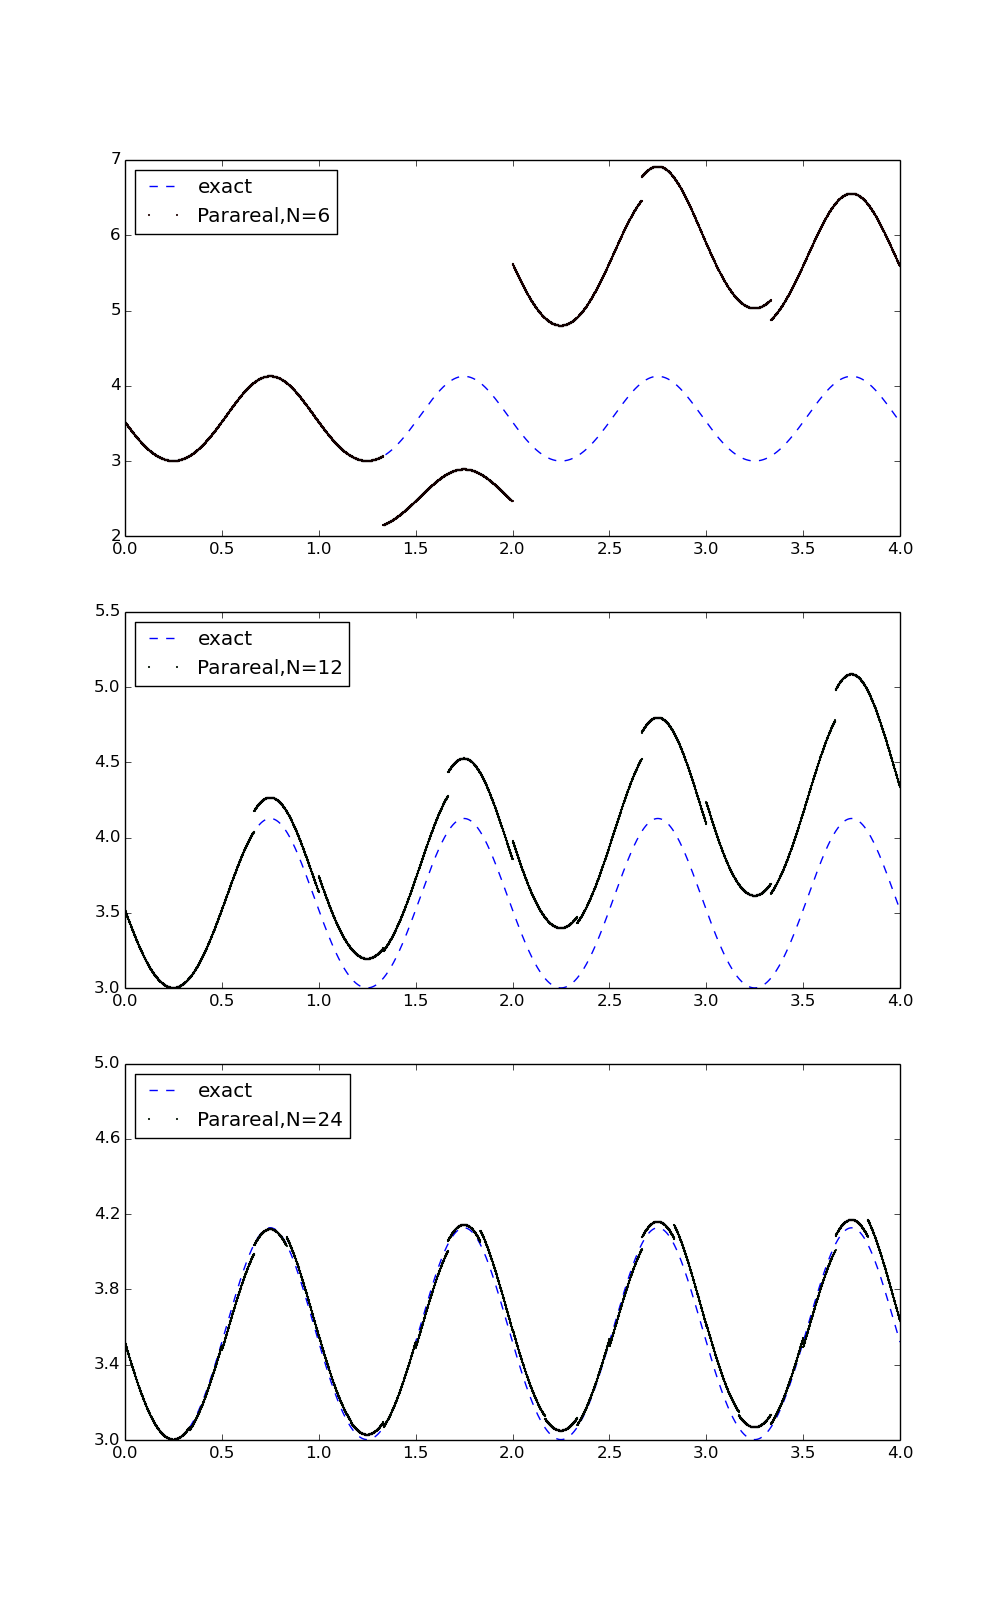
\includegraphics[scale=0.5]{parareal_img.png}
\caption{The result of 1 iteration of the Parareal algorithm on equation (\ref{Parareal_ODE_exs}), for three different time decompositions, $N=6,12,24$. }
\label{P_fig_1_itr}
\end{figure}
\chapter{Parareal-Based BFGS Preconditioner} \label{method_chap}
In the previous chapter we saw that the Parareal scheme allows us to parallelize time-dependent differential equations in their temporal direction. In this chapter we will present an approach on how to parallelize optimal control problems with time-dependent differential equation constraints in the temporal direction. 
\\
\\
This chapter consists of four sections. In the first section we decompose the time domain as we did in section \ref{Para_dcomp_sec}, only now in the context of control problems with time-dependent DE constraints. Decomposing the time interval leads to a reformulation of the control problem that includes extra constraints on the state equation. How to handle these new constraints are dealt with in section \ref{penalty_sec}. To solve this constrained problem, we use the same approach as \cite{maday2002parareal} namely the penalty method. The penalty approach is a simplified version of the augmented Lagrangian approach used in \cite{rao2016time} for parallel in time 4d variational data assimilation. We demonstrate the use of the penalty method by revisiting the example problem from section \ref{example_sec}.
\\
\\
In the third section a Parareal based preconditioner to be used in the optimization algorithms solving the optimal control problems is presented. This preconditioner originally proposed in \cite{maday2002parareal} is derived using ideas from subsection \ref{algebraic_sec} and we will in chapter \ref{Experiments chapter} see that it is crucial for the parallel in time algorithm to obtain any meaningful speedup. In the fourth and last section we propose a parallel in time method based on the penalty framework of section \ref{penalty_sec} and the BFGS optimization algorithm. The Parareal-based preconditioner from section \ref{pc sec} is used as an initial inverted Hessian approximation in the BFGS algorithm.
\section{Optimal Control Problem with Time-dependent DE Constraints on a Decomposed Time Interval} \label{decomp_sec}
We want to solve reducible optimization problems of type (\ref{OCP_DEF_J}-\ref{OCP_DEF_E}), where the state equation constraint $E(y(t),v,y_0)=0$ is time-dependent and solved on the interval $I=[0,T]$, with initial condition $y_0$. To introduce parallelism to our optimal control problem, we need to decompose the time domain and the state equation as we did in chapter \ref{parareal_chap}. 
\begin{definition}[Decomposed state equation] \label{DecompEDef}
Let $0=T_0<T_1<\cdots<T_{N-1}<T_N=T$ and define the $i$-th decomposed subinterval to be $I_i=[T_{i-1},T_i]$. We then introduce $N-1$ intermediate initial conditions $\Lambda=(\lambda_1,...,\lambda_{N-1})$, and set $\lambda_0=y_0$. Using these intermediate initial conditions we are able to define $N$ decomposed state equations:
\begin{align}
E^i(y_i(t),v,\lambda_{i-1})= 0 \quad t\in I_i. \label{DecompState}
\end{align} 
Solving the state equation $E(y(t),v,\Lambda)=0$ on the entire time domain, then means solving the $N$ decomposed equations (\ref{DecompState}) for $y_i$, and setting the state $y(t)$ to be:
\begin{align}
 y(t)=\left\{
     \begin{array}{lr}
		y_1(t)\quad t\in [T_0,T_1] \\
		y_2(t)\quad t\in(T_1,T_2] \\
		\cdots \quad\quad\cdots\\
		y_N(t)\quad t\in(T_{N-1},T_N]
	\end{array}
   \right.	\label{GatherState}
\end{align}
\end{definition}
\noindent
Using the decomposed time interval, state and state equation of definition \ref{DecompEDef}, we can define the decomposed optimal control problem. Since we want to solve the decomposed state equations simultaneously, the intermediate initial conditions $\Lambda$ will be added to the optimization problem as additional control variables. Because these variables are artificially introduced by us, we refer to $\Lambda$ as the virtual control, while we call the original control $v$ the real control. We also want the state to be continuous, so we need to introduce new constraints on the problem that enforces the continuity of $y(t)$. These new constraints are written up along with the decomposed reformulation of the optimal control problem in definition \ref{DecompOCPDef}.
\begin{definition}[Decomposed optimal control problem] \label{DecompOCPDef}
Let $Y,V,Z$ be defined as in definition \ref{OCP_def}. The decomposed optimal control problem with time-dependent DE constraint is the following minimization problem:
\begin{align}
\underset{y\in Y,v\in V,\Lambda}{\text{min}} \ &J(y(t),v,\Lambda),  \label{decomposed problem1}\\
\textrm{subject to:} \ &E(y(t),v,\Lambda)=0, \quad t\in [0,T]. \label{decomposed problem}
\end{align}
To enforce the continuity of $y(t)$ between subintervals, we introduce extra constraints:
 \begin{align}
y_{i}(T_i)=y_{i+1}(T_i)=\lambda_i \quad \ i=1,..,N-1. \label{Extra constraints}
\end{align}
\end{definition}
\noindent
If all the decomposed state equations $E^i(y_i,v,\lambda_{i-1})=0$ are uniquely solvable for all control variables $v\in V$, we can reduce the decomposed optimization problem from definition \ref{DecompOCPDef}. We write up the reduced version of problem (\ref{decomposed problem1}-\ref{Extra constraints}) in the next definition.
\begin{definition}[Decomposed and reduced optimal control problem] \label{DecompRedOCPDef}
Consider problem (\ref{decomposed problem1}-\ref{Extra constraints}). We assume that this problem is reducible, and can therefore define $\hat J:V\rightarrow\mathbb{R}$ as:
\begin{align*}
\hat J(v,\Lambda) = J(y(v,\Lambda)(t),v,\Lambda)
\end{align*}
The decomposed and reduced optimal control problem with time-dependent differential equation constraints is then the following constrained minimization problem:
\begin{align}
&\underset{v\in V,\Lambda}{\text{min}} \ \hat J(v,\Lambda), \label{constrained reduced j}\\
&y_{i}(T_i)=\lambda_i, \ \quad  i=1,...,N-1. \label{constrained reduced}
\end{align}
\end{definition}
\noindent
Unlike the undecomposed case, the reduced and decomposed optimal control problem is not unconstrained. A strategy for handling the extra constraints (\ref{constrained reduced}) is discussed in the next subsection.
\section{The penalty method} \label{penalty_sec}
To solve the constrained problem (\ref{constrained reduced j}-\ref{constrained reduced}), we will use the penalty method\cite{nocedal2006numerical}, which transforms constrained problems into a series of unconstrained problems. This is done by moving the constraints into the objective function $J(v)$. For each constraint a term is added to $J$, which is positive for variables that does not satisfy the constraint, but zero if it does. The penalization of the constraints can be done in different ways, but we will restrict ourself to the quadratic penalty method, where the the terms penalizing the constraints are quadratic. 
\begin{definition}[Quadratic penalty method]\label{QuadPenMethDef}
Consider the constrained optimization problem:
\begin{align}
\min_x f(x)\quad\textrm{subject to: } c_i(x)=0,\quad i=1,...,N, \label{general_opti}
\end{align}
Given a penalty parameter $\mu>0$, the quadratic penalty method defines an altered functional $f_{\mu}:X\rightarrow\mathbb{R}$ related to the functional of problem (\ref{general_opti}).
\begin{align}
f_{\mu}(x) = f(x) +\frac{\mu }{2}\sum_{i=1}^Nc_i(x)^2 \label{general_opti_pen}
\end{align}
Minimizing $f_{\mu}$ is an unconstrained optimization problem. If we now instead consider our decomposed optimization problem (\ref{constrained reduced j}-\ref{constrained reduced}), we can write up its penalized objective function $\hat J_{\mu}$ as:
\begin{align}
\hat J_{\mu}(v,\Lambda) = \hat J(v) + \frac{\mu}{2}\sum_{i=1}^{N-1}(y_{i}(T_i)-\lambda_i)^2. \label{pen_obj_J}
\end{align}
\end{definition}
\noindent
The idea of the penalty method is that the minimizer of (\ref{general_opti_pen}) should approach a feasible minimizer of (\ref{general_opti}) when we increase the penalty parameter $\mu$. Since the penalized problem can be difficult to solve for large $\mu$ values, the usual approach for solving constrained problems with the penalty method, is to minimize the penalized objective function for an increasing sequence of penalty parameters $\mu$. We write up the general algorithmic framework of the penalty method applied to problem (\ref{constrained reduced j}-\ref{constrained reduced}) in algorithm \ref{PEN_ALG}. 
\\
\\
\begin{algorithm}[H] 
\KwData{Choose $\mu_0,\tau_0>0$, and some initial control $(v^0,\Lambda^0$)}
\For{$k=1,2,...$}{
Find $(v^k,\Lambda^k)$ s.t. $\parallel\nabla \hat J_{\mu_{k-1}}(v^k,\Lambda^k)\parallel<\tau_{k-1}$\;
\eIf{STOP CRITERION satisfied}{
$\bold{Stop}$ algorithm\;
}{
Choose new $\tau_k\in(0,\tau_{k-1})$ and $\mu_k\in(\mu_{k-1},\infty) $\;
}
}
\caption{Penalty method \label{PEN_ALG}}
\end{algorithm}
\noindent
\\
If we want to use the penalty method, we need to know if the framework presented in algorithm \ref{PEN_ALG} is consistent. The penalty method is consistent, if for any given minimizer $(v,\Lambda)$ of $\hat J$, the iterates $(v^k,\Lambda^k)$ produced by framework \ref{PEN_ALG} converges to $(v,\Lambda)$, meaning:
\begin{align*}
\lim_{k\rightarrow \infty} (v^k,\Lambda^k) =(v,\Lambda).
\end{align*}
From \cite{nocedal2006numerical} we get a result that deals with this:
\begin{theorem} \label{consistency theorem}
Assume that $\forall k$, $(v^k,\Lambda^k)$ is the exact global minimizer of $J_{\mu_k}$ in context of the framework in algorithm \ref{PEN_ALG}. Then each limit point of the sequence $\{(v^k,\Lambda^k)\}$ is a solution of the problem (\ref{constrained reduced j}-\ref{constrained reduced}).
\end{theorem}
\begin{proof}
\cite{nocedal2006numerical}
\end{proof}
\noindent
Theorem \ref{consistency theorem} tells us that the penalty method of algorithm \ref{PEN_ALG} is consistent, if we for all $k$ can find an exact global minimizer of $J_{\mu_k}$. In practice, finding an exact minimizer of the penalized objective function is not always achievable. Another theorem from \cite{nocedal2006numerical} indicates what to expect if we are unable to find a global minimizer of $J_{\mu_k}$ for all $k$'s.
\begin{theorem} \label{feasible theorem}
If the tolerance $\tau_k$ and the penalty parameter $\mu_k$ of the method in algorithm \ref{PEN_ALG} satisfy
\begin{align*}
\lim_{k\rightarrow\infty} \tau_k =0,\quad \textrm{and} \quad \lim_{k\rightarrow\infty} \mu_k = \infty.
\end{align*}
the limit point of the the sequence $\{(v^k,\Lambda^k)\}$ will be a feasible point. In context of problem (\ref{constrained reduced j}-\ref{constrained reduced}), this means that:
\begin{align*}
\forall i=1,...,N-1\quad\lim_{k\rightarrow\infty}(y_{i}^k(T_i)-\lambda_i^k)=0 
\end{align*}
\end{theorem}
\begin{proof}
\cite{nocedal2006numerical}
\end{proof}
\noindent
Theorem \ref{consistency theorem} provides the theoretical consistency of the method in algorithm \ref{PEN_ALG}, this consistency is based on the assumption that we are able to minimize the penalized objective function for ever increasing penalty parameters $\mu$. Theorem \ref{feasible theorem} shows that the quadratic penalty method at least will produce a feasible control solution. In section \ref{consistency_sec} we will try to verify the consistency of algorithm \ref{PEN_ALG} for the example problem, and we will see that theorem \ref{consistency theorem} and \ref{feasible theorem} are crucial for understanding the results we get. 
\\
\\
We will now look at the most important part of the framework in algorithm \ref{PEN_ALG}, namely the optimization of the penalized objective function $\hat J_{\mu}$. To be able to optimize $\hat J_{\mu}$, we need its gradient, and we will therefore in the next section derive the gradient of the general penalized objective function (\ref{pen_obj_J}) using the adjoint approach. We will also find an expression for $\hat J_{\mu}'(v,\Lambda)$ for the example problem (\ref{exs_J}-\ref{exs_E}). In section \ref{pc sec} we will present a Parareal-based preconditioner, that we will use to improve the optimization of $\hat J_{\mu}$.
\subsection{The Gradient of the Penalized Objective Function}
We have introduced the penalized objective function (\ref{pen_obj_J}), that depends on both the real and virtual control, and we now want to evaluate its gradient. We again take the adjoint approach as we did in section \ref{adjointGrad_sec}, and the expression for $\hat J_{\mu}'(v,\Lambda)$ belonging to the general optimization problem (\ref{decomposed problem1}-\ref{decomposed problem}) is given in proposition \ref{penalty_grad_prop}.
\begin{proposition}[Gradient of the penalized objective function] \label{penalty_grad_prop}
Let $\hat J_{\mu}$ be the penalized objective function (\ref{pen_obj_J}). With similar assumptions as in proposition \ref{redGrad_prop}, the gradient of $\hat J_{\mu}$ is as follows: 
\begin{align}
\hat J_{\mu}'(v,\Lambda)=-(E_v(y(t),v,\Lambda)^*+E_{\Lambda}(y(t),v,\Lambda)^*)p(t)+ (\frac{\partial}{\partial v}+\frac{\partial}{\partial\Lambda})J_{\mu}(y,v,\Lambda). \label{pen_abs_grad}
\end{align}
The decomposed adjoint $p(t)$ is defined on $I=[0,T]$ as:
\begin{align}
 p(t)=\left\{
     \begin{array}{lr}
		p_1(t)\quad t\in [T_0,T_1] \\
		p_2(t)\quad t\in(T_1,T_2] \\
		\cdots \quad\quad\cdots\\
		p_N(t)\quad t\in(T_{N-1},T_N]
	\end{array}
   \right.	\label{GatherAdjoint}
\end{align}
where the $p_i$s are the solutions of the decomposed adjoint equations:
\begin{align}
E_{y_i}^i(y_i(t),v,\Lambda)^{*}p_i(t)=\frac{\partial}{\partial y_i}J_{\mu}(y_i,v,\Lambda), \quad t\in [T_{i-1},T_i]. \label{penalty adjoint}
\end{align}
\end{proposition}
\begin{proof}
Same reasoning as in proposition \ref{redGrad_prop}.
\end{proof}
\noindent
Notice that the state equation $E(y(t),v,\Lambda)=0$ consists of several equations defined separately on each of the decomposed subintervals. The result is that the adjoint equation also consists of several equations defined on each interval. To see this clearly we will derive the adjoint and the gradient for the example problem (\ref{exs_J}-\ref{exs_E}).
\subsection{Deriving the Adjoint for the Example Problem}
Before we derive the adjoint equation of the decomposed example problem (\ref{exs_J}-\ref{exs_E}) we need to write up the decomposed state equation and the penalized objective function. We start by decomposing the interval $[0,T]$ into $N$ subintervals $\{[T_{i-1},T_{i}]\}_{i=1}^{N}$. We can then define the decomposed state equation on each interval:
\begin{align}
\left\{
     \begin{array}{lr}
       	\frac{\partial}{\partial t} y^i(t)=a y^i(t) + v(t) \quad t\in(T_{i-1},T_{i})\\
       	y^i(T_{i-1})=\lambda_{i-1}
     \end{array}
   \right. \label{decomp_E}
\end{align}
We get the reduced penalized objective function by adding the the penalty terms to the unpenalized objective function (\ref{exs_J}):
\begin{align}
\hat J_{\mu}(v,\Lambda) = \frac{1}{2}\int_0^Tv(t)^2dt + \frac{\alpha}{2}(y(T)-y^T)^2 + \frac{\mu}{2}\sum_{i=1}^{N-1}(y^{i-1}(T_i)-\lambda_i)^2 \label{penalty_func}
\end{align}
Having formulated the penalized objective function, we are no ready to write up its gradient. The gradient of (\ref{penalty_func}) is given in proposition \ref{penGrad_prop}, but since the gradient depends on the decomposed adjoint equations, we write up these first.
\begin{proposition} \label{pen_adjoint_prop}
The decomposed adjoint equation of problem (\ref{exs_J}-\ref{exs_E}) on interval $[T_{N-1},T_N]$ is:
\begin{align}
\left\{
     \begin{array}{lr}
	-\frac{\partial }{\partial t}p_N =a p_N  \\
	p_N(T_{N}) = \alpha( y_N(T_{N})-y_T)
	\end{array}
   \right. \label{end adjoint}
\end{align}
On $[T_{i-1},T_i]$ the decomposed adjoint equations are:
\begin{align}
\left\{
     \begin{array}{lr}
	-\frac{\partial }{\partial t}p_i =ap_i  \\
	p_i(T_{i}) = \mu(y_{i}(T_{i})-\lambda_{i} )
	\end{array}
   \right. \label{exs_adjoint}
\end{align}
\end{proposition} 
\begin{proof}
The decomposed adjoint equation on interval $I_i= [T_{i-1},T_{i}]$ is defined by the equation $E^i_{y_i}(y_i,v,\Lambda)^*p_i=\frac{\partial}{\partial y_i}J_{\mu}(y_i,v,\Lambda)$. This means that to derive it, we need expressions for $E^i_{y_i}(y_i,v,\Lambda)^*$ and $\frac{\partial}{\partial y_i}J_{\mu}(y_i,v,\Lambda)$. We will use the same approach as in the proof of proposition \ref{adjoint_eq_prop}, meaning that we will use the weak formulation of the decomposed state equations to derive the adjoint. If we let $(\cdot,\cdot)_i$ denote the $L^2$ inner product on $(T_{i-1},T_i)$, we can define a bilinear form $\mathcal{E}^i$ as:
\begin{align*}
\mathcal{E}^i[y_i,\phi]=(y_i,(-\frac{\partial}{\partial t}-a+\delta_{T_i})\phi)_i - (v+\delta_{T_{i-1}}\lambda_{i-1},\phi)_i
\end{align*}
The weak formulation of the $i$-th state equation then reads:
\begin{align*}
\textrm{Find $y_i$ s.t.}\quad \mathcal{E}^i[y_i,\phi]=0 \quad \forall \phi\in C^{\infty}((T_{i-1},T_i)).
\end{align*}
Arguing similarly as we did in the proof of proposition \ref{adjoint_eq_prop}, we find the linearised adjoint of $\mathcal{E}^i$ to be:
\begin{align*}
\mathcal{E}_{y_i}^i[\cdot,\psi]^* = (\cdot,(\frac{\partial}{\partial t}-a+\delta_{T_{i-1}})\psi)_i
\end{align*}
The weak formulation of the $i$-th adjoint equation is then: Find $p_i$ such that $\mathcal{E}_{y_i}^i[p_i,\psi]^*=(\frac{\partial}{\partial y_i}J_{\mu}(y_i,v,\Lambda),\psi)_i$, $\forall\psi \in C^{\infty}$. If we can find an expression for $\frac{\partial}{\partial y_i}J_{\mu}$, we will have the weak adjoint equation. It turns out that we are able to decompose the penalized objective function into $N$ functions $J_{\mu}^i$ defined as:
\begin{align*}
J_{\mu}^i(y_i,v,\Lambda)& = \int_{T_{i-1}}^{T_i} v(t)^2 dt + \frac{\mu }{2}(y_i(T_i)-\lambda_i)^2, \quad \textrm{for }i=1,...,N-1,\ \textrm{and}\\
J_{\mu}^N(y_N,v,\Lambda) &= \int_{T_{N-1}}^{T_N} v(t)^2 dt + \frac{\alpha }{2}(y_N(T_N)-y^T)^2.
\end{align*}
We notice that the the sum of these decomposed objective functions equals the penalized objective function (\ref{penalty_func}). What we also see is that $J_{\mu}^i$ only depends on the $i$-th state equation. This means that $\frac{\partial}{\partial y_i}J_{\mu}=\frac{\partial}{\partial y_i}J_{\mu}^i$.
\begin{align*}
\frac{\partial}{\partial y}J_{\mu}^i(y_i,v,\Lambda) &= \mu\delta_{T_i}(y_i(T_i)-\lambda_i),\quad i=1,..,N-1, and \\
\frac{\partial}{\partial y}J_{\mu}^N(y_N,v,\Lambda) &= \delta_{T_N}\alpha(y_N(T_N)-y^T)
\end{align*}
For $i=1,...,N-1$, the weak formulation of the decomposed adjoint equations will look like:
\begin{align*}
\textrm{Find $p_i$ s.t.}\quad (p_i,(\frac{\partial}{\partial t}-a+\delta_{T_{i-1}})\psi)_i =(\mu\delta_{T_i}(y_i(T_i)-\lambda_i),\psi)_i \quad \forall \psi\in C^{\infty}((T_{i-1},T_i)).
\end{align*}
For $i=N$ the adjoint equation is almost identical to the above expression, with exception of the $(\mu\delta_{T_i}(y_i(T_i)-\lambda_i),\psi)_i$ term, which instead is replaced by $(\delta_{T_N}\alpha(y_N(T_N)-y^T),\psi)_i$. Using partial integration we can reformulate the weak formulations of the decomposed adjoint equations into the strong formulations stated in proposition \ref{pen_adjoint_prop}.
\end{proof}
\noindent
With the adjont equations we can find the gradient.
\begin{proposition} \label{penGrad_prop}
The gradient of (\ref{penalty_func}), $\hat J_{\mu}'$, with respect to the control $(v,\Lambda)$ is:
\begin{align}
\hat J_{\mu}'(v,\Lambda) = (v+p,p_{2}(T_1) -p_{1}(T_1),..., p_{N}(T_{N-1}) -p_{N}(T_{N-1})) \label{penalty grad}
\end{align}
\end{proposition}
\begin{proof}
Proposition \ref{penalty_grad_prop} states the gradient of the penalized objective function for a general decomposed problem in (\ref{pen_abs_grad}). To derive an expression for the gradient of our example problem, we need to differntiate the decomposed state equations and the penalized objective function with respect to the real and virtual control. We will again use the weak formulation of the state equation given in the proof of proposition \ref{pen_adjoint_prop} to find the different terms. The weak formulation of the $i$-th state equation is based on the bilinear form $\mathcal{E}^i[v,\phi]=(y_i,(-\frac{\partial}{\partial t}-a+\delta_{T_i})\phi)_i - (v+\delta_{T_{i-1}}\lambda_{i-1},\phi)_i$. Differentiating $\mathcal{E}^i$ with respect to the real and virtual control yields:
\begin{align*}
\mathcal{E}_v^i[\cdot,\phi] &= -(\cdot,\phi)_i, \quad i=1,...,N,\\
\mathcal{E}_{\lambda_{i-1}}^i[\cdot,\phi] &= -(\cdot,\delta_{T_{i-1}}\phi)_i,\quad i=2,...,N.
\end{align*}
Notice that both of these forms are symmetric, and we therefore do not need to do more work to find their adjoints. The strong interpretation of $\mathcal{E}_v^i$ and $\mathcal{E}_{\lambda_{i-1}}^i$, is that $\mathcal{E}_v^i$ is multiplication by minus one, while $\mathcal{E}_{\lambda_{i-1}}^i$ is multiplication by minus one and evaluation at $t=T_{i-1}$. Next we want to differentiate the decomposed objective functions $J_{\mu}^i$ also defined in the proof of proposition \ref{pen_adjoint_prop}.
\begin{align*}
\frac{\partial}{\partial v} J_{\mu}^i(y,v,\Lambda) &= v,\quad i=1,...,N, \\
\frac{\partial}{\partial \lambda_i}J_{\mu}^i(y,v,\Lambda) &= - \mu (y_{i}(T_i)-\lambda_i),\quad i=1,...,N-1.
\end{align*}
The last step of the proof is to insert the above derived expressions into formula (\ref{pen_abs_grad}). We separate the gradient into two parts, where the first part is the gradient with respect to the real control, while the second part are the components that depends on the virtual control. We start by stating $\frac{\partial}{\partial v} \hat J_{\mu}$:
\begin{align*}
\frac{\partial}{\partial v} \hat J_{\mu}(v,\Lambda) &= -E_v^*p +  \sum_{i=1}^N\frac{\partial}{\partial v} J_{\mu}^i(y_i,v,\Lambda) \\
&=p+v
\end{align*}
We then find the component of the gradient related to $\lambda_i$. Only the $i+1$-th state equation and the $i$-th decomposed objective function depends on $\lambda_i$. This yields:
\begin{align*}
\frac{\partial}{\partial \lambda_i} \hat J_{\mu}(v,\Lambda) &= -E_{\lambda_i}^{i+1}(y_{i+1},v,\Lambda)^* p_{i+1} +  \frac{\partial}{\partial \lambda_i} J_{\mu}^i(y_i,v,\Lambda) \\
&= p_{i+1}(T_i)-\mu (y_{i}(T_i)-\lambda_i)\\
 &= p_{i+1}(T_i)-p_i(T_i)
\end{align*}
Here we made use of $E_{\lambda_i}^{i+1}(y_{i+1},v,\Lambda)^*=-1$ and $p_i(T_i)=\mu (y_{i}(T_i)-\lambda_i)$ from (\ref{exs_adjoint}). Combining $\frac{\partial}{\partial v} \hat J_{\mu}$ and $ \frac{\partial}{\partial \lambda_i}$ for $i=1,..,N-1$ gives us the gradient (\ref{penalty grad}).
\end{proof} 
\section{Parareal Preconditioner} \label{pc sec}
Parallelizing the solution process of optimal control problems with time-dependent differential equation constraints comes down to solving a series of penalized control problems. Since we have derived the gradient of these penalized problems for a specific example, we can now solve the control problem numerically using an optimization algorithm. We can for example use the steepest descent method (\ref{SD_itr}), which would create the following iteration for each penalized control problem:
\begin{align}
(v^{k+1},\Lambda^{k+1}) = (v^{k},\Lambda^{k}) -\rho_k\nabla\hat{J}_{\mu}(v^{k},\Lambda^{k}) \label{gradient_method}
\end{align}
Alternatively we could use a BFGS iteration (\ref{BFGS_itr}), which would result in the following update:
\begin{align}
(v^{k+1},\Lambda^{k+1}) = (v^{k},\Lambda^{k}) -\rho_kH^{k}\nabla\hat{J}_{\mu}(v^{k},\Lambda^{k}) \label{bfgs_method}
\end{align}
Where $H^k$ is the inverse Hessian approximation defined in (\ref{inv_H_apr}). To improve convergence of the unconstrained optimization solvers, we include the Parareal-based preconditioner, proposed in \cite{maday2002parareal}, in our optimization algorithms. Assuming that $v\in\mathbb{R}^{n_v}$, the preconditioner $Q$ will be on the form:
\begin{align}
Q = \left[ \begin{array}{cc}
	\mathbbold{1} & 0 \\
	0 & Q_{\Lambda} \\
	\end{array} \right]\in \mathbb{R}^{n_v+N\times n_v+N},\quad Q_{\Lambda}\in\mathbb{R}^{N-1\times N-1} \label{PC_form}
\end{align} 
We see that $Q$ only affects the $N-1$ last components of the gradient, which is the part connected with the virtual control $\Lambda$. The real control $v$ is therefore not directly affected by $Q$. For steepest descent, we apply $Q$, by modifying (\ref{gradient_method}) in the following way:
\begin{align}
(v^{k+1},\Lambda^{k+1}) = (v^{k},\Lambda^{k}) -\rho_kQ\nabla\hat{J}_{\mu}(v^{k},\Lambda^{k}) \label{gradient_method2}
\end{align}
For us to expect any improvement in convergence for the preconditioned steepest descent, $Q$ would have to resemble the Hessian of $\hat{J}_{\mu}$, at least for the virtual part of the control. We also need $Q$ to be cheaply computable. Applying $Q$ to the BFGS iteration, is done by setting the initial Hessian approximation $H^0=Q$. To be able to do this, we need $Q$ to be symmetric positive definite, since that is a requirement on $H^0$. 
\\
\\
We derive $Q$ by looking at a constructed optimal control problem that we call the virtual problem. The virtual problem is a control problem decomposed as detailed in section \ref{decomp_sec}, but its objective function $\bold J$ is set to be the penalty terms, which only depends on the virtual control $\Lambda$. We already stated this problem in section \ref{algebraic_sec}, and by utilizing the algebraic Parareal formulation, we will try to find a good candidate for $Q_{\Lambda}$.
\subsection{Virtual Problem} \label{vir_sec}
The Parareal-based preconditioner only affects the part of the gradient connected to the virtual control $\Lambda$. To motivate and derive $Q$, we therefore consider an optimal control problem where the real control $v$ is removed, and the objective function only depends on $\Lambda$. We have already presented this problem in section \ref{algebraic_sec}, but we restate it here for future reference. However, before we do this let us first properly define the fine and coarse propagators.
\begin{definition}[Fine and coarse propagator] \label{prop_def}
Let $f(y(t),t)=0$ be a time-dependent differential equation without a source term. Given $\Delta T=\frac{T}{N}$ and an initial condition $\omega$, let $y_f$ and $y_c$ be a fine and a coarse numerical solution of the initial value problem:
\begin{align}
 \left\{
     \begin{array}{lr}
		f(y(t),t)=0 \ \quad \textrm{for $t \in (0,\Delta T)$} \\
		y(0)=\omega
	\end{array}
	\right.	
\end{align}
We then define the fine propagator as $\bold F_{\Delta T}(\omega) = y_f(\Delta T)$ and the coarse propagator as $\bold G_{\Delta T}(\omega) = y_c(\Delta T)$. We also define the lower triangonal matrices $M,\bar M\in\mathbb{R}^{N-1\times N-1}$ as: 
\begin{align*}
M= \left[ \begin{array}{cccc}
   \mathbbold{1} & 0 & \cdots & 0 \\  
   -\bold{F}_{\Delta T} & \mathbbold{1} & 0 & \cdots \\ 
   0 &-\bold{F}_{\Delta T} & \mathbbold{1}  & \cdots \\
   0 &\cdots &-\bold{F}_{\Delta T} & \mathbbold{1}  \\
   \end{array}  \right],
\bar M= \left[ \begin{array}{cccc}
   \mathbbold{1} & 0 & \cdots & 0 \\  
   -\bold{G}_{\Delta T} & \mathbbold{1} & 0 & \cdots \\ 
   0 &-\bold{G}_{\Delta T} & \mathbbold{1}  & \cdots \\
   0 &\cdots &-\bold{G}_{\Delta T} & \mathbbold{1}   \\
   \end{array}  \right].
\end{align*}
\end{definition}
\noindent
We then use the fine propagator $\bold F_{\Delta T}(\omega)$ to define the virtual problem.
\begin{definition}[Virtual problem]
Given a fine propagator $\bold F_{\Delta T}$, that solves a time-dependent differential equation $f(y(t),t)=0$, an initial condition $\lambda_0=y_0$ and the control variable $\Lambda=(\lambda_1,...,\lambda_ {N-1})$, the virtual control problem is:
\begin{align}
&\min_{\Lambda}\bold{J}(\Lambda,y) = \frac{1}{2}\sum_{i=1}^{N-1} (y_{i-1}(T_{i})-\lambda_{i})^2, \label{virtual_func} \\
&\textrm{subject to } \ y_{i-1}(T_{i}) = \bold F_{\Delta T}(\lambda_{i-1})\quad \textrm{for} \ i=1,...,N-1 \label{virtual}
\end{align}
We also recognize function (\ref{virtual_func}) as a least squares function, which we can write on vector notation as:
 \begin{align}
\bold J(y,\Lambda) = \frac{1}{2} x(\Lambda)^Tx(\Lambda), \label{non_lin_LS}
\end{align}
where the vector function $x:\mathbb{R}^{N-1}\rightarrow \mathbb{R}^{N-1}$ is:
\begin{align}
x(\Lambda)= M\Lambda=\left( \begin{array}{c}  
   \lambda_1 - \bold F_{\Delta T}(\lambda_0) \\ 
   \lambda_2 - \bold F_{\Delta T}(\lambda_1) \\
   \cdots  \\
   \lambda_{N-1} -\bold F_{\Delta T}(\lambda_{N-1}) \\
   \end{array}  \right).
\end{align}
\end{definition}
\noindent
In chapter \ref{parareal_chap} we explained how the virtual problem could be solved by setting $\lambda_i= \bold F_{\Delta T}(\lambda_{i-1})$, which is the same as solving $\bold J(\Lambda,y)=0$. This equation can be written up on matrix form as:
\begin{align}
M \ \Lambda = H. \label{Parareal_equation}
\end{align}
The $H$ on the right hand side of the above equation is the propagator applied to the initial condition:
\begin{align*}
H = \left[ \begin{array}{c}
   \bold F_{\Delta T}( y_0) \\
   0 \\
   \cdots \\
   0 \\
   \end{array}  \right].
\end{align*}
In section \ref{algebraic_sec} we mentioned that the Parareal algorithm could be reformulated as a preconditioned fix point iteration solving equation (\ref{Parareal_equation}). This can be expressed in matrix form as follows:
\begin{align}
\Lambda^{k+1} = \Lambda^k + \bar{M}^{-1}(H-M\Lambda^k)\label{par_mat_sys}
\end{align}
Where $\bar{M}$ is the coarse version of the matrix $M$ stated in definition \ref{prop_def}. When we are solving the original optimal control problem we do not try to find a triple $(v,\Lambda,y)$ that solves $J_{\mu}(v,\Lambda,y)=0$. Instead we try to solve $\hat J_{\mu}'(v,\Lambda)=0$. To find the Parareal-based preconditioner, we therefore try to find a similar expression to (\ref{Parareal_equation}) for $\bold{\hat{J}}'(\Lambda)=0$. To be able to find this expression, we first need to define the coarse and fine adjoint propagators.
\begin{definition}[Fine and coarse adjoint propagator] \label{adjoint_prop_def}
Let $f(y(t),t)=0$ be a time-dependent differential equation. Given $\Delta T$, a state $y(t)$ and an initial condition $\omega$, let $p_f$ and $p_c$ be a fine and a coarse numerical solution of the initial value problem:
\begin{align}
 \left\{
     \begin{array}{lr}
		f'(y(t),t)^*p(t)=0 \ \quad \textrm{for $t \in (0,\Delta T)$} \\
		p(\Delta T)=\omega
	\end{array}
	\right.	
\end{align}
We then define the fine adjoint propagator as $\bold F_{\Delta T}^*(\omega) = p_f(0)$ and the coarse adjoint propagator as $\bold G_{\Delta T}^*(\omega) = p_c(0)$. We also define adjoint versions of the matrices $M$ and $\bar M$ as: 
\begin{align*}
M^*= \left[ \begin{array}{cccc}
   \mathbbold{1} & -\bold{F}_{\Delta T}^* & 0 & 0 \\  
   0 & \mathbbold{1} & -\bold{F}_{\Delta T}^* & \cdots \\ 
   \cdots &0 &  \mathbbold{1} & -\bold{F}_{\Delta T}^* \\
   0 &\cdots &\cdots &  \mathbbold{1}  \\
   \end{array}  \right],
\bar M^*= \left[ \begin{array}{cccc}
   \mathbbold{1} & -\bold{G}_{\Delta T}^* & 0 & 0 \\  
   0 & \mathbbold{1} & -\bold{G}_{\Delta T}^* & \cdots \\ 
   \cdots &0 &  \mathbbold{1} & -\bold{G}_{\Delta T}^* \\
   0 &\cdots &\cdots &  \mathbbold{1}  \\
   \end{array}  \right].
\end{align*}
\end{definition} 
\noindent
Using the matrices from definition \ref{adjoint_prop_def} we can write up the following proposition concerning the gradient of the reduced objective function of the virtual problem.
\begin{proposition} \label{vir_grad_prop}
The reduced objective function of the virtual problem (\ref{virtual_func}-\ref{virtual}) is:
\begin{align}
\bold{\hat J}(\Lambda) = \frac{1}{2}\sum_{i=1}^{N-1} (\bold F_{\Delta T}(\lambda_{i-1})-\lambda_{i})^2.\label{reduced_viritual}
\end{align}
Solving $\bold{\hat J}'(\Lambda)=0$ is equivalent to resolving the system:
\begin{align}
M^* \ M \ \Lambda \ = \ M^* \ H. \label{vir_grad_sys}
\end{align}
A preconditioned fix point iteration for equation (\ref{vir_grad_sys}) inspired by the Parareal formulation (\ref{par_mat_sys}) is therefore:
\begin{align}
\Lambda^{k+1} = \Lambda^k + \bar{M}^{-1}\bar M^{-*}(M^*H-M^*M\Lambda^k). \label{grad_fix_iter}
\end{align}
\end{proposition}
\begin{proof}
We have already derived the gradient of $\bold{\hat J}$ in (\ref{penalty grad}). There we stated the gradient for the penalized version of the example problem (\ref{exs_J}-\ref{exs_E}). If we ignore the part of this gradient related to the real control $v$, we get the following expression for $\bold{\hat J}'$:
\begin{align*}
\hat{\bold J}'(\Lambda) = \{p_{i+1}(T_i)-p_{i}(T_i)\}_{i=1}^{N-1}.
\end{align*}
Here $p_i$ refers to the decomposed adjoint equation on interval $[T_{i-1},T_{i}]$. We now want to show that setting $p_{i+1}(T_i)-p_{i}(T_i)=0$ for $i=1,...,N-1$ is equivalent to equation \ref{vir_grad_sys}. To do this we will simply write out the expression $M^*(M\Lambda-H)$ and show that it equals $\hat{\bold J}'(\Lambda)$. We start with $M\Lambda-H$.
\begin{align*}
M \ \Lambda - H  = \left( \begin{array}{c}
	\lambda_1-\bold{F}_{\Delta T}(\lambda_0)\\
	\lambda_2-\bold{F}_{\Delta T}(\lambda_1) \\
	\cdots \\
	\lambda_{N-1}-\bold{F}_{\Delta T}(\lambda_{N-1}) 
	\end{array} \right).
\end{align*}
Notice that $\bold{F}_{\Delta T}(\lambda_{i-1})-\lambda_i$ is the initial condition of $i$-th adjoint equation, i.e. $p_i(T_i)=\bold{F}_{\Delta T}(\lambda_{i-1})-\lambda_i$. By exploiting this, and multiplying $M\Lambda-H$ with $M^*$ we get:
\begin{align}
M^* (M \ \Lambda-H)&=
	\left( \begin{array}{c}
	 \bold{F}_{\Delta T}^*(p_2( T_2))-p_1(T_1)\\
	\bold{F}_{\Delta T}^*(p_3( T_3))-p_2(T_2)\\
	\cdots \\
	-p_{N-1}(T_{N-1})
	\end{array} \right)
	\\
	&=\left( \begin{array}{c}
	p_2(T_1)-p_1(T_1)\\
	p_3(T_2)-p_2(T_2)\\
	\cdots \\
	p_{N-1}(T_{N-2})-p_{N-2}(T_{N-2}) \\
	-p_{N-1}(T_{N-1})
	\end{array} \right).
\end{align}
The last step is done by using $p_i(T_{i-1})=-F_{\Delta T}^*(-p_i(T_i))$, and this is possible since the adjoint equation is linear. We see that the $i$-th component of $M^* (M \Lambda-H)$ is equal to $p_{i+1}(T_i)-p_{i}(T_i)$ for $i\neq N-1$. The last component of $M^* (M \Lambda-H)$ is $-p_{N-1}(T_{N-1})$, and we are therefore missing $p_N(T_{N-1})$. This is however unproblematic since in context of the the virtual problem $p_N(T_{N-1})=0$. This shows us that $\hat{\bold J}'(\Lambda)= M^* (M \Lambda-H)$, which means that $\hat{\bold J}'(\Lambda)=0 \iff M^*M\Lambda =M^*H$. Since $\bar M$ and $\bar M^*$ approximates $M$ and $M^*$, $\bar{M}^{-1}\bar M^{-*}$ would be a natural preconditioner for a fix point iteration solving $M^*M\Lambda =M^*H$. 
\end{proof}
\noindent
Proposition \ref{vir_grad_prop} motivates $Q_{\Lambda}=\bar{M}^{-1}\bar M^{-*}$ as a preconditioner for solvers of decomposed and penalized optimal control problems, and this is actually the Parareal-based preconditioner proposed in \cite{maday2002parareal}. Inserting $Q_{\Lambda}$ into $Q$ yields the following:
\begin{align}
Q = \left[ \begin{array}{cc}
	\mathbbold{1} & 0 \\
	0 &  \bar{M}^{-1}\bar{M}^{-*}\\
	\end{array} \right]. \label{Q_PC}
\end{align}  
In \cite{maday2002parareal} $Q$ is proposed as a preconditioner for a steepest descent method. Other than to motivate $Q$ the authors of \cite{maday2002parareal} do not explore or derive any properties of the Parareal-based preconditioner. We are however interested in using $Q$ in combination with the BFGS algorithm, and to be able to do this we need to know that $Q$ is positive definite and that it is related to the Hessian of the objective function. We are also interested in the computational cost of $Q$. We will investigate the properties of the preconditioner by looking at the least squares formulation (\ref{non_lin_LS}) of problem (\ref{reduced_viritual}).
\subsection{Properties of the Parareal-Based Preconditioner}
We want to investigate the properties of $Q_{\Lambda}=\bar{M}^{-1}\bar{M}^{-*}$, and to do this we will show that $\bar{M}^{1}\bar{M}^{*}$ is an approximation to the Hessian of $\hat{\bold J}(\Lambda)$. To calculate the Hessian we use the least squares formulation (\ref{non_lin_LS}) of the virtual objective function. 
\begin{proposition}[Virtual Hessian]\label{NonLin_prop}
The Hessian of function (\ref{non_lin_LS}) is
\begin{align*}
\nabla^2 \hat{\bold J}(\Lambda) &= \nabla x^T\nabla x + \sum_{i=1}^{N-1} \nabla^2 x_i(\Lambda) x_i(\Lambda)\\
&=M(\Lambda)^TM(\Lambda) + D(\Lambda)
\end{align*}
Here $D(\Lambda)$ is a diagonal matrix with diagonal entries 
\begin{align*}
D_i=-\bold{F}_{\Delta T}''(\lambda_i)(\lambda_{i+1}-\bold F_{\Delta T}(\lambda_i)) \quad i=1,...,N-1,
\end{align*}
while $M(\Lambda)$ is the linearised forward model:
\begin{align*}
M(\Lambda) &= \left[ \begin{array}{cccc}
   \mathbbold{1} & 0 & \cdots & 0 \\  
   -\bold{F}_{\Delta T}'(\lambda_{1}) & \mathbbold{1} & 0 & \cdots \\ 
   0 &-\bold{F}_{\Delta T}'(\lambda_{2}) & \mathbbold{1}  & \cdots \\
   0 &\cdots &-\bold{F}_{\Delta T}'(\lambda_{N-1}) & \mathbbold{1}  \\
   \end{array}  \right]
\end{align*}	
\end{proposition}
\begin{proof}
We start by differentiating $\hat{\bold J}$:
\begin{align*}
\nabla \hat{\bold J}(\Lambda) &=  \nabla x(\Lambda)^T x(\Lambda)\\
&=\sum_{i=1}^{N-1} \nabla x_i(\Lambda) x_i(\Lambda)
\end{align*}
If we now differentiate $\nabla \hat{\bold J}$, we get:
\begin{align*}
\nabla^2 \hat{\bold J}(\Lambda) &= \nabla x^T\nabla x + \sum_{i=1}^{N-1} \nabla^2 x_i(\Lambda) x_i(\Lambda)
\end{align*}
We see that $\nabla x(\Lambda)=M(\Lambda)$, by looking at $\frac{\partial x_i}{\partial \lambda_j}$
\begin{align*}
\frac{\partial x_i}{\partial \lambda_j} = \left\{
     \begin{array}{lr}
		1 \quad\quad\quad\quad\quad i=j\\
		-\bold F_{\Delta T}'(\lambda_{j}) \quad i>1 \wedge j=i-1 \\
		0 \quad\quad\quad\quad\quad i\neq j \vee j\neq i-1
	\end{array}
   \right.	
\end{align*}
We can similarly find $\nabla^2 x_i$ by differentiating $x$ twice:
\begin{align*}
\frac{\partial^2 x_i}{\partial \lambda_j\partial\lambda_k} = \left\{
     \begin{array}{lr}
		-\bold F_{\Delta T}''(\lambda_{j}) \quad i>1 \wedge j=k=i-1 \\
		0 \quad\textrm{in all other cases}
	\end{array}
   \right.	
\end{align*}
Summing up the terms $\nabla^2 x_i(\Lambda)x_i(\Lambda)$ yields the diagonal matrix $D(\Lambda)$.
\end{proof}
\noindent
The first term of $\nabla^2 \hat{\bold J}(\Lambda)=M(\Lambda)^TM(\Lambda) + D(\Lambda)$ resembles $M^*M$ from the previous section, while the second term $D(\Lambda)$ is new. $D(\Lambda)$ is a diagonal matrix where the diagonal entries consists of products between the second derivative of $\bold F_ {\Delta T}$ and the residuals $\lambda_{i+1}-\bold F_{\Delta T}(\lambda_i)$. If the governing equation of the propagator $\bold F_ {\Delta T}$ is linear, $\bold F_{\Delta T}''(\lambda_i)=0$. This would again mean that $D(\Lambda)=0$ and that $\nabla^2 \hat{\bold J}(\Lambda)=M(\Lambda)^TM(\Lambda)$. We will therefore split our discussion of the Hessian of $\hat{\bold J}$ into two cases. In the first we assume the state equation is linear, while in the second case we discuss problems with non-linear state equations.
\subsubsection{Linear State Equations}
Assuming that the state equation is linear means that $\nabla^2 \hat{\bold J}(\Lambda)=M(\Lambda)^TM(\Lambda)$. Differentiating the propagator $\bold F_{\Delta T}$ is the same as linearising its governing equation. When the governing equation is itself linear, linearising it does not change the equation. Therefore $\bold F_{\Delta T}'(\lambda_i)\lambda_i = \bold F_{\Delta T}(\lambda_i)$. This means that the $M$ matrix from section \ref{vir_sec} is equal to $M(\Lambda)$. The same is true for $M^*$ and $M(\Lambda)^T$. Since  $\nabla^2 \hat{\bold J}(\Lambda)=M^*M$ we see that the Parareal-based preconditioner proposed in \cite{maday2002parareal} is in fact related to the inverse Hessian of the reduced penalized objective function. Furthermore if we can show that $\bar M^*\bar M$ is a positive definite matrix, we can use $Q$ as an initial approximation of the inverse Hessian in the BFGS optimization algorithm. This is as we will see in the following proposition indeed the case.
\begin{proposition} \label{pos_def_prop}
If $\bold G_{\Delta T}$ and $\bold G_{\Delta T}^*$ are based on consistent numerical methods, that is $\bar M^*=\bar M^T$, then the matrix $\bar M^*\bar M$ is positive definite.
\end{proposition}
\begin{proof}
If $\bold G_{\Delta T}$ and $\bold G_{\Delta T}^*$ are based on consistent numerical methods, that is if $\bold G_{\Delta T}(\omega)=\bold G_{\Delta T}^*(\omega)$. When inserting this into the matrices $\bar M$ and $\bar M^*$ from definition \ref{prop_def} and \ref{adjoint_prop_def}, we clearly see that $\bar M^*=\bar M^T$. For $M^*M$ to be positive definite, the following two conditions must hold:
\begin{align*}
&1.\quad x^T\bar M^*\bar Mx \geq 0 \quad \forall x\in\mathbb{R}^{N-1} \\
&2.\quad x^T\bar M^*\bar Mx =0 \iff x=0
\end{align*}
The first conditions hold due to $\bar M^*=\bar M^T$:
\begin{align*}
x^T\bar M^*\bar Mx = (\bar Mx)^T\bar Mx = ||Mx||^2 \geq 0.
\end{align*}
The second condition hold if $\bar M$ is invertible. This is true because $\bar M$ is a triangular matrix, with identity on its diagonal, and therefore has a determinant equal to 1. The determinant of a matrix being unequal to zero is equivalent with it being invertible, which means that $\bar M$ is invertible. This also means that $M^*M$ is positive definite, since both requirements for positive definiteness are satisfied. 
\end{proof}
\noindent
Proposition \ref{pos_def_prop} shows that the $\bar M^*\bar M$ matrix stemming from the virtual problem is positive definite. We can therefore use it as an initial Hessian approximation in the BFGS algorithm, at least as long as $\bold G_ {\Delta T}$ and $\bold G_ {\Delta T}^*$ are consistent. Now let us take a look at the case where the governing equation of $\bold F_{\Delta T}$ is non-linear.
\subsubsection{Non-Linear State Equations}
Unlike the Hessian of the linear problem the Hessian of the non-linear problem consists of two parts. One is the linearised forward model multiplied with its adjoint, while the second part is a diagonal matrix related to the second derivative of the propagator $\bold F_{\Delta T}$, and the residuals $\lambda_i-\bold F_{\Delta T}$. The first part of $\nabla^2 \bold{\hat{J}}$ is analogue to the Hessian of the linear problem. It is symmetric positive definite, and taking its inverse corresponds to first applying the backwards model, and then the forward model. What makes the Hessian of the non-linear problematic is therefore its second term. The first issue with the diagonal matrix $D(\Lambda)$, is how to calculate $\bold F_{\Delta T}''$. Another issue is that we can not guarantee that the sum of $M(\Lambda)^TM(\Lambda)$ and $D(\Lambda)$ is a positive matrix, and the same problem would arise in a coarse approximation of $\nabla^2 \bold{\hat{J}}$. The lack of positivity is a problem since we want to use the coarse approximation as an initial inverted Hessian approximation in the BFGS-algorithm.
\\
\\
One way to get around the $D(\Lambda)$ term in the Hessian for non-linearly constrained problem, is simply to ignore it. This leaves us with the $M(\Lambda)^TM(\Lambda)$ term, which we know how to deal with. Ignoring the term depending on the second derivative and the residual is actually a known strategy, called the Gauss-Newton method, for solving non-linear least square problems. Details on this method can be found in \cite{nocedal2006numerical}. A justification for this approach, is that at least in instances where we are close to a solution, the $\lambda_i-\bold F_{\Delta T}$ terms will be close to zero, and the $M(\Lambda)^TM(\Lambda)$ term will therefore dominate the Hessian. Ignoring the $D(\Lambda)$ term means that we can define an inverse Hessian approximation based on a coarse propagator $\bold G_{\Delta T}$ in the same way as we did for the problem with linear state equation constraints. This means that we define a matrix $\bar M(\Lambda)$:
\begin{align}
\bar M(\Lambda) &= \left[ \begin{array}{cccc}
   \mathbbold{1} & 0 & \cdots & 0 \\  
   -\bold{G}_{\Delta T}'(\lambda_{1}) & \mathbbold{1} & 0 & \cdots \\ 
   0 &-\bold{G}_{\Delta T}'(\lambda_{2}) & \mathbbold{1}  & \cdots \\
   0 &\cdots &-\bold{G}_{\Delta T}'(\lambda_{N-1}) & \mathbbold{1}  \\
   \end{array}  \right] \label{ppc_linearized}
\end{align}
The term $\bar{M}(\Lambda)^{-1}\bar{M}(\Lambda)^{-*}$ can then be used in an approximation of the inverse Hessian, as detailed in section \ref{vir_sec}.
\subsection{Parareal-based Precoditioner for the Example Problem}
To illustrate what $Q$ actually will look like we write up $\bar M^*\bar M$ for our example problem (\ref{exs_J}-\ref{exs_E}). The state and adjoint equation of this problem is:
\begin{align}
y'(t) &= ay(t) + v(t), \label{ppc_state} \\
p'(t) &= -ap(t). \label{ppc_adjoint}
\end{align}
The state equation includes a source term, which will not be included in the governing equation of the propagators, since the propagators are based on the virtual sourceless problem. This means that the governing equation of $\bold G_{\Delta T}$ is $y'(t) = ay(t)$. Alternatively we could let (\ref{ppc_state}) govern $\bold G_{\Delta T}$, but instead use $\bar M(\Lambda)$ from (\ref{ppc_linearized}) in our preconditioner, which would produce the same result. 
\\
\\
Let us now try to write out $\bar M^*\bar M$ for our example problem, when we have decomposed the time interval into $N$ subintervals. We first need to choose a numerical method to discretize the state and adjoint. In this example we will use the implicit Euler scheme from section \ref{FD_sub_sec}, with $\Delta T=\frac{T}{N}$. We can then write up $\bold G_{\Delta T}(\omega)$ and $\bold G_{\Delta T}^*(\omega)$:
\begin{align}
\frac{\bold G_{\Delta T}(\omega)-\omega}{\Delta T}&=  a\bold G_{\Delta T}(\omega) \\
&\Rightarrow \bold G_{\Delta T}(\omega)= \frac{\omega}{1-a\Delta T} \\
\frac{\omega-\bold G_{\Delta T}^*(\omega)}{\Delta T}&= -a\Delta T \bold G_{\Delta T}^*(\omega) \\
&\Rightarrow \bold G_{\Delta T}^*(\omega)= \frac{\omega}{1-a\Delta T} \label{ImplicitEG}
\end{align}
Since $\bold G_{\Delta T}(\omega)= \bold G_{\Delta T}^*(\omega)$, using implicit Euler both forwards and backwards produce consistent coarse propagators. We can now write up an exact expression for $\bar M\in\mathbb{R}^{N-1\times N-1}$. 
\begin{align*}
\bar M = \left[ \begin{array}{cccc}
   	1 & 0 & \cdots & 0 \\  
   	-\frac{1}{1-a\Delta T} & 1 & 0 & \cdots \\ 
   	0 &-\frac{1}{1-a\Delta T} & 1  & \cdots \\
   	0 &\cdots &-\frac{1}{1-a\Delta T} & 1  \\
  	\end{array}  \right].
\end{align*}
By traversing $\bar M$ we get $\bar M^*$. When we apply $Q$, we are not using $\bar M^*\bar M$, but instead its inverse. Let us illustrate how to apply the inverse of $\bar M^*\bar M$ to the virtual gradient through an example, wehere we set $N=4$. We first decompose $I=[0,T]$ into four sub-intervals $[T_0,T_1], [T_1,T_2], [T_2,T_3]$ and $[T_3,T_4]$. If we then evaluate the discrete gradient for a real control variable $v\in\mathbb{R}^{n+1}$ and a virtual control $\Lambda =(\lambda_1,\lambda_2,\lambda_3)$, the result is $\hat J_{\mu}(v,\Lambda)\in\mathbb{R}^{N+n}$. Multiplying $Q$ with $\hat J_{\mu}(v,\Lambda)$ will only affect its three last components, which we name $J_{\lambda_1},J_{\lambda_2}$ and $J_{\lambda_3}$. Applying $Q$ to $\hat J_{\mu}$ is done in two steps. We first multiply with $\bar M^{-*}$ based on on the propagator $\bold G_{\Delta T}^*= -\frac{1}{1-a\Delta T} $ 
\begin{align*}
\bar{J_{\lambda_1}} &=J_{\lambda_1} -\frac{1}{1-a\Delta T}(J_{\lambda_2} -\frac{1}{1-a\Delta T}J_{\lambda_3})\\
\bar{J_{\lambda_2}} &=J_{\lambda_2} -\frac{1}{1-a\Delta T}J_{\lambda_3}\\
\bar{J_{\lambda_3}} &=J_{\lambda_3} 
\end{align*} 
The second step is then to apply the forward system based on the coarse propagator $\bold G_{\Delta T}= -\frac{1}{1-a\Delta T} $:
\begin{align*}
\bar{\bar{J_{\lambda_1}}}&=\bar{J_{\lambda_1}} \\
\bar{\bar{J_{\lambda_2}}}&=\bar{J_{\lambda_2}}-\frac{1}{1-a\Delta T}\bar{J_{\lambda_1}} \\
\bar{\bar{J_{\lambda_3}}}&=\bar{J_{\lambda_3}} -\frac{1}{1-a\Delta T}(\bar{J_{\lambda_2}}-\frac{1}{1-a\Delta T}\bar{J_{\lambda_1}})
\end{align*} 
The result of multiplying $Q$ with the discrete penalized gradient is that the three last components of $\hat J_{\mu}(v,\Lambda)$ is changed to $\bar{\bar{J_{\lambda_1}}},\bar{\bar{J_{\lambda_2}}}$ and $\bar{\bar{J_{\lambda_3}}}$. 
\\
\\
an important special case of the Parareal-based preconditioner is the case when $N=2$. If we decompose the time domain into $N=2$ subdomains, both $\bar M$ and $\bar M^*$ becomes the identity matrix. This means that for $N=2$, $Q=\mathbbold{1}$, and therefore $Q$ has no effect. Since the preconditioner has no effect for $N=2$, we might also expect that for "small" $N$ the impact of applying $Q$ to the penalized gradient is only modest, and that the usefulness of $Q$ only materializes for higher values of decomposed subintervals $N$.
\subsubsection{Computational Cost of Parareal-Based Preconditioner}
The last aspect of the preconditioner $Q$ (\ref{Q_PC}), that we have yet not discussed is its computational cost. For $Q$ to be an effective preconditioner it needs to be cheap to compute. As the above example for $N=4$ shows, applying $Q_{\Lambda}$ to the virtual part of the gradient $\hat J_{\mu}'(v,\Lambda)$, comes down to first solving the linearised backward model, and then the linearised forward model on mesh of size $N$. This will translate to a computational cost of $\mathcal{O}(N)$. Here we have of course assumed that the state and adjoint equations are ODEs, and that the coarse propagator $\bold G_{\Delta T}$ is based on a finite difference scheme as in (\ref{ImplicitEG}). If we we instead were solving a PDE, the cost of applying $Q$ would also include computations done in spacial direction. If the spacial discretization has size $\mathcal{M}$, the cost of $Q$ would instead be $\mathcal{O}(\mathcal{M}N)$, but this could again be made cheaper by using a coarse resolution in space for $\bold G_{\Delta T}$. 
\\
\\
For $\mathcal{O}(N)$ to be considered a cheap operation, we require $N<<n$, where $n$ is the number of fine time steps. Since $N$ is the number of decomposed subintervals, $N$ does also equal the maximal number of processes that can be used to parallelize in time. If we want to increase the number of processes, we also need to increase $N$. This creates an upper limit for the scalability of our algorithm, when we use the Parareal-based preconditioner. For a fixed problem size $n$, the absolute upper limit of processes that can be used is $N=n$, but since we need a cheap to compute $Q$, this limit is in practice lower.  
\section{Summary and Presentation of Algorithm} \label{Algorithm_sec}
In the previous section we presented and derived properties of the Parareal-based preconditioner $Q$ introduced in \cite{maday2002parareal}. We showed that $Q$ is symmetric positive definite, and that it approximates the inverse Hessian of $\hat J_{\mu}$, at least for the part connected to the virtual control. We can therefore use $Q$ as an initial inverted Hessian approximation in the BFGS or L-BFGS optimization algorithms for minimization of the penalized objective function $\hat J_{\mu}(v,\Lambda)$ (\ref{constrained reduced j}). Combining the preconditioned BFGS solver with the quadratic penalty method of algorithm \ref{PEN_ALG} makes us able to propose algorithm \ref{PPC_PEN_ALG} as a parallel in time method for solving optimization problems with time-dependent DE constraints.
\\
\\
\begin{algorithm}[H] 
\KwData{Choose $\mu_0,\tau_0>0$, and some initial control $(v^0,\Lambda^0$)}
\For{$k=1,2,...$}{
$(v_0^k,\Lambda_0^k) \leftarrow (v^{k-1},\Lambda^{k-1})$\;
$H^0 \leftarrow Q(\Lambda_0^{k})$\;
$j\leftarrow0$\;
\While{$||\hat J'_{\mu_{k-1}}(v_j^k,\Lambda_j^k)||\geq \tau_{k-1}$ }{
$(v_{j+1}^k,\Lambda_{j+1}^k) \leftarrow (v_j^k,\Lambda_j^k) - \rho^j H^j \hat J'_{\mu_{k-1}}(v_j^k,\Lambda_j^k) $\tcp*[h]{In parallel}\;
Update $H^{j+1}$\;
$H^0 \leftarrow Q(\Lambda_{j+1}^k)$\;
$j\leftarrow j+1$\;
}
$(v^{k},\Lambda^{k})\leftarrow(v_{j}^k,\Lambda_{j}^k)$\;
\eIf{STOP CRITERION on $(v^{k},\Lambda^{k})$ satisfied}{
$\bold{Stop}$ algorithm\;
}{
Choose new $\tau_k\in(0,\tau_{k-1})$ and $\mu_k\in(\mu_{k-1},\infty) $\;
}
}
\caption{Quadratic penalty method with preconditioned BFGS optimization\label{PPC_PEN_ALG}}
\end{algorithm}
\noindent
\\
What separates algorithm \ref{PPC_PEN_ALG} from the general quadratic penalty method in algorithm \ref{PEN_ALG} is that the optimization step is done using BFGS (or L-BFGS) with $H^0=Q$. The most computationally costly part of algorithm \ref{PPC_PEN_ALG}, is the optimization step of the BFGS algorithm:
\begin{align}
(v_{j+1},\Lambda_{j+1}) = (v_j,\Lambda_j) - \rho^j H^j \hat J'_{\mu}(v_j,\Lambda_j) \label{BFGSupdate}
\end{align}
In section \ref{optiSec} we explained how general line search methods are applied, and also how one updates the inverse Hessian approximation in the BFGS and L-BFGS algorithms. Let us however briefly discuss how the update (\ref{BFGSupdate}) is done in context of the  minimization of our decomposed and penalized objective function (\ref{general_opti_pen}). Executing update (\ref{BFGSupdate}) is done in four steps:
\begin{align*}
1.\quad&\textit{Evaluate $\hat J'_{\mu}(v_j,\Lambda_j)$.} \\
2.\quad&\textit{Apply $H^j$ to $\hat J'_{\mu}(v_j,\Lambda_j)$.}\\
3.\quad&\textit{Find step length $\rho^j$} \\
4.\quad&\textit{Set $(v_{j+1},\Lambda_{j+1}) = (v_j,\Lambda_j) - \rho^j H^j \hat J'_{\mu}(v_j,\Lambda_j)$} 
\end{align*}
The first step of the above procedure, is to evaluate the gradient of $\hat J_{\mu}$. We know from proposition \ref{penalty_grad_prop}, that this requires us to first solve the decomposed state equations, and then the decomposed adjoint equations. We can solve the decomposed state equations and then the decomposed adjoint equations in parallel, since they are defined independently of each other on the decomposed subintervals. Applying $H^j$ to $\hat J'_{\mu}(v_j,\Lambda_j)$ is done using the recursive formula defining the $H^j$ update:
\begin{align}
H^j \hat J_{\mu} = (\mathbbold{1}-\rho_{j-1}S_{j-1}\cdot Y_{j-1})H^{j-1}(\mathbbold{1} -\rho_{j-1}Y_{j-1}\cdot S_{j-1})\hat J_{\mu} + S_{j-1}\cdot S_{j-1}\hat J_{\mu} \label{RecH}
\end{align}
$Y,S\in\mathbb{R}^{n+N}$ are vectors based on previous iterates, that we defined in section \ref{optiSec}. The point of evaluating $H^j \hat J_{\mu}$ recursively as in (\ref{RecH}), is that we do not need to build the full matrix $H^j$. An important thing about formula (\ref{RecH}), is that it is solely made up of dot products, vector subtraction, vector addition and scalar products, all of which are perfectly parallelizable operations \cite{grama2003introduction}. With the exception of the initial inverted Hessian approximation $H^0=Q$, which we assume is computationally cheap relative to a state equation solve, applying $H^j$ to the gradient of $\hat J_{\mu}$ can be done completely in parallel. 
\\
\\
The third step of the BFGS update is to find a step length $\rho^j$, that satisfies the Wolfe conditions (\ref{wolf1}-\ref{wolf2}). We will not explain how to find $\rho^j$ here, however, what we can say, is that calculating the step length requires at least one evaluation of $\hat J_{\mu}$ and one of $\hat J_{\mu}'$. This means that finding $\rho^j$ is a computationally costly procedure, but since evaluating $\hat J_{\mu}$ and $\hat J_{\mu}'$ boils down to solving the state and adjoint equations, finding $\rho^j$ is also a perfectly parallelizable process. The fourth and last step of the BFGS update , is to update $(v_{j+1},\Lambda_{j+1})$ using formula (\ref{BFGSupdate}). This is a very simple step involving only scalar multiplication and vector subtraction, and can of course be executed in parallel.
\\
\\
How to update the penalty parameter $\mu_k$ and tolerance $\tau_k$, as well as how to choose an adequate stopping criteria, are all aspects of algorithm \ref{PPC_PEN_ALG}, that require consideration. We will however not look into these questions in this thesis, and when we test out the method in algorithm \ref{PPC_PEN_ALG} in chapter \ref{Experiments chapter}, we will in all experiments use one penalty iteration with a large penalty parameter $\mu$. We found that this strategy worked reasonably well for the example problem, while also being sufficient for demonstrating the method. Strategies for updating the $\mu$ and $\tau$ variables can be found in \cite{nocedal2006numerical}, but there does not seem to be a general approach that fits every type of problem.

\chapter{Discretization and Parallelization of the Penalized Objective Function} \label{disc_chap}
In the previous chapters we derived the adjoint equation and the gradient for our example optimal control problem with ODE constraints. We also explained how we can parallelize the solving of the state and adjoint equations using the penalty method, and we introduced a preconditioner for our optimization algorithm based on the Parareal scheme. Before we can start to test our Parallel algorithm, we need to discretize the time domain, the equations, the objective function and its gradient. 
\\
\\
We discretize the time interval $I=[0,T]$ by dividing it into $n$ parts of length $\Delta t=\frac{T}{n}$, and set $t_k=k\Delta t$. This gives us a sequence $I_{\Delta t}=\{t_k\}_{k=0}^{n}$ as a discrete representation of the interval $I$. Using $I_{\Delta t}$ we can start to discretize our example problem.
\section{Discretizing the Non-Penalized Example Problem} \label{DiscGradSec1}
We restate our example state equation (\ref{exs_E}) and objective function (\ref{exs_J}) for future reference. 
\begin{align}
\left\{
     \begin{array}{lr}
       	y'(t)=a y(t) +v(t), \ t \in (0,T)\\
       	   y(0)=y_0
     \end{array}
   \right. \label{equation}
\end{align}
\begin{align}
J(y,v) = \frac{1}{2}\int_0^Tv(t)^2dt + \frac{\alpha}{2}(y(T)-y^T)^2
\label{problem}
\end{align}
The reduced gradient of (\ref{problem}) is:
\begin{align}
\nabla\hat{J}(v) = v(t)+p(t), \label{gradiant}
\end{align}
where $p$ is the solution of the adjoint equation:
\begin{align}   
  \left\{
     \begin{array}{lr}
	-p'(t) = p(t) \\
	p(T) = \alpha( y(T)-y^T)     \
	\end{array}
   \right. \label{adjoint}
\end{align}
We now want to discretize (\ref{equation}-\ref{adjoint}), so we can solve the problem numerically. What we particularly want, is an expression for the gradient. 
\subsection{Finite Difference Schemes for the State and Adjoint Equations}
To evaluate the gradient of our example problem numerically, we need to discretize its state (\ref{equation}) and adjoint (\ref{adjoint}) equation. We do this by applying the finite difference schemes introduced in section \ref{FD_sub_sec}. We denote the discrete state as $y_{\Delta t}=\{y_k\}_{k=0}^{n}$ and the discrete adjoint as $p_{\Delta t}=\{p_k\}_{k=0}^{n}$. With explicit Euler, implicit Euler and Crank-Nicholson we get three different expressions for $y_{k+1}$ and $p_{k-1}$, and with these expressions we can solve (\ref{equation}) and (\ref{adjoint}) numerically. We start with the explicit Euler scheme (\ref{EE_formula}):
\begin{align}
y_{k+1}&=(1 +\Delta ta) y_{k} + \Delta t v_{k}\label{E_state} \\
p_{k-1} &=p_k(1 +\Delta ta)\label{E_adjoint}
\end{align}
Applying the implicit Euler scheme to (\ref{equation}) and (\ref{adjoint}) yields:
\begin{align}
y_{k+1} &=\frac{y_{k} +\Delta t v_{k+1}}{1-a\Delta t} \label{I_state} \\
p_{k-1} &= \frac{p_k}{1-\Delta ta} \label{I_adjoint}
\end{align}
When we use Crank-Nicolson the expressions for $y^{k+1}$ and $p^{k-1}$ are:
\begin{align}
y_{k+1} &= \frac{(1+\frac{\Delta ta}{2})y_k +\frac{\Delta t}{2}(v_{k+1}+v_{k})}{1-\frac{\Delta t a}{2}}\label{CN_FD_state} \\
p_{k-1} &= \frac{1+\frac{\Delta ta}{2}}{1-\frac{\Delta t a}{2}}p_k\label{CN_FD_adjoint}
\end{align}
The expressions for the state $y_{k+1}$ stems from the forward solving schemes (\ref{EE_formula}), (\ref{IE_formula}) and (\ref{CN_formula}), while $p_{k-1}$ were found using (\ref{EE_adjoint_formula}), (\ref{IE_adjoint_formula}) and (\ref{CN_adjoint_formula}). One issue that becomes apparent when looking at the finite difference scheme formulas above is the question of stability. For all the schemes certain combinations of $\Delta t$ and $a$ will result in division by zero, or unnatural oscillations. These numerical artefacts can be removed by decreasing $\Delta t$. We summarize the different stability requirements of the three schemes in table \ref{stability_table}, where we for each scheme have written up the stable values of $\Delta t$ for positive and negative $a$ values.  
\begin{table}[!h]
\caption{Stability domains for finite difference schemes}
\label{stability_table}
\centering
\begin{tabular}{lrrr}
\toprule
{} & $a<0$   & $a>0$  \\
\midrule
Explicit Euler & $0<\Delta t<-\frac{1}{a}$ & $\Delta t>0$ \\
Implicit Euler & $\Delta t>0$ & $0<\Delta t<\frac{1}{a}$ \\
Crank-Nicolson & $0<\Delta t<-\frac{2}{a}$ & $0<\Delta t<\frac{2}{a}$ \\
\bottomrule
\end{tabular}
\end{table}
We notice that the implicit Euler scheme is stable for all $\Delta t$ values when $a<0$, and that the same holds true for explicit Euler in the case where $a>0$. This makes these schemes attractive candidates for use in coarse propagators in the context of the Parareal algorithm or preconditioner. 
\subsection{Numerical Gradient} \label{num_grad_sec1}
We have discretized both the domain and the equations, but we also need to evaluate the objective function (\ref{problem}) numerically. Since integration is involved in (\ref{problem}), we have to choose a numerical integration rule. In section \ref{num_int_sub_sec} we introduced three different methods for numerical integration, namely the left- and right-hand rectangle rule, as well as the trapezoid rule. Which of the methods we use in our discrete objective function depends on which finite difference scheme we used to discretize the ODEs. For explicit Euler we use the left-hand rule, for implicit Euler we use the right-hand rule, and for Crank-Nicholson we use the trapezoid rule. If we for example used Crank-Nicholson and the trapezoid rule to discretize problem (\ref{problem}), the discretized objective function would look like the following:
\begin{align}
\hat J_{\Delta t}(v_{\Delta t})&=\frac{1}{2} trapz(v_{\Delta t}^2)+ \frac{\alpha}{2}(y_n-y^T)^2 \\
&=\Delta t\frac{v_0^2+v_n^2}{4} + \frac{1}{2}\sum_{i=1}^{n-1} \Delta t v_i^2 + \frac{\alpha}{2}(y_n-y^T)^2 \label{disc f}
\end{align}
We now want to find the gradient of the discrete objective function for the different combinations of finite difference schemes and integration rules, so that we can minimize (\ref{equation}-\ref{problem}) numerically. The gradients for the different discretizations are stated in terms of the discrete control $v_{\Delta t}$ and discrete adjoint $p_{\Delta t}$ in theorem \ref{Theorem_num_grad} below.
\begin{theorem} \label{Theorem_num_grad}
If the implicit Euler finite difference scheme together with the right-hand rectangle rule is used to evaluate the numerical objective function, the gradient $\nabla \hat J_{\Delta t}$ of (\ref{disc f}) will be given as:
\begin{align}
\nabla \hat J_{\Delta t}(v_{\Delta t}) = M_0v_{\Delta t} + Bp_{\Delta t} \label{num_grad}
\end{align}
where $M_{\theta}$ and $B$ are the matrices:
\begin{align*}
M_{\theta}=\left[ \begin{array}{cccc}
   \theta\Delta t & 0 & \cdots & 0 \\  
   0& \Delta t & 0 & \cdots \\ 
   0 &0 & \Delta t  & \cdots \\
   0 &\cdots &0 & (1-\theta)\Delta t   \\
   \end{array}  \right] 
,B = \left[ \begin{array}{cccc}
   0& 0 & \cdots & 0 \\  
   \Delta t& 0 & 0 & \cdots \\ 
   0 & \Delta t& 0  & \cdots \\
   0 &\cdots & \Delta t& 0   \\
   \end{array}  \right] 
\end{align*}
If one instead uses the explicit Euler finite difference scheme on the differential equations and the left-hand rectangle rule for integration, the gradient will instead be:
\begin{align*}
\nabla \hat J_{\Delta t}(v_{\Delta t}) = M_1v_{\Delta t} + B^Tp_{\Delta t}
\end{align*}
Lastly if the state and adjoint equation of problem (\ref{equation}-\ref{problem}) is discretized using the Crank-Nicholson scheme, while numerical integration is done using the trapezoid rule, the numerical gradient is:
\begin{align*}
\nabla \hat J_{\Delta t}(v_{\Delta t}) = M_{\frac{1}{2}}v_{\Delta t} + \frac{1}{2}( \frac{1}{1+\frac{\Delta t a}{2}} B+\frac{1}{1-\frac{\Delta t a}{2}}B^T)p_{\Delta t}
\end{align*}
\end{theorem}
\begin{proof}
Let us start with the $M_{\theta}v$ terms of the gradients. These terms comes from the integral $\int_0^T v(t)^2dt$, which we approximate using the numerical integration rules stated in section \ref{num_int_sub_sec}. It turns out that we can define the three integration rules applied to $v_{\Delta t}^2$ using the matrix $M_{\theta}$:
\begin{align*}
\int_0^T v(t)^2dt\approx  \Delta t(\theta v_0 +(1-\theta)v_n) + \sum_{i=1}^{n-1} \Delta t v_i^2 = v_{\Delta t}^TM_{\theta} v_{\Delta t}
\end{align*} 
The function $f(v)=\frac{1}{2} v^TM_{\theta}v$ obviously has $M_{\theta}v$ as gradient. The second term of the gradient comes from the second term of the functional, namely $g(v)=\frac{\alpha}{2}(y^n -y^T)^2$. This term needs to be handled separately for each finite difference discretization of the ODEs. We start with case where implicit Euler was used. To differentiate $g$ with respect to the $i$-th component of $v$, we will apply the chain rule multiple times. Let us first demonstrate by calculating $\frac{\partial g}{\partial v_n}$:
\begin{align*}
\frac{\partial g(v)}{\partial v_n} &= \frac{\partial g(v)}{\partial y_n}\frac{\partial y_n}{\partial v_n} = \alpha(y_n -y^T)\frac{\partial y_n}{\partial v_n}\\
&= \alpha(y_n -y^T)\frac{\Delta t}{1-a\Delta t}
\end{align*}
To get to the second line we used the implicit Euler formula (\ref{I_state}). If we then look at the scheme (\ref{I_adjoint}) for the adjoint equation, we see that:
\begin{align*}
\alpha(y_n -y^T)\frac{\Delta t}{1-a\Delta t} = \Delta t\frac{p_n}{1-a\Delta t} = \Delta t p_{n-1}
\end{align*} 
Using the same approach, we can find an expression for $\frac{\partial g(v)}{\partial v_i}$: 
\begin{align*}
\frac{\partial g(v)}{\partial v_i} &= \alpha(y_n -y^T) (\prod_{k=i+1}^{n}\frac{\partial y_{k}}{\partial y_{k-1}}) \frac{\partial y_i}{\partial v_{i}} = \frac{p_n}{(1-a\Delta t)^{n-i}}\frac{\Delta t}{1-a\Delta t} \\
&= \frac{p_n\Delta t}{(1-a\Delta t)^{n-i+1}}=\Delta t p_{i-1}
\end{align*}
since $v_0$ is not part of the scheme, $\frac{\partial g(v)}{\partial v_0}=0$. If we now write up the gradient of $g(v)$ on matrix form, you get $\nabla g(v) = Bp$. The expression for the gradient in the case where we use the explicit Euler scheme can be found in a similar fashion. In the case we where we are using the Crank-Nicholson scheme for ODE discretization, the algebra of differentiating $g$, gets slightly more complicated. Utilizing the expressions for $y_{k+1}$ and $p_{k-1}$ in (\ref{CN_FD_state}) and (\ref{CN_FD_adjoint}), that we get from applying Crank-Nicholson to the state and adjoint equation, we are able to derive $\frac{\partial g(v)}{\partial v_i}$:
\begin{align*}
\frac{\partial g(v)}{\partial v_i} &= \alpha(y_n-y^T)(\frac{\partial y_{i}}{\partial v_{i}}\prod_{k=i+1}^{n}\frac{\partial y_k}{\partial y_{k-1}} +\frac{\partial y_{i+1}}{\partial v_{i}}\prod_{k=i+2}^{n}\frac{\partial y_k}{\partial y_{k-1}}) \\
&= p_n(\frac{\partial y_{i}}{\partial v_{i}}(\frac{1+\frac{\Delta ta }{2}}{1-\frac{\Delta ta }{2}})^{n-i}+\frac{\partial y_{i+1}}{\partial v_{i}}(\frac{1+\frac{\Delta ta }{2}}{1-\frac{\Delta ta }{2}})^{n-i+1}) \\
&=\frac{\Delta t}{2(1-\frac{\Delta t a}{2})}(p_i+p_{i+1}) = \frac{\Delta t}{2}(\frac{p_{i-1}}{1+ \frac{\Delta t a}{2}}+\frac{p_{i+1}}{1- \frac{\Delta t a}{2}})
\end{align*}
For $i=1,...,n-1$, the last expression of the above calculation is equal to the $i$-th component of $ \frac{1}{2}( \frac{1}{1+\frac{\Delta t a}{2}} B+\frac{1}{1-\frac{\Delta t a}{2}}B^T)p_{\Delta t}$, which is what we wanted to show. By doing similar calculations we see that the Crank-Nicholson gradient stated in theorem \ref{Theorem_num_grad} is also correct for $i=0$ and $i=n$.
\end{proof} 
\section{Discretizing the Penalized Example Problem} \label{num_grad_sec2}
In the previous section we discretized the objective function, state equation and adjoint equation of the example problem (\ref{exs_J}-\ref{exs_E}). We also derived an expression for the gradient of $J$. Let us now do the same for the decomposed problem (\ref{decomp_E}-\ref{penalty_func}). We start by restating the decomposed example ODE, and the penalized objective function.
\begin{align}
\left\{
     \begin{array}{lr}
       	\frac{\partial}{\partial t} y_i(t)+a y_i(t) = v(t) \ t\in(T_{i-1},T_{i})\\
       	y^i(T_{i-1})=\lambda_{i-1}
     \end{array}
   \right. \label{decomp_E2}
\end{align}
\begin{align}
\hat J_{\mu}(v,\Lambda) = \frac{1}{2}\int_0^Tv(t)^2dt + \frac{\alpha}{2}(y_N(T)-y^T)^2 + \frac{\mu}{2}\sum_{i=1}^{N-1}(y_{i}(T_i)-\lambda_i)^2 \label{penalty_func2}
\end{align}
Let us also remember the gradient of (\ref{penalty_func2}) stated in (\ref{penalty grad}):
\begin{align}
\hat J_{\mu}'(v,\lambda) = (v+p,p_{2}(T_1) -p_{1}(T_1),..., p_{N}(T_{N-1}) -p_{N}(T_{N-1})). \label{penalty grad2}
\end{align}
Before we can discretize the penalized objective function (\ref{penalty_func2}) and its gradient (\ref{penalty grad2}), we need to decompose the discrete time domain $I_{\Delta t}=\{t_k\}_{k=0}^n$. We do this by choosing a subsequence $\{t_{k_i}\}_{i=0}^N\subset I_{\Delta t}$, such that $t_{k_i}=T_i$. Using this subsequence we can define $N$ decomposed discrete subintervals $I_{\Delta t}^i= \{t_{k_{i-1}}, t_{k_{i-1}+1},..., t_{k_{i}}\}$. The discrete subintervals $I_{\Delta t}^i$ contain $n_i$ points, and we choose the subsequence $\{t_{k_i}\}$ so that $n_i$ stays roughly the same for all $i$. Discretizing the decomposed ODEs is straight forward, however the solution of the state and adjoint equations now consists of independent solutions $y_{\Delta t}^i$ and $p_{\Delta t}^i$ on each subinterval $I_{\Delta t}^i$, where 
\begin{align*}
y_{\Delta t}^i &= (y_{k_{i-1}}^i,y_{k_{i-1}+1}^i,...,y_{k_{i}}^i) \ \text{and} \\
p_{\Delta t}^i &= (p_{k_{i-1}}^i,p_{k_{i-1}+1}^i,...,p_{k_{i}}^i), \ i=1,...,N.
\end{align*} 
One problem with $y_{\Delta t}^i$ and $p_{\Delta t}^i$ existing independently on each interval, is that we get an overlap on all the subinterval boundaries, which have the potential of complicating the evaluation of the penalized numerical objective function and of its gradient. It turns out that for our example problem this problem only arises in the gradient evaluation. We can therefore quite simply write up the penalized numerical objective function:
\begin{align}
\hat J_{\mu,\Delta t}(v_{\Delta t},\Lambda)&=\frac{1}{2} v_{\Delta t}^TM_{\theta}v_{\Delta t}+ \frac{\alpha}{2}(y_n^{N}-y^T)^2 +\frac{\mu }{2}\sum_{i=1}^{N-1} (y_{k_i}^{i}-\lambda_i)^2\\
&=\Delta t\frac{\theta v_0^2+(\theta-1)v_n^2}{2} + \frac{\Delta t}{2}\sum_{i=1}^{n-1} v_i^2 + \frac{\alpha}{2}(y_n^N-y^T)^2+\frac{\mu }{2}\sum_{i=1}^{N-1} (y_{k_i}^{i}-\lambda_i)^2. \label{pen disc f}
\end{align}
We now write up the gradient of the discretized objective function (\ref{pen disc f}) in theorem \ref{Theorem_penalty_grad} expressed in terms of the discrete adjoint $p_{\Delta t}$.
\begin{theorem} \label{Theorem_penalty_grad}
The gradient of (\ref{pen disc f}), $\hat J_{\mu,\Delta t}:\mathbb{R}^{N+m}\rightarrow\mathbb{R}$ consists of two parts. The second part $ \nabla\hat J_{\mu,\Delta t}(\Lambda)\in\mathbb{R}^{N-1}$ related to the virtual control is independent of the choice of finite difference scheme, and is given by:
\begin{align}
\nabla\hat J_{\mu,\Delta t}(\Lambda) = (p_{k_1}^{2}-p_{k_1}^{1},p_{k_2}^{3}-p_{k_2}^{2},...,p_{N}^{k_{N-1}}-p_{N-1}^{k_{N-1}}). \label{num_pen_grad_lam}
\end{align} 
The first part $ \nabla\hat J_{\mu,\Delta t}(v_{\Delta t})\in\mathbb{R}^{m+1}$, which is connected to the real control variable  $v_{\Delta t}$, depends on the finite difference scheme used to discretize the adjoint and state equations. If we use the implicit Euler scheme to evaluate (\ref{pen disc f}), the $v_{\Delta t}$ part of the gradient will be:
\begin{align}
\nabla\hat J_{\mu,\Delta t}(v_{\Delta t})= M_{0}v_{\Delta t} + (B^1p_{\Delta t}^1,B^2p_{\Delta t}^2,...,B^Np_{\Delta t}^N), \label{num_pen_grad_v}
\end{align}
where $M_{\theta}\in \mathbb{R}^{(n+1)\times (n+1)}$ is the matrix defined in theorem \ref{Theorem_num_grad}, and $B^i\in \mathbb{R}^{n^i\times (n^i-1)}$, for $i>1$ and $B^1\in \mathbb{R}^{n^i\times (n^i)}$ are the matrices defined below. $n^i=k_i-k_{i-1}$ here means the length of vector $p_{\Delta t}^i$.
\begin{align*}
B^1 = \left[ \begin{array}{cccc}
   0& 0 & \cdots & 0 \\  
   \Delta t& 0 & 0 & \cdots \\ 
   0 & \Delta t& 0  & \cdots \\
   0 &\cdots & \Delta t& 0   \\
   \end{array}  \right]
,B^i = \left[ \begin{array}{cccc}  
   \Delta t& 0 & \cdots & 0 \\ 
   0 & \Delta t& 0  & \cdots \\
   0 &\cdots & \Delta t& 0   \\
   \end{array}  \right] .
\end{align*}
If one instead uses the explicit Euler finite difference scheme on the differential equations, the gradient will instead look like:
\begin{align}
\nabla\hat J_{\mu,\Delta t}(v_{\Delta t})= M_{1}v_{\Delta t} + (\bar B^1p_{\Delta t}^1,\bar B^2p_{\Delta t}^2,...,\bar B^Np_{\Delta t}^N),
\end{align}
where $\bar B^i\in \mathbb{R}^{n^i\times (n^i-1)}$ for $i<N$, and $\bar B^1\in \mathbb{R}^{n^i\times (n^i)}$ are defined as:
\begin{align*}
\bar B^i = \left[ \begin{array}{cccc}  
   0 &\Delta t& 0 & \cdots  \\ 
   0 &0 & \Delta t  & \cdots \\
   0 &\cdots &  0& \Delta t   \\
   \end{array}  \right] ,
\bar B^N = \left[ \begin{array}{cccc}
   0& \Delta t & \cdots & 0 \\  
   0& 0 & \Delta t & \cdots \\ 
   0 & 0& 0  & \Delta t \\
   0 &\cdots & 0& 0   \\
   \end{array}  \right].   
\end{align*}
Finally the gradient of the discrete objective function, in the case where we use Crank-Nicholson to dicretize the ODEs is:
\begin{align*}
\nabla\hat J_{\mu,\Delta t}(v_{\Delta t})= M_{\frac{1}{2}}v_{\Delta t} + \frac{1}{2}(\frac{1}{1+\Delta t a} Bp_{\Delta t} + \frac{1}{1-\Delta t a}\bar{B}p_{\Delta t}).
\end{align*}  
Here $B,\bar{B}\in\mathbb{R}^{n+N\times n+1}$ are matrices, which we can define using block notation:
\begin{align*}
B = \left[ \begin{array}{cccc}
   B^1& 0 & \cdots & 0 \\  
   0& B^2 & 0 & \cdots \\ 
   0 & 0& \cdots  & 0 \\
   0 &\cdots & 0& B^N   \\
   \end{array}  \right],
\bar B = \left[ \begin{array}{cccc}
   \bar B^1& 0 & \cdots & 0 \\  
   0& \bar B^2 & 0 & \cdots \\ 
   0 & 0& \cdots  & 0 \\
   0 &\cdots & 0& \bar B^N   \\
   \end{array}  \right].
\end{align*}
By $p_{\Delta t}\in\mathbb{R}^{n+N}$ we mean the vector $p_{\Delta t}=(p_{\Delta t}^1,p_{\Delta t}^2,...,p_{\Delta t}^N)$
\end{theorem}
\begin{proof}
Let us begin with the $\Lambda$ part of the gradient. We find each component by differentiating $\hat J_{\mu,\Delta t} $ with respect to $\lambda_i$, for $i=1,...,N-1$. It turns out there are two cases, namely $i=N-1$ and $i\neq N-1$, these cases are however quite similar, so we will only do the $i\neq N-1$ case. For each $i=1,...,N-2$, there are only two terms in $\hat J_{\mu,\Delta t} $ that depend on $\lambda_i$, and these are $\lambda_i$ itself and $y_{k_{i+1}}^{i+1}$. With this in mind let us start to differentiate $\hat J_{\mu,\Delta t} $.
\begin{align*}
\frac{\partial\hat J_{\mu,\Delta t}}{\partial \lambda_i}(v_{\Delta t},\Lambda) &=-\mu (y_{k_i}^i-\lambda_i) +\mu(y_{k_{i+1}}^{i+1}-\lambda_{i+1})\frac{\partial y_{k_{i+1}}^{i+1}}{\partial \lambda_i}  \\
&=\mu(y_{k_{i+1}}^{i+1}-\lambda_{i+1})(\frac{1}{1-a\Delta t})^{k_{i+1}-k_i} -\mu (y_{k_i}^i-\lambda_i).
\end{align*}
To get the $(\frac{1}{1-a\Delta t})^{k_{i+1}-k_i}$ term we used the chain rule on $\frac{\partial y_{k_{i+1}}^{i+1}}{\partial \lambda_i}$ and the implicit Euler scheme for our particular equation given in (\ref{I_state}). The next step is done by noticing that the terms $\mu (y_{k_i}^i-\lambda_i)$ and $\mu(y_{k_{i+1}}^{i+1}-\lambda_{i+1})$ are the initial conditions of the $i$-th and $i+1$-th adjoint equations, which means that $\mu (y_{k_i}^i-\lambda_i)=p_{k_i}^{i}$ and $\mu(y_{k_{i+1}}^{i+1}-\lambda_{i+1})=p_{k_{i+1}}^{i+1}$. Inserting this we get:
\begin{align*}
\frac{\partial\hat J_{\mu,\Delta t}}{\partial \lambda_i}(v_{\Delta t},\Lambda) &=p_{k_{i+1}}^{i+1}(\frac{1}{1-a\Delta t})^{k_{i+1}-k_i} -p_{k_i}^{i} \\
&= p_{k_{i}}^{i+1}-p_{k_i}^{i}.
\end{align*}
The last step is done by utilizing the implicit Euler scheme for our adjoint equation (\ref{I_adjoint}).
\\
\\
The $v_{\Delta t}$ part of the gradient is almost equal to the non-penalized gradient, the only difference being that the adjoint now is defined separately on each subinterval and not on the entire time interval $[0,T]$. We can again divide the functional (\ref{pen disc f}) into two parts, the integral over $v_{\Delta t}$ , $f(v_{\Delta t})=\frac{1}{2} v_{\Delta t}^*M_{\theta}v_{\Delta t}$ and 
\begin{align*}
g(v_{\Delta t}) = \frac{\alpha}{2}(y_n^N-y^T)^2+\frac{\mu }{2}\sum_{i=1}^{N} (y_{k_i}^{i}-\lambda_i)^2.
\end{align*} 
As for the non-penalized gradient, the derivative of the $f$ term is quite easily seen to be $M_{\theta}v_{\Delta t}$, the problems start when we want to differentiate $g$ with respect to a specific component $v_k$ in $v_{\Delta t}$. If we are using the implicit Euler scheme to dicretize the state and adjoint equations, the $k$-th component of $v_{\Delta t}$ only affects the solution of one of the $n$ state equations. If $k\in \{k_{i-1}+1,k_{i-1}+2,...,k_{i}\}$, $v_k$ is used to find $y_{\Delta t}^i$, which means that the only term in $g$, that depend on $v_k$, is  $\frac{\mu }{2}(y_{k_i}^{i}-\lambda_i)^2$ if $i\neq N$, or $\frac{1}{2}(y_n^N-y^T)^2$ if $i=N$. If we now assume that $i\neq N$ and $k\in \{k_{i-1}+1,k_{i-1}+2,...,k_{i}\}$, we can differentiate $g$ with respect to $v_k$:
\begin{align*}
\frac{\partial g}{\partial v_k} &=\mu( y_{k_i}^{i}-\lambda_i) (\prod_{l=k+1}^{k_{i+1}}\frac{\partial y_{l}}{\partial y_{l-1}}) \frac{\partial y_k}{\partial v_{k}} = \frac{p_{k_i}^i}{(1-a\Delta t)^{k_{i}-k}}\frac{\Delta t}{1-a\Delta t} \\
&= \frac{p_{k_i}^i\Delta t}{(1-a\Delta t)^{k_i-k+1}}=\Delta t p_{k-1}^i.
\end{align*}
The numerical gradient restricted to $ \{k_{i-1}+1,k_{i-1}+2,...,k_{i}\}$, will then be $B^ip_{\Delta t}^i$, which exactly what we claimed.
\end{proof}
\section{Parallelization of Function and Gradient Evaluation}
The most computationally costly part of algorithm \ref{PPC_PEN_ALG} is evaluating the penalized objective function and its gradient. These evaluations are needed to find the search direction and step length in the BFGS line search method. In this section we present parallel algorithms for the evaluation of the penalized objective function and its gradient, in a setting where we assume no shared memory between the processes. We will in particular focus on the communication that takes place between the processes, since the communication steps are important for understanding the performance of the algorithms. The function evaluation requires us to solve the state equation, while the calculation of the gradient needs both the solution of the state and adjoint equation. The algorithms for function and gradient evaluation are obviously different, however, they both share the same starting point, which we explain below.
\\
\\
Let us assume that we have $N$ processes, which we name $\{P_{i}\}_{i=0}^{N-1}$. Then assume that each process $P_i$ only knows the parts of the control that are required for the process to solve the state equation and to locally evaluate the objective function. This also includes the the virtual control variables $\{\lambda_i\}_{i=1}^{N-1}$. To make it simple let us also assume that there is no overlap in the real control between the processes, which is the case for explicit and implicit Euler discretizations of the state and adjoint equations, but not for Crank-Nicolson discretizations. After each process $P_i$ has solved their part of the state equation, they all have the following data stored locally:
\begin{align*}
&\textit{Control variable: } \ v_{i+1} \\
&\textit{Penalty control variable: } \ \lambda_i \\
&\textit{Solution to local state equation: } \ y^{i+1} =\{y_j^{i+1}\}_{j=k_{i}}^{ k_{i+1}}
\end{align*}
Using this data we should be able to evaluate the penalized objective function, or to calculate its gradient.
\subsection{Parallel Algorithm for Objective Function Evaluation}
The penalized objective function consists of two parts:
\begin{align*}
\hat J_{\mu}(v,\lambda) = \hat{J}(y(v),v) + \frac{\mu}{2}\sum_{j=1}^{N-1}(y^{j}(T_j)-\lambda_j)^2.
\end{align*}
Let us begin with the penalty term. Each process $P_i$ only have $\lambda_i$ and $y^{i+1}(T_{i+1})$ stored locally. This means that to calculate all penalty terms the processes will have to send either $\lambda_i$ or $y^{i+1}(T_{i+1})$ to one of its neighbours. For example $P_i$ could send $\lambda_i$ to $P_{i-1}$ for $i=1,...,N-1$:
\begin{align*}
P_0\overset{\lambda_1}{\longleftarrow}P_1\overset{\lambda_2}{\longleftarrow}P_2 \overset{\lambda_3}{\longleftarrow}\cdots \overset{\lambda_{N-2}}{\longleftarrow}P_{N-2}\overset{\lambda_{N-1}}{\longleftarrow}P_{N-1}
\end{align*} 
For the evaluation of $ \hat{J}(y(v),v)$, let us assume that there exists functions $\hat{J}^{i+1}(y^{i+1}(v_{i+1}),v_{i+1})$, such that:
\begin{align*}
\hat{J}(y(v),v)= \sum_{j=1}^{N}\hat{J}^j(y^j(v_j),v_j).
\end{align*}
If this is the case we can evaluate each part of the objective function locally, and then get the global $\hat{J}_{\mu}$ by doing one summation reduction. The penalized objective function evaluation algorithm is:
\\
\\
\begin{algorithm}[H]
\KwData{Partitioned control variable $(v_{i+1},\lambda_i)$ given as input to each process $P_i$ for $i=0,...,N-1$.}
\Begin{
Process $P_i$ solve state equation $y^{i+1}$ using $(v_{i+1},\lambda_i)$\tcp*[h]{In parallel}\;
\For{$i=1,...,N-1$}{
$P_{i-1}\overset{\lambda_i}{\longleftarrow}P_{i}$\;
}
\tcp*[h]{Evaluate local objective function $\hat{J}_{\mu}^{i}$ in parallel}\;
\eIf{$i ==N-1$}{
$\hat{J}_{\mu}^{N}(y^{N}(v_{N}),v_{N})\leftarrow \hat{J}^{N}(y^{N}(v_{N}),v_{N}) $\;
}{
$\hat{J}_{\mu}^{i+1}(y^{i+1}(v_{i+1}),v_{i+1}) \leftarrow \hat{J}^{i+1}(y^{i+1}(v_{i+1}),v_{i+1}) + \frac{\mu}{2}(y^{i+1}(T_{i+1})-\lambda_{i+1})^2$
}
$ \hat{J}_{\mu}(y(u),u)\leftarrow\textbf{MPI\_Reduce}(\hat{J}_{\mu}^{i+1},+)$ 
}
\caption{Parallel objective function evaluation \label{OFEVAL}}
\end{algorithm}
\subsection{Parallel Algorithm for Gradient Evaluation}
The gradient of the penalized optimal control problem looks like the following:
\begin{align*}
\nabla \hat J_{\mu}(v,\lambda) = (J_v(y(v),v)-B^*p,\{p_{i+1}(T_i) - p_{i}(T_i)\}_{i=1}^{N-1}).
\end{align*}
$p$ is here the solution to the adjoint equation, which has to be calculated before we can evaluate the gradient, and $B=E_y(y,v,\Lambda)$. For processes $P_i$, $i<N-1$, the initial condition of the adjoint equation is $p^{i+1}(T_{i+1})=\mu(y^{i+1}(T_{i+1}-\lambda_{i+1})$. This means that the first step after solving the state equations for gradient evaluation, is the same as for function evaluation, i.e. we have to send $\lambda_i$ from $P_{i}$ to $P_{i-1}$:
\begin{align*}
P_0\overset{\lambda_1}{\longleftarrow}P_1\overset{\lambda_2}{\longleftarrow}P_2 \overset{\lambda_3}{\longleftarrow}\cdots \overset{\lambda_{N-2}}{\longleftarrow}P_{N-2}\overset{\lambda_{N-1}}{\longleftarrow}P_{N-1}
\end{align*}
Each process can now solve its adjoint equation locally, and we can start to actually evaluate the gradient. The first step, would be to send $p_{i+1}(T_{i})$ from $P_i$ to $P_{i-1}$ so that we can find the penalty part of the gradient. Each process should also be able to calculate their own part of the gradient as $\nabla \hat J^{i+1}=(J_v(y^{i+1}(v_{i+1}),v_{i+1})-B^*_{i+1}p^{i+1})$. The final step is now to gather all the local parts of the gradient to the form the actual gradient. In summation we get the following algorithm for gradient evaluation:
\\
\\
\begin{algorithm}[H]
\KwData{Partitioned control variable $(v_{i+1},\lambda_i)$ given as input to each process $P_i$ for $i=0,...,N-1$.}
\Begin{
Process $P_i$ solve state equation $y^{i+1}$ using $(v_{i+1},\lambda_i)$\tcp*[h]{In parallel}\;
\For{$i=1,...,N-1$}{
$P_{i-1}\overset{\lambda_i}{\longleftarrow}P_{i}$\;
}
Process $P_i$ solve adjoint equation $p^{i+1}$ using $(y_{i+1},\lambda_{i+1})$\tcp*[h]{In parallel}\;
\For{$i=1,...,N-1$}{
$P_{i-1}\overset{p^{i+1}(T_{i})}{\longleftarrow}P_{i}$\;
}
\tcp*[h]{Evaluate local gradient $\nabla \hat J_{\mu}^i$ in parallel}\;
$\nabla \hat J^{i+1}_{v_{i+1}}\leftarrow J_v(y^{i+1}(v_{i+1}),v_{i+1})-B^*_{i+1}p^{i+1}$\;
\If{$i\neq N-1$}{
$\nabla \hat J^{i+1}_{\lambda_{i+1}}\leftarrow p_{i+2}(T_{i+1}) - p_{i+1}(T_{i+1})$\;
}
$\nabla \hat J_{\mu} \leftarrow \textbf{MPI\_Gather}(\nabla \hat J^{i+1},p_{i+1}(T_i) - p_{i}(T_i)) $\;
}
\caption{Parallel gradient evaluation \label{GEVAL}}
\end{algorithm}
\section{Analysing Theoretical Parallel Performance} \label{analysis sec}
Now that we know what type of communication is involved in objective function evaluation and gradient computation, we can try to model the expected performance of the two algorithms. One way to measure performance of algorithms is to look at their execution times. Therefore let us define $T_s$ as execution time of the sequential algorithm, and $T_p$ as parallel algorithm execution time. Let us also define the speedup $S=\frac{T_s}{T_p}$. Since we for now are only modelling performance we do not actually calculate the execution times, but we do know that the run time of the algorithms are related to the size of the problem, meaning the number of time steps $n$. The final thing we need before we start our performance analysis, is a way to model communication between two processes. One way of modelling the communication time $T_c$ for sending a message of size $m$ between to processes, is proposed in \cite{grama2003introduction} as:
\begin{align*}
T_c = T_l + mT_w
\end{align*} 
Here $T_l$ is a constant representing latency or startup time, while $T_w$ is a constant representing the per message-unit transfer time. With these tools, we can now start analysing the performance of our algorithms.
\subsection{Objective Function Evaluation Speedup}
To evaluate the objective function, we first need to solve the state equation. If we have discretized the state equation using $n+1$ time steps, evolving the state equation requires $\mathcal{O}(n)$ operations. The next step is then to apply the functional on the control and the state, which we assume at most requires $\mathcal{O}(n)$ operations. The sequential objective function evaluation execution time is therefore:
\begin{align*}
T_s = \mathcal{O}(n).
\end{align*}
In our parallel algorithm we also solve the state equation and apply the functional, but since we divide the time steps equally between all processes, solving the state equation and applying the functional only requires $\mathcal{O}(\frac{n}{N})$ operations. Since we also have penalty terms in our functional we get additional $\mathcal{O}(N)$ operations. Now for the communication. We are doing two communication steps one is sharing the $\lambda$s between process neighbours, and the other is reducing the local function values into one global function value. The send and receive time is given by $T_c = T_l + \textit{dim}(\lambda_i)T_w$, which requires $\mathcal{O}(1)$ operations, while the reduction time $T_{red}$ can be modelled as:
\begin{align*}
T_{red} &= \log N (T_l+T_w) \\
&= \mathcal{O}(\log N).
\end{align*} 
Here we assume that the parallel architecture is made in a certain way, and that the local functional value is a floating point. This results in parallel function evaluation execution time:
\begin{align*}
T_p &= \mathcal{O}(\frac{n}{N}) +\mathcal{O}(N) + \mathcal{O}(\log N) +\mathcal{O} (1) \\
&=\mathcal{O}(\frac{n}{N}) +\mathcal{O}(N).
\end{align*}
The speedup is then:
\begin{align*}
S &= \frac{T_s}{T_p} = \frac{\mathcal{O}(n)}{\mathcal{O}(\frac{n}{N}) +\mathcal{O}(N)} \\
&=\mathcal{O}(N).
\end{align*}
This is an optimal speedup.
\subsection{Gradient Evaluation Speedup}
When we calculate the objective function gradient sequentially, we solve both the state and adjoint equations. The required operations are however still in the order of number of time steps, i.e:
\begin{align*}
T_s = \mathcal{O}(n).
\end{align*}
For the parallel algorithm the operations required to solve the local state and adjoint equations are $\mathcal{O}(\frac{n}{N})$. We then have two $\mathcal{O}(1)$ send-receive communications similar to the send and receive for function evaluation. Lastly we need to model the gathering of the gradient. First define $L$ to be the length of the gradient. The run time of the gather $T_{gather}$, can then be modelled as:
\begin{align*}
T_{gather} &= T_l\log N + \frac{L}{N}T_w(N-1) \\
&= \mathcal{O}(\log N) + \mathcal{O}(L).
\end{align*}
The execution time of the parallel algorithm is therefore:
\begin{align*}
T_p = \mathcal{O}(\frac{n}{N}) + \mathcal{O}(\log N) + \mathcal{O}(L).
\end{align*}
Again we find the speedup by dividing $T_s$ by $T_p$:
\begin{align*}
S &= \frac{T_s}{T_p} = \frac{\mathcal{O}(n)}{\mathcal{O}(\frac{n}{N}) + \mathcal{O}(\log N) + \mathcal{O}(L)} \\
&=\frac{1}{\frac{1}{N} + \frac{\log N}{n}+\frac{L}{n}} = \frac{1}{\frac{1}{N} +\frac{L}{n}}.
\end{align*}
If $L$ is independent of $n$, the speedup for gradient evaluation is $\mathcal{O}(N)$, like it is for function evaluation, however if $L$ is dependent on $n$, this is not the case, and we would instead get speedup $S=\mathcal{O}(\frac{n}{L(n)})$. In a case where the control for example is the source term in the state equation, we would actually get $S=\mathcal{O}(1)$, which is really bad, and we would not expect any improvement when using parallel, at least for large $n$ values. There is however a way to get around this problem, which is to store both the gradient and the control locally, which means that you never have to do a gather call. If this is done, and if a solution spread between all processes is accepted, the speedup for gradient evaluation will also be $\mathcal{O}(N)$.

\chapter{Verification}\label{Verification chapter}
In this chapter we will verify implementations of the algorithm presented in chapter \ref{method_chap} using the discritization detailed in chapter \ref{disc_chap}. All implementations are done in the python programming language, and the numerics is done using the NumPy\cite{walt2011numpy} library. Plots are created using the matplotlib\cite{Hunter:2007} package, tables are auto generated using Pandas\cite{mckinney2010data} and the parallel parts are implemented using the mpi4py\cite{dalcin2007mpi4py} library. We test our algorithm using the example problem (\ref{exs_J}-\ref{exs_E}), with the following parameters:
\begin{align}
&J(y,v) = \frac{1}{2}\int_0^1v(t)^2dt + \frac{1}{2}(y(T)-11.5)^2 \label{test_J}\\
&\left\{
     \begin{array}{lr}
       	y'(t) = -3.9y(t)+v(t) \ t\in(0,1)\\
       	y(0)=3.2
     \end{array}
   \right. \label{test_E}
\end{align}
Using this problem we will first test the numerical gradients stated in section \ref{num_grad_sec1} and \ref{num_grad_sec2}, and then investigate if the minimizer of the discretized objective function converges to the exact minimizer derived in section \ref{exact_sec}. We also check if the theoretical speedup for objective function and gradient evaluation suggested in \ref{analysis sec} is in line with actual measurements. The last test done is on the consistency of the penalty framework. 
\section{Taylor test} \label{Taylor_sec}
The Taylor test is a good way to test the correctness of the gradient of a function. The test is as its name implies connected with Taylor expansions of a function, or more precisely the following two observations:
\begin{align*}
|J(v+\epsilon w)-J(v)| &= \mathcal{O}(\epsilon) \\
|J(v+\epsilon w)-J(v)-\epsilon\nabla J(v)\cdot w| &= \mathcal{O}(\epsilon^2)
\end{align*}
Here $w$ is a random direction in the same space as $v$, while $\epsilon$ is some constant. 
\\
\\
The test is carried out by evaluating $D=|J(v+\epsilon w)-J(v)-\epsilon\nabla J(v)\cdot w|$ for decreasing $\epsilon$'s, and if $D$ approaches 0 at 2nd order rate, we consider the test as passed.
\subsection{Verifying the numerical gradient using the Taylor test}
We will now use the Taylor test on the discrete gradient stemming from problem (\ref{test_J}-\ref{test_E}). We discretize this problem using the Crank-Nicolson scheme for the state and adjoint equation, and the trapezoid rule for numerical integration, as suggested in chapter \ref{disc_chap}. We let the time step be $\Delta t=\frac{1}{100}$, and evaluate the objective function and its gradient using the control variable $v=1$. To apply the Taylor test, we need a direction $w\in\mathbb{R}^{101}$, which we set to be a vector with components randomly chosen from numbers between 0 and 100. To make table \ref{Taylor_tab1} more readable we define the following measures:
\begin{align}
D_1(\epsilon) &= |J(v+\epsilon w)-J(v)| \label{D1} \\
D_2(\epsilon) &=|J(v+\epsilon w)-J(v)-\epsilon \nabla J(v)\cdot w|\label{D2}
\end{align} 
We evaluate $D_1(\epsilon)$ and $D_2(\epsilon)$ for decreasing $\epsilon$s, and list the results in table \ref{Taylor_tab1}.
\\
\begin{table}[h]
\caption{Taylor test}
\label{Taylor_tab1}
\centering
\begin{tabular}{lrrrll}
\toprule
{} $\epsilon$&  $D_1$ &  $D_2$ &        $||\epsilon w||_{l_{\infty}}$ &    $ \log(\frac{D_1(10\epsilon)}{D_1(\epsilon)})$ &    $ \log(\frac{D_2(10\epsilon)}{D_2(\epsilon)})$ \\
\midrule
1.000000e+00 &  5956.494584 &        5.244487e+03 &  99.987417 &       -- &       -- \\
1.000000e-01 &   123.645671 &        5.244487e+01 &   9.998742 &  1.68281 &        2 \\
1.000000e-02 &     7.644529 &        5.244487e-01 &   0.999874 &  1.20883 &        2 \\
1.000000e-03 &     0.717253 &        5.244487e-03 &   0.099987 &  1.02768 &        2 \\
1.000000e-04 &     0.071253 &        5.244487e-05 &   0.009999 &  1.00287 &        2 \\
1.000000e-05 &     0.007121 &        5.244489e-07 &   0.001000 &  1.00029 &        2 \\
1.000000e-06 &     0.000712 &        5.244760e-09 &   0.000100 &  1.00003 &  1.99998 \\
1.000000e-07 &     0.000071 &        5.255194e-11 &   0.000010 &        1 &  1.99914 \\
\bottomrule
\end{tabular}
\end{table}
\\
\\
Table \ref{Taylor_tab1} clearly shows that $|J(v+\epsilon w)-J(v)-\epsilon \nabla J(v)\cdot w|$ converges to zero at a second order rate. This means that the numerical gradient of our test problem passes the Taylor test. This again indicates that both the numerical gradient and the implementation of it are correct. Let us then check if this is also the case for the penalized problem.
\begin{figure}[h]
\caption{Gradient of non-penalized objective function, with focus on the two ends. Also included is a plot with a finite difference approximation to the gradient.}
\centering
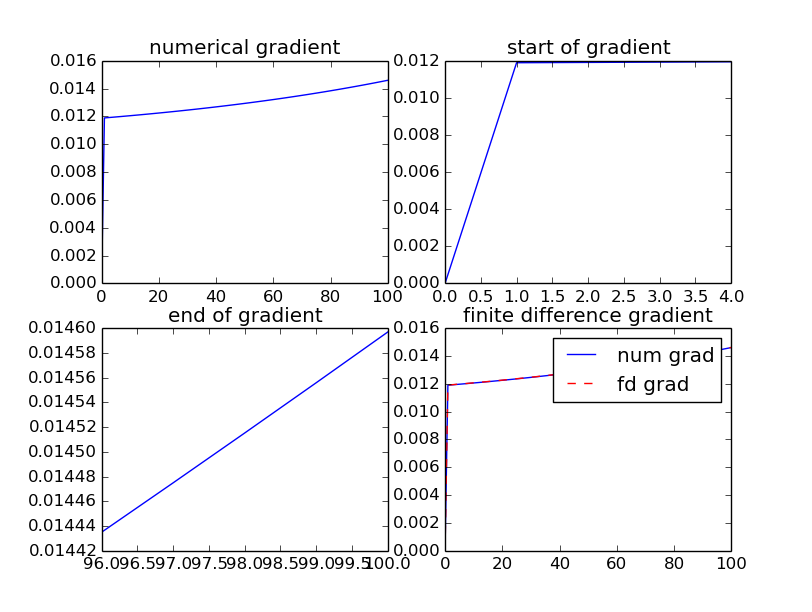
\includegraphics[scale=0.5]{num_grad.png}
\end{figure}
\subsection{Verifying the penalized numerical gradient using the Taylor test}
We will now use the Taylor test on the penalized numerical gradient (\ref{num_pen_grad_lam}-\ref{num_pen_grad_v}) that we get when decomposing $I=[0,T]$ into $N=10$ subintervals while solving the same problem as in the test for the gradient of the non-penalized objective function (\ref{test_J}-\ref{test_E}). We then discretize in time using $\Delta t=\frac{1}{100}$. The control variable is now a vector $v\in\mathbb{R}^{N+m}$ and we set $v_k=0 \ \forall k=0,...,N+n-1$, while the $w_k$s are chosen randomly from numbers between 0 and 100. The results of applying the Taylor test to this problem are given in table \ref{Taylor_tab2}. Here $D_1$ and $D_2$ are again defined as in (\ref{D1}-\ref{D2}).
\\
\begin{table}[!h]
\caption{Taylor test}
\centering
\label{Taylor_tab2}
\begin{tabular}{lrrrll}
\toprule
{}$\epsilon$&  $D_1$ &  $D_2$ &        $||\epsilon w||_{l_{\infty}}$ &    $ \log(\frac{D_1(10\epsilon)}{D_1(\epsilon)})$ &    $ \log(\frac{D_2(10\epsilon)}{D_2(\epsilon)})$  \\
\midrule
1.000000e+00 &  1.080513e+04 &        1.076907e+04 &  9.771288e+01 &       -- &       -- \\
1.000000e-01 &  1.112972e+02 &        1.076907e+02 &  9.771288e+00 &  1.98715 &        2 \\
1.000000e-02 &  1.437558e+00 &        1.076907e+00 &  9.771288e-01 &  1.88886 &        2 \\
1.000000e-03 &  4.683423e-02 &        1.076907e-02 &  9.771288e-02 &  1.48706 &        2 \\
1.000000e-04 &  3.714207e-03 &        1.076907e-04 &  9.771288e-03 &   1.1007 &        2 \\
1.000000e-05 &  3.617285e-04 &        1.076907e-06 &  9.771288e-04 &  1.01148 &        2 \\
1.000000e-06 &  3.607593e-05 &        1.076908e-08 &  9.771288e-05 &  1.00117 &        2 \\
1.000000e-07 &  3.606624e-06 &        1.076979e-10 &  9.771288e-06 &  1.00012 &  1.99997 \\
1.000000e-08 &  3.606527e-07 &        1.086074e-12 &  9.771288e-07 &  1.00001 &  1.99635 \\
\bottomrule
\end{tabular}
\end{table}
\\
\\
Again we see that $|J(v+\epsilon w)-J(v)-\epsilon \nabla J(v)\cdot w|$ converges to zero at a second order rate, meaning that the penalized numerical gradient also passes the Taylor test.
\begin{figure}[h]
\caption{Plots showing the $\Lambda$ and control part of the numerical gradient found using formula (\ref{num_pen_grad_lam}-\ref{num_pen_grad_v}) and finite difference}
\centering
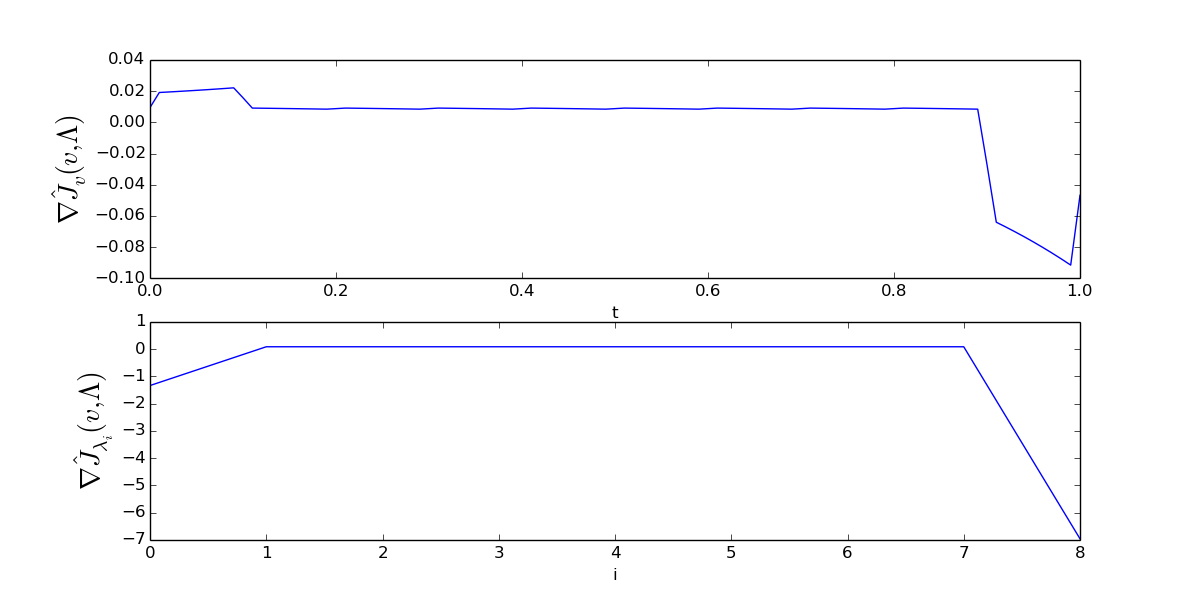
\includegraphics[scale=0.5]{pen_num_grad.png}
\end{figure}
\section{Convergence rate of solver for the non-penalized problem}
In section \ref{Taylor_sec} we demonstrated that our implementation of the gradients for different discretizations of the objective function introduced in theorem \ref{Theorem_num_grad} and \ref{Theorem_penalty_grad} satisfy the Taylor test. Since the discretized objective function $\hat J_{\Delta t}$ and its gradient pass the Taylor test, we expect that we can find the minimizer $\bar v$ of $\hat J_{\Delta t}$ by using an optimization algorithm. What we now want to find out, is if the minimizer of the discrete objective function converges towards the exact minimizer derived in section \ref{exact_sec}. We investigate this by solving optimal control problem (OBS! OBS!) using both a Crank-Nicolson and an implicit Euler discretization. To measure the difference between exact optimal control $v_e$ and the numerical optimal control $v$ we look at the relative maximal difference between $v_e$ and $v$ for $t\in(0,T)$, meaning
\begin{align}
||v|| = \max_{k=1,...,n-1}|v_k| \label{inner_norm}
\end{align} 
We also look at the relative difference in objective function value between the controls. For both these measures, we calculate at what rate they converge to zero for decreasing $\Delta t$ values. The results for the implicit Euler discirization is found in table \ref{IE_convergence}, while Crank-Nicolson results are given in table \ref{CN_convergence}.
\begin{table}[h]
\caption{Convergence of implicit Euler numerical sequential solver of optimal control problem.}\label{IE_convergence}
\centering
\begin{tabular}{lrrll}
\toprule
{} $\Delta t$&    $\frac{||v_e-v||}{||v||}$ &  $\frac{\hat J(v_e)-\hat J(v)}{\hat J(v_e)}$ &   norm rate &    functional rate \\
\midrule
0.02000 &  0.212619 &  1.709101e-02 &        -- &       -- \\
0.01000 &  0.136096 &  4.506561e-03 & -0.643642 & -1.92314 \\
0.00100 &  0.017469 &  4.703915e-05 & -0.891585 & -1.98139 \\
0.00010 &  0.001795 &  4.722900e-07 &   -0.9883 & -1.99825 \\
0.00001 &  0.000180 &  4.724790e-09 &  -0.99882 & -1.99983 \\
\bottomrule
\end{tabular}
\end{table}
Notice that the convergence rate of the norm difference in table \ref{IE_convergence} approaches one when $\Delta t$ tends to zero. This is consistent with what we would expect for a finite difference scheme of first order. We also notice that the difference in function value converges an order of one faster towards zero than the control difference.  
\begin{table}[h]
\caption{Convergence of Crank-Nicolson numerical sequential solver of optimal control problem.}\label{CN_convergence}
\centering
\begin{tabular}{lrrll}
\toprule
{} $\Delta t$&    $\frac{||v_e-v||}{||v||}$ &  $\frac{\hat J(v_e)-\hat J(v)}{\hat J(v_e)}$ &   norm r &    val r \\
\midrule
0.02000 &  4.177702e-02 &  2.309886e-03 &       -- &       -- \\
0.01000 &  1.109500e-02 &  3.383020e-04 &  -1.9128 & -2.77144 \\
0.00100 &  1.189515e-04 &  3.931451e-07 & -1.96976 & -2.93475 \\
0.00010 &  1.421834e-06 &  3.992950e-10 & -1.92252 & -2.99326 \\
0.00001 &  1.480190e-08 &  3.978299e-13 & -1.98253 &  -3.0016 \\
\bottomrule
\end{tabular}
\end{table}
The results of table \ref{CN_convergence} show results similar to the ones in table \ref{IE_convergence}, however the convergence rates using a Crank-Nicolson scheme to discretize the ODEs are one order higher than the rates we got using implicit Euler. This is again expected since the Crank-Nicolson scheme is of order two. In both tables we observe that $\frac{\hat J(v_e)-\hat J(v)}{\hat J(v)}$ is always positive, which means that $\hat J(v_e)>\hat J(v)$. This makes sense, since $\hat J$ here means the discrete objective function, and $v$ is the minimum of this function, while $v_e$ is the minimum of the continuous objective function. One last remark concerns the choice of norm (\ref{inner_norm}). This norm excludes the values of $v$ and $v_e$ at $t=0$ and $t=T$. If these points are included, we do not see the convergence rates given in table \ref{IE_convergence} and \ref{CN_convergence}. 
\section{Verifying function and gradient evaluation speedups} \label{ver S sec}
In \ref{analysis sec} we derived the theoretical speedup for numerical gradient and objective function evaluation when decomposing the time-interval. It would now be interesting to check if the implementation achieves the theoretical speedup for our example problem. The specific problem is:
\begin{align*}
&J(y,v) = \frac{1}{2}\int_0^1v(t)^2dt + \frac{1}{2}(y(T)-1)^2 \\
&\left\{
     \begin{array}{lr}
       	y'(t)+y(t) = v(t) \ t\in(0,1)\\
       	y(0)=1
     \end{array}
   \right. 
\end{align*}
A computer with 6 cores was used to verify the results of section \ref{analysis sec}. Having 6 cores means that we can do gradient and function evaluation for $N=1,2,...,6$ decompositions with different time step sizes $\Delta t$. For each combination of $N$ and $\Delta t$, we will run the function and gradient evaluations ten times, and then choose the the smallest execution time produced by the ten runs. The speedup is then calculated by dividing the sequential execution time by the parallel execution time. Tables \ref{Speed_table1}-\ref{speed_table_end} below shows runtime and speedup for both gradient and function evaluation for different $\Delta t$s and $N$s. All evaluations are done with control input $v=1$ and $\lambda_i=1$.  
\\
\begin{table}[!h]
\centering
\caption{$\Delta t=10^{-2}$}
\label{Speed_table1}
\begin{tabular}{lrr}
\toprule
{} $N$&   function speedup &      function time \\
\midrule
1 &  1.000000 &  0.000196 \\
2 &  0.946860 &  0.000207 \\
3 &  0.780876 &  0.000251 \\
4 &  0.642623 &  0.000305 \\
5 &  0.544444 &  0.000360 \\
6 &  0.427948 &  0.000458 \\
\bottomrule
\end{tabular}
\begin{tabular}{lrr}
\toprule
{} &  gradient speedup &     gradient time \\
\midrule
1 &  1.000000 &  0.000217 \\
2 &  0.875000 &  0.000248 \\
3 &  0.753472 &  0.000288 \\
4 &  0.632653 &  0.000343 \\
5 &  0.547980 &  0.000396 \\
6 &  0.480088 &  0.000452 \\
\bottomrule
\end{tabular}
\end{table}
\begin{table}[!h]
\centering
\caption{$\Delta t=10^{-4}$}
\begin{tabular}{lrr}
\toprule
{} $N$&  function speedup &    function  time \\
\midrule
1 &  1.000000 &  0.008877 \\
2 &  1.983687 &  0.004475 \\
3 &  2.838823 &  0.003127 \\
4 &  3.582324 &  0.002478 \\
5 &  4.267788 &  0.002080 \\
6 &  4.519857 &  0.001964 \\
\bottomrule
\end{tabular}
\begin{tabular}{lrr}
\toprule
{} &  gradient speedup &     gradient time \\
\midrule
1 &  1.000000 &  0.015016 \\
2 &  1.946843 &  0.007713 \\
3 &  2.816204 &  0.005332 \\
4 &  3.677688 &  0.004083 \\
5 &  4.457109 &  0.003369 \\
6 &  4.978780 &  0.003016 \\
\bottomrule
\end{tabular}
\end{table}
\begin{table}[!h]
\centering
\caption{$\Delta t=10^{-5}$}
\begin{tabular}{lrr}
\toprule
{}$N$ &  function speedup &    function  time \\
\midrule
1 &  1.000000 &  0.087484 \\
2 &  2.006606 &  0.043598 \\
3 &  2.888595 &  0.030286 \\
4 &  3.913222 &  0.022356 \\
5 &  4.848102 &  0.018045 \\
6 &  5.425028 &  0.016126 \\
\bottomrule
\end{tabular}
\begin{tabular}{lrr}
\toprule
{} &  gradient speedup &     gradient time \\
\midrule
1 &  1.000000 &  0.154841 \\
2 &  2.046537 &  0.075660 \\
3 &  2.971198 &  0.052114 \\
4 &  4.003025 &  0.038681 \\
5 &  4.921368 &  0.031463 \\
6 &  5.755101 &  0.026905 \\
\bottomrule
\end{tabular}
\end{table}
\begin{table}[!h]
\centering
\caption{$\Delta t=10^{-7}$}
\label{speed_table_end}
\begin{tabular}{lrr}
\toprule
{}$N$ &  function speedup &      time \\
\midrule
1 &  1.000000 &  8.350907 \\
2 &  1.987960 &  4.200743 \\
3 &  2.847662 &  2.932549 \\
4 &  3.812545 &  2.190376 \\
5 &  4.647839 &  1.796729 \\
6 &  5.479447 &  1.524042 \\
\bottomrule
\end{tabular}
\begin{tabular}{lrr}
\toprule
{} &  gradient speedup &     gradient  time \\
\midrule
1 &  1.000000 &  14.930247 \\
2 &  2.064043 &   7.233497 \\
3 &  2.966254 &   5.033368 \\
4 &  3.866428 &   3.861509 \\
5 &  4.833081 &   3.089178 \\
6 &  5.744552 &   2.599027 \\
\bottomrule
\end{tabular}
\end{table}
\\
\\
Since the parallel algorithm has some overhead, we do not expect any improvements for small problems. This is reflected in the above results, where we for $\Delta t = 10^{-2}$ see an increased execution time when running function and gradient evaluation in parallel. For $\Delta t = 10^{-4}$ we see only a modest speedup, that is significantly lower than the expected speedup from section \ref{analysis sec}. For $\Delta t \leq 10^{-5}$, however we see speedup results in line with what we expect from the theory.  
\section{Consistency}
When we introduced the penalty method in section \ref{penalty_sec}, we also presented a result showing that the iterates $\{v^k\}$ stemming from the penalty algorithmic framework converged towards the solution of the non-penalized problem $v$. We can write this up as:
\begin{align*}
\lim_{k\rightarrow\infty} v^k = v 
\end{align*}  
An alternative way of looking at this, is to let $v^{\mu}$ be the minimizer of $\hat J_{\mu}$, and instead write the above limit as:
\begin{align}
\lim_{\mu\rightarrow\infty} v^{\mu} = v \label{mu con}
\end{align}
The interpretation of the above limit, is that solving the penalized problem with an ever increasing penalty parameter $\mu$ should result in a solution that is getting closer and closer to the solution of the non-penalized problem. This means that the penalty algorithm is consistent, since it produces the same solution as the ordinary non-decomposed problem. It is therefore worth checking if the implementation of the penalized problem actually has the property (\ref{mu con}). The particular problem, that we will do the consistency test on, is: 
\begin{align}
&J(y,v) = \frac{1}{2}\int_0^1v(t)^2dt + \frac{1}{2}(y(T)-11.5)^2 \label{con J} \\
&\left\{
     \begin{array}{lr}
       	y'(t)=-3.9y(t) + v(t) \ t\in(0,1)\\
       	y(0)=3.2
     \end{array}
   \right. \label{con E}
\end{align}
We want to compare the solution we get by decomposing and then applying the penalty method on problem (\ref{con J}-\ref{con E}) with the solution we get by solving the undecomposed problem. To do this we discretize (\ref{con J}-\ref{con E}) using two different time steps. First we let $\Delta t = 10^{-2}$ and apply the penalty method for $N=2$ and $N=10$ decompositions, we then let $\Delta t = 10^{-3}$ and test the penalty method on $N=2$ and $N=7$ decompositions. For both time steps, the Crank-Nicolson will be used to discretize the state and adjoint equations. We use different metrics to compare the non-penalized and penalized solutions, so that we better see how the solution of the penalized problem behaves when we solve it for an increasing sequence of $\mu$ values. We define the metrics as follows:
\begin{align*}
\textrm{Realtive objective function differnce:}\quad A &= \frac{\hat{J}(v_{\mu})-\hat{J}(v)}{\hat{J}(v)}\\
\textrm{Realtive penalized objective function differnce:}\quad B &= \frac{\hat{J}_{\mu}(v)-\hat{J}_{\mu}(v_{\mu})}{\hat{J}_{\mu}(v)}\\
\textrm{Relative control $L^2$-norm difference:}\quad C&=\frac{||v_{\mu}-v||_ {L^2}}{||v||_{L^2}} \\
\textrm{Maximal jump in decomposed state equation:}\quad D&= \sup_i\{y_{k_i}^i-y_{k_i}^{i+1}\}\\
\end{align*}
Notice that both $A$ and $B$ should be grater than $0$, since $v$ and $v_{\mu}$ are the minimizers of $\hat J$ and $\hat J_ {\mu}$. The measure of jumps in the state equation $D$ is added to check that the penalty solution approaches a feasible solution in context of the continuity constraints (\ref{Extra constraints}). The results of the above detailed experiment are presented through logarithmic plots in figure \ref{Cons1_fig} and \ref{Cons2_fig}. 
\\
\\
\begin{figure}[!h]
\centering
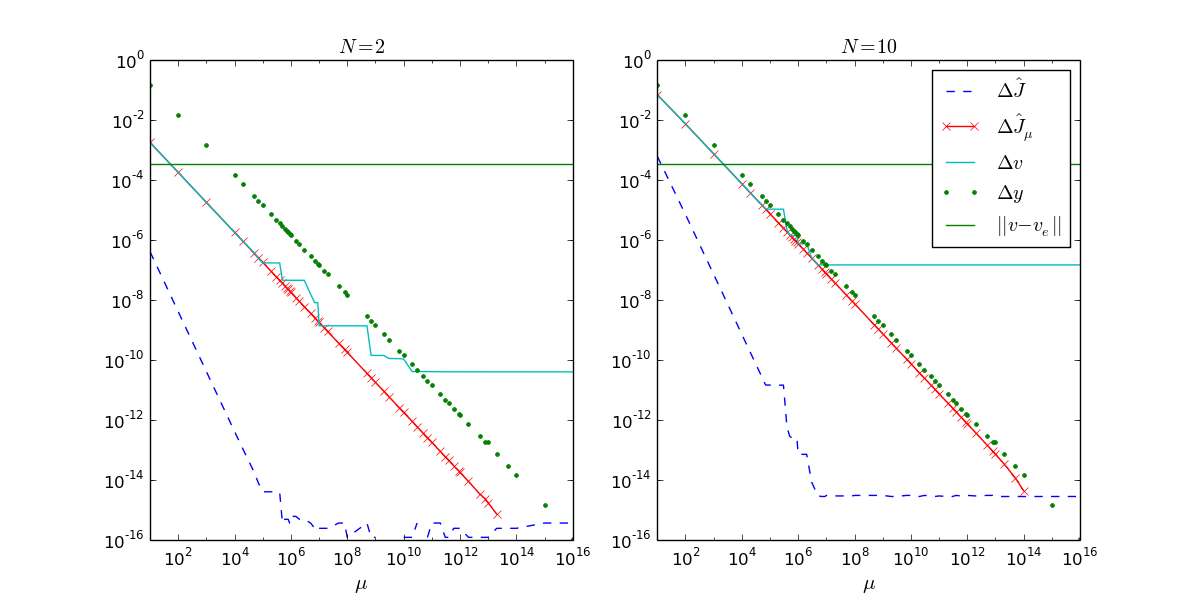
\includegraphics[scale=0.5]{consistency1.png}
\caption{Logarithmic plot showing how solution of penalty method applied to problem (\ref{con J}-\ref{con E}) develops for $\Delta t = 10^{-2}$.}
\label{Cons1_fig}
\end{figure}
\begin{figure}[!h]
\centering
\includegraphics[scale=0.5]{consistency2.png}
\caption{Same as figure \ref{Cons1_fig}, only now $\Delta t = 10^{-3}$.}
\label{Cons2_fig}
\end{figure}
The plots in figure \ref{Cons1_fig} and \ref{Cons2_fig} all show a similar picture, and we observe that all measures decrease when the penalty parameter is increased. Still there are several parts of the plots worthy of note. The measure $A$ related to the unpenalised objective function is the value that converges to zero the fastest. If we look at the vales of $A$ before the machine precision is reached we see that $A$ is proportional to $\frac{C}{\mu^2}$. The convergence rate of $A$ for $\Delta t=10^{-2}$ and $N=2$ is shown in table \ref{Cosn_rate_table} together with the rate convergence rate of $C$. $C$ and the other measures converge to zero at a rate of one, however we see that the relative error between the controls $v$ and $v_{\mu}$ $C$ stops to decrease long before the machine precision is reached. It seems that this barrier is hit around the same time as $A$ approaches machine precision. The reason for this probably is that small changes in the control $v_{\mu}$ no longer registers in $\hat J_{\mu}$, and it is therefore difficult to find an appropriate step length in the line search method.
\\
\\
$B$ and $D$ on the other hand continue to decrease steadily towards zero, even after $A$ has hit machine precision. The $B$ and $C$ metrics are both related to the $\frac{\mu }{2}\sum_{i=1}^{N-1}(y^i(T_{i})-\lambda_i)^2$ term, which is the part that enforces the continuity constraints (\ref{Extra constraints}). This means that after a certain point, the penalty method only improves the $\Lambda$ part of the control, while $v$ remains the same. 
\begin{table}[!h]
\centering
\caption{Convergence rates for $\Delta t=10^{-2}$ and $N=2$. Notice how the $||v_{\mu}-v||$ stops to decrease at around the same time as $\frac{J(v_{\mu})-J(v)}{J(v)}$ hits machine precision.}
\label{Cosn_rate_table}
\begin{tabular}{lrrll}
\toprule
{} $\mu$&  $\frac{J(v_{\mu})-J(v)}{J(v)}$ &   $||v_{\mu}-v||$ &        A rate &        C rate \\
\midrule
1.000000e+01 &      4.105697e-07 & 1.790231e-03 &            -- &            -- \\
1.000000e+02 &      4.119052e-09 & 1.793140e-04 & -1.998590 & -0.9992948 \\
1.000000e+03 &      4.120272e-11 & 1.793401e-05 & -1.999871 & -0.9999368 \\
1.000000e+04 &      4.137632e-13 & 1.796793e-06 & -1.998174 & -0.9991795 \\
2.000000e+04 &      1.058008e-13 & 9.076756e-07 & -1.967455 & -0.9851756 \\
5.000000e+04 &      1.789909e-14 & 3.733858e-07 & -1.939131 & -0.9694245 \\
7.000000e+04 &      7.968773e-15 & 2.444327e-07 & -2.405011 & -1.259160 \\
1.000000e+05 &      4.045685e-15 & 1.730018e-07 & -1.900553 & -0.9690555 \\
2.000000e+05 &      4.045685e-15 & 1.721746e-07 &  0.000000 & -0.0069153 \\
3.000000e+05 &      3.923088e-15 & 1.719606e-07 & -0.007589 & -0.0030671 \\
4.000000e+05 &      3.800492e-15 & 1.718652e-07 & -0.110360 & -0.0019278 \\
5.000000e+05 &      3.677895e-16 & 4.545076e-08 & -10.46580 & -5.960652e \\
\bottomrule
\end{tabular}

\end{table}

\chapter{Experiments}\label{Experiments chapter}
In this chapter we will through experiments investigate what speedup one might get by using the algorithm for parallelizing optimal control problems with  time dependent DE constraints in temporal direction, introduced in previous chapters. Unlike the parallel performance of gradient and objective function evaluation, the parallel performance of our overall algorithm is difficult to model. The reason for this is that it is difficult to say how many gradient and function evaluations are needed for the optimization algorithms to terminate. We are therefore unable to derive any theoretical expected speedup.
\\
\\
In section \ref{analysis sec} we explained that the best way of measuring performance of a parallel algorithm is to compare its execution time to the sequential execution time of the best sequential algorithm. When solving optimal control problems with DE constraints, the runtime of our solution algorithm will depend on how many times we have to evaluate the objective function and its gradient, since these evaluations require either the solution of the state equation or the state and adjoint equations. We know from theory in section \ref{analysis sec} and verification in section \ref{ver S sec}, that the speedup of parallel gradient and function evaluation depends linearly on the number of processes we use. An alternative way of measuring parallel performance is therefore to compare the sum of gradient and function evaluations in the sequential and parallel algorithms. Let us give this numbers a name:
\begin{align*}
L_s &= \textit{Number of function and gradient evaluations for sequantial algorithm}\\
L_{p_N} &= \textit{Number of function and gradient evaluations for parallel algorithm using N processes}
\end{align*} 
Using these definitions we define the ideal speedup $\hat{S}$, as the speedup one would expect based on $L_s$ and $L_{p_N}$ and the speedup results we have for function and gradient evaluations:
\begin{align}
\hat S = \frac{NL_s}{L_{p_N}} \label{ideal S}
\end{align}
With $\hat S$, it is possible to say something about the performance of the parallel algorithm without having to time it, or actually run it in parallel. It will also be useful to compare the ideal speedup with the measured speedup, as a way to check if the parallel implementation is implemented efficiently.
\section{Testing Parareal-based preconditioner on example problem}
In this section we will test the parallel framework introduced in chapter \ref{method_chap} on our example problem (\ref{exs_J}-\ref{exs_E}). To be able to do this, we need to define a specific objective function and state equation. The problem we will look at in this section is the following:
\begin{align}
&J(y,v) = \frac{1}{2}\int_0^{T}v(t)^2dt + \frac{1}{2}(y(T)-11.5)^2,\quad T=100, \label{speed_j}\\
&\left\{
     \begin{array}{lr}
       	y'(t)=-0.097y(t) + v(t) \quad t\in(0,T)\\
       	y(0)=3.2
     \end{array}
   \right. \label{speed_e}
\end{align}
We motivate the choice of a large end time $T=100$ with the findings of section \ref{consistency_sec}. There we observed that the penalty method ran into trouble when the time steps became too small, because the error in objective function value then hit machine precision. To be able to test the problem for a large number of time steps, we therefore need a large $T$. 
\subsection{Comparing unpreconditioned and preconditioned penalty framework}
In section \ref{pc sec} we introduced the parareal preconditioner, as an approximation to the Hessian. Using this preconditioner in our L-BFGS solver we hope that the number of gradient and function evaluations needed in our algorithm will be smaller than if we do not use it. The experiment is conducted by first solving this problem without decomposing the time interval, and then solving the decomposed problem using $N=2,4,8,16,32,64,128$ decompositions. For all minimizations of the penalized objective function, we used penalty parameter $\mu=10^4$. This means that we will only use one penalty iteration, as we have found this to be the most effective way to solve the decomposed problem for this specific problem. To discretize the equations we have used the Crank-Nicolson scheme with $\Delta t= \frac{T}{1000}=0.1$. For both the penalized and non-penalized problems we use L-BFGS with stop criteria:
\begin{align*}
||\nabla J||_{L^2} <10^{-5}
\end{align*}  
Since the point of this test is to compare the effectiveness of the Parareal-based preconditioner, we solve the decomposed problems with and without it. In table \ref{speed1} we have included the total number of gradient and function evaluations for the two cases as "pc L" and "non-pc L". We also measured the relative $L^2$-norm difference between the exact solution $v_e$ and all the penalized control solutions. The ideal speedup (\ref{ideal S}) is calculated for preconditioned and unpreconditioned solvers.
\\
\\
\begin{table}[h]
\centering
\caption{Comparing unpreconditioned and preconditioned solver for test problem (\ref{speed_j}-\ref{speed_e}) using $N$ decompositions in time. Here $v_e$ denotes the exact control solution, $v_{pc}$ the preconditioned solver control solution and $v$ the unpreconditioned solver solution. $L_{p_N}$ represents total number of gradient and function evaluations used in each optimization. The ideal speedup $\hat S$ is based on this $L_{p_N}$. Notice that the preconditioned ideal speedup is significantly larger than the unpreconditioned ideal speedup for large $N$.}
\label{compare_table}
\begin{tabular}{lrrllrr}
\toprule
{}$N$ &  pc $L_{p_N}$ &  non-pc $L_{p_N}$ &       $||v_e-v_{pc}||$ &  $||v_e-v||$  &  pc $\hat{S}$ &  non-pc $\hat{S}$ \\
\midrule
1   &     19 &      19 &  0.000174 &    0.000174 &    1.000 &        1.000 \\
2   &     21 &      21 &  0.001093 &    0.001093 &    1.809 &        1.809 \\
4   &     45 &      45 &  0.000640 &    0.000361 &    1.688 &        1.688 \\
8   &     61 &      69 &  0.000667 &    0.001590 &    2.491 &        2.202 \\
16  &     61 &     241 &  0.001608 &    0.000784 &    4.983 &        1.261 \\
32  &     73 &     343 &  0.001909 &    0.002528 &    8.328 &        1.772 \\
64  &     67 &     737 &  0.005273 &    0.004816 &   18.149 &        1.649 \\
128 &     67 &     907 &  0.010892 &    0.018467 &   36.298 &        2.681 \\
\bottomrule
\end{tabular}
\end{table}
\\
\\
There are several things of note about the results in table \ref{compare_table}. First off we see that the normed difference in control between exact and parallel solution lies in the range from $10^{-4}$ to $10^{-2}$. Another observation about the norm difference, is that for each $N$, the preconditioned and unpreconditioned solvers seems to produce roughly the same error. 
\\
\\
When we look at the total number of gradient and functional evaluations for the preconditioned and unpreconditioned solvers, we see that there are differences. While it seems to be little to no benefit to use the preconditioner for $N=1,...,8$, it becomes very important for the bigger $N$ values, where number of gradient and functional evaluations seems to explode for the unpreconditioned solver. If one accepts the above solutions as good enough, we see that we for the preconditioned solver get speedup for all decompositions, and that the ideal speedup seems to increase when we increase $N$. We do however see that the ideal speedup for each $N$ is considerably less then optimal for all $N$. Another thing that we notice when looking at the sum of gradient and function evaluations for the preconditioned solver, is that it increases steadily up to $N=8$, and then starts to decline again for higher $N$s. The reason for this is that when we increase the number of decomposed subintervals, we also make the coarse solver in the parareal preconditioner finer. This means that the preconditioner becomes a better approximation of the Hessian, which makes the L-BFGS iteration converge faster.
\subsection{Speedup results for a high number of decompositions} \label{Aspeed_sec}
To properly test the Parareal-based preconditioner, we have tested its use on the example problem on the Abel computer cluster. Using Abel, we are able to test our algorithm for a large number of CPUs. For all experiments the execution time of the sequential parallel algorithms is measured by timing the solvers ten times, and choosing the lowest execution time. All our tests are done using an implicit Euler discretization. We run the test for three different problem sizes $n=6\cdot 10^5,12\cdot 10^5,24\cdot 10^5$ using an increasing number of processes $N$. Each process gets its own decomposed subinterval. The results for selected values of $N$ and $n= 24\cdot 10^5$ is found in table \ref{speed1}, while the remaining results are presented in figure \ref{speed_fig1}.
\\
\begin{table}[h]
\centering
\caption{Results gained form solving problem (\ref{speed_j}-\ref{speed_e}) for $n=24\cdot 10^5$ on $N$ processes. The first two columns shows the error in control and objective function value. $L_{p_N}$ is the total number of gradient and function evaluations, while $\hat S$ is the ideal speedup. The execution time for each $N$, and the corresponding speedup and efficiency are given in the last three columns.}
\label{speed1}
\begin{tabular}{lrlrrrrr}
\toprule
{}$N$ &   $\frac{||v-v_e||_{L^2}}{||v_e||_{L^2}}$ &     $\frac{\hat J(v)-\hat J(v_e)}{\hat{J}(v_e)}$ &   $L_{p_N}$ &     $\hat S$ &       time (s) &    speedup &        efficiency \\
\midrule
1   &  0.000002 &           -- &  19 &   1.000 &  63.370 &   1.000 &  1.0000 \\
4   &  0.000018 &  2.761e-10 &  37 &   2.054 &  40.124 &   1.579 &  0.3948 \\
16  &  0.000061 &  3.169e-09 &  97 &   3.134 &  28.409 &   2.230 &  0.1394 \\
32  &  0.000044 &   1.65e-09 &  85 &   7.152 &  12.681 &   4.997 &  0.1561 \\
48  &  0.000031 &  8.285e-10 &  73 &  12.493 &   7.056 &   8.980 &  0.1871 \\
72  &  0.000021 &  3.703e-10 &  88 &  15.545 &   6.243 &  10.149 &  0.1409 \\
96  &  0.000015 &  2.196e-10 &  61 &  29.901 &   3.630 &  17.452 &  0.1817 \\
120 &  0.000012 &  1.727e-10 &  61 &  37.377 &   2.690 &  23.556 &  0.1963 \\
\bottomrule
\end{tabular}
\end{table}
\noindent
\\
The results of table \ref{speed1} shows that our parallel method can achieve actual speedup. The achieved speedup is however quite modest, since we for 120 cores only get a speedup of $23.5$. We also notice that the speedup is smaller then the ideal speedup $\hat S$. This is as expected, since $\hat S$ assumes zero parallel overhead. There are three factors that cause the parallel overhead. The first is the overhead caused by communication and hardware. It is difficult to diminish these effects, but when the problem size increase the impact of the built in overhead should decrease. The second factor is our implementation. Our code is not optimized, and has a bigger effect on the more complicated parallel algorithm than the sequential one. The effects of a suboptimal implementation does not necessarily diminish when we increase the problem size, but we might be able to remove these effects by improving our code. The last factor that impacts the parallel overhead, is our sequential Parareal-based preconditioner. The Parareal-based preconditioner is applied to the gradient through a backward and a forward solve on a coarse mesh of size $N$. This means that the effect of preconditioner on the parallel overhead increases when we increase the numbers of processes. If $N<<n$ these effects will however be very small. The results of table \ref{speed1} are by found solving a problem of size $n=24\cdot 10^5$, while the largest $N$ value is $120$, which means that N is $20000$ times smaller than $n$. It is therefore unlikely that it is the sequential Parareal-based preconditioner that is the main cause of the gap between ideal and measured speedup in table \ref{speed1}. Instead the disparity in ideal and measured speedup is probably caused by a combination built in overhead and a suboptimal implementation.
\\
\\
Another interesting observation about table \ref{speed1}, is that the solution seems to improve when we increase $N$, which we see by looking at how the numerical control solution compares to the exact solution when we increase $N$. We compare exact and numerical solution by looking at normed difference in control and difference in function value. For $N\leq16$ these measures increase, but for $N>16$ they start to decrease again. We see the same type of pattern for $L_{p_N}$, which represents the total number of objective function and gradient evaluations done in each optimization. One interpretation of this, is that the Parareal-based preconditioner improves when the coarse decompositions become finer. The results of figure \ref{speed_fig1} paints a similar picture.
\begin{figure}[!h]
\centering
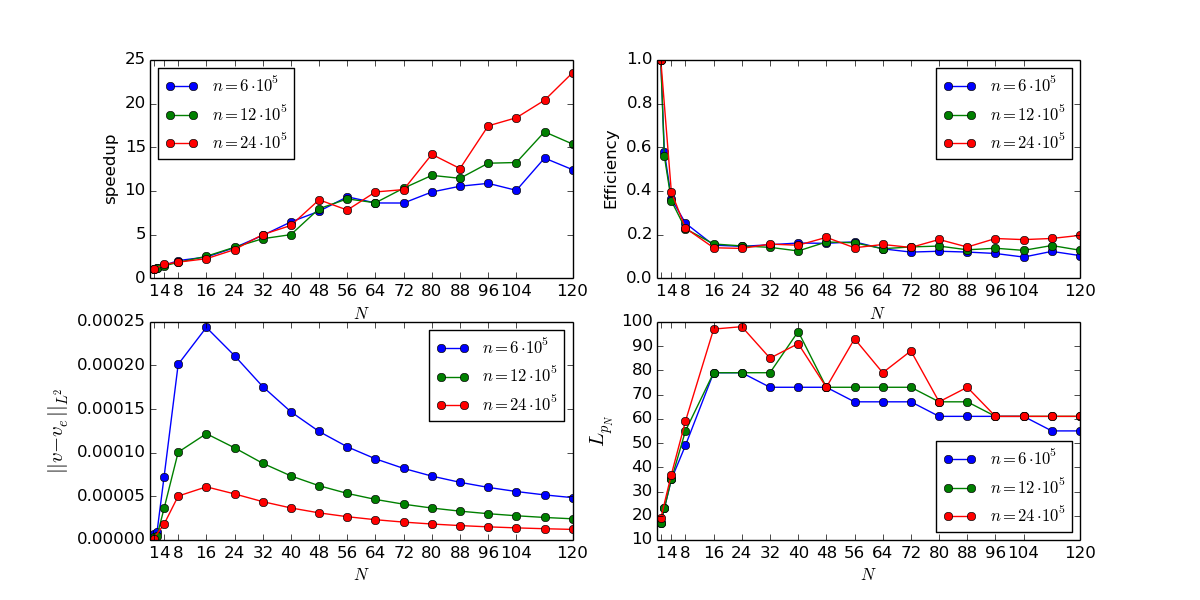
\includegraphics[scale=0.5]{fspeed_fig.png}
\centering
\caption{Speedup, efficiency, relative norm error and total number of objective function and gradient evaluations  ($L_{p_N}$) for problem (\ref{speed_j}-\ref{speed_e}) solved using $n=6\cdot 10^5,12\cdot 10^5,24\cdot 10^5$ time steps on $N$ cores.}
\label{speed_fig1}
\end{figure}
\\
\\
By looking at figure \ref{speed_fig1}, we see that our algorithm preformed the best, at least in the sense of speedup, for $n=24\cdot 10^5$. We do however also observe the same type of behaviour for all values of $n$. We see that the error between exact and numerical control solution for all $n$ first increases up till around $N=16$, and then decreases and flattens out. The total number of gradient and function evaluations $L_{p_N}$ becomes larger for higher $N$s when $N\leq 16$, but for $N>16$ $L_{p_N}$ starts to decrease slightly. 
\subsection{Tests on a less smooth problem}
As we see by looking at figure \ref{smootha}, the control solution of our example problem (\ref{speed_j}-\ref{speed_e}), is very smooth. It is therefore interesting to see if our algorithm is produce good results for problems with more uneven solutions. A simple way of slightly complicating our example problem is to add a sine function to the integral in the objective function. To produce the control solution pictured in \ref{smoothb}, we alter $J$ in the following way:
\begin{align}
J(y,v) = \frac{1}{2}\int_0^{T}(v(t)-0.3\sin(t))^2dt + \frac{1}{2}(y(T)-11.5)^2, \quad T=100. \label{sinJ}
\end{align}
We will now try to minimize the altered objective function (\ref{sinJ}) with same state equation constraints as before, using our algorithm. Since we in section \ref{Aspeed_sec} showed that our algorithm is capable of producing actual speedup, we are now only looking at ideal speedup and not wall clock speedup. In table \ref{unsmoothTab} we present results gained by applying our algorithmic framework to a Crank-Nicholson discretized minimization of the altered objective function (\ref{sinJ}) using $\Delta t = 10^{-2}$.
\begin{figure}[h]
\centering
\begin{subfigure}{.5\textwidth}
  \centering
  \includegraphics[width=.8\linewidth]{smooth.png}
  \caption{Minimizer of objective function (\ref{speed_j})}
  \label{smootha}
\end{subfigure}%
\begin{subfigure}{.5\textwidth}
  \centering
  \includegraphics[width=.8\linewidth]{unsmooth.png}
  \caption{Minimizer of objective function (\ref{sinJ})}
  \label{smoothb}
\end{subfigure}
\caption{Optimal control for the unaltered and altered example problem (\ref{speed_j}-\ref{speed_e}). Notice the smoothness and simplicity of figure \ref{smootha}.}
\label{smooth}
\end{figure}
\begin{table}
\caption{Results of applying our algorithmic framework to optimization of (\ref{sinJ}) for different decomposition sizes $N$. The columns display error ($\frac{||v-v_{\mu}||}{||v||}$), total number of gradient and function evaluations ($L_{p_N}$) and ideal speedup ($\hat S$).}
\centering
\label{unsmoothTab}
\begin{tabular}{lrrr}
\toprule
{} $N$&   $\frac{||v-v_{\mu}||}{||v||}$ &  $L_{p_N}$ &     $\hat S$ \\
\midrule
1   &  0.000000 &   67 &   1.000 \\
2   &  0.000060 &  101 &   1.326 \\
4   &  0.000029 &  143 &   1.874 \\
8   &  0.000002 &  127 &   4.220 \\
16  &  0.000028 &  139 &   7.712 \\
32  &  0.000008 &  193 &  11.108 \\
64  &  0.000042 &  193 &  22.217 \\
128 &  0.000009 &  201 &  42.666 \\
\bottomrule
\end{tabular}
\end{table}
It is interesting to contrast the findings of table \ref{unsmoothTab} with the results from table \ref{compare_table}. We notice that the total number of gradient and function evaluations ($L_{p_N}$) is consistently higher in table \ref{unsmoothTab}, but since this is also the case for the sequential solver, we actually observe better ideal speedup in table \ref{unsmoothTab} than in table \ref{compare_table}. This might indicate that our method has a higher potential for success on more complicated problems, where the serial solver requires a higher number function and gradient evaluations.
\chapter{Summary and Conclusions} \label{summary chap}
The topic of this thesis is the parallelization of optimization problems with time-dependent differential equation constraints. The method we have proposed is developed around reducible problems, where the state equation constraint is well posed and time-dependent. Our method has been explained through a simple ODE constrained example problem, and we have also used this example for verification and testing. Even though we only considered an ODE example, we believe that our method also is applicable to time-dependent PDE constrained problems. Examples of such constraints can be PDEs on form (\ref{PDE_exs}).
\begin{align}
\left\{
     \begin{array}{lr}
       	u_t(x,t) + Au(x,t)=f \quad \textrm{for } \ (x,t)\in U\times(0,T),\\
       	u(x,0)=u_0(x).
     \end{array}
   \right. \label{PDE_exs}
\end{align}
Here $A$ is a differential operator. The reason for making this claim, is that after the spatial discretization is taken care of, evolving equations of type (\ref{PDE_exs}) through time is done in the same way as for ODEs. 
\\
\\
The main contribution of this thesis is the analysis of the Parareal-based preconditioner $Q$ (\ref{Q_PC}) proposed in \cite{maday2002parareal} and the introduction of algorithm \ref{PPC_PEN_ALG} based on the quadratic penalty method from section \ref{penalty_sec} and a preconditioned BFGS algorithm. The analysis of the Parareal-based preconditioner showed that $Q$ is positive definite and an approximation of the inverse Hessian of the penalized objective function. This made us able to use the preconditioner from \cite{maday2002parareal} in the BFGS algorithm as an initial inverse Hessian approximation. The Parareal-preconditioned BFGS algorithm is the central part of algorithm \ref{PPC_PEN_ALG}. We use the preconditioned BFGS method to minimize the penalized objective function $\hat J_{\mu}$ for increasing penalty parameters $\mu$. The idea is that when $\mu$ gets sufficiently large, the minimizer of $\hat J_{\mu}$ will also approximate the minimizer of $\hat J$.
\\
\\
An important aspect of our method is the evaluation of the reduced and penalized objective function $\hat J_{\mu}(v,\Lambda)$ and its gradient. In chapter \ref{disc_chap} we explained how to discretize $\hat J_{\mu}$ in context of the example problem, and we also explained how we can parallelize the evaluation of $\hat J_{\mu}$ and $\hat J_{\mu}'$. In chapter \ref{Verification chapter} we verified different features of our implementations of both the sequential and parallel algorithms for the example problem. In particular, we looked at the consistency of our method. We observed that the solution obtained by algorithm \ref{PPC_PEN_ALG} approached the numerical solution of the sequential algorithm when we increased the penalty parameter $\mu$. However, we also noticed, that when the difference between the function values of the sequential and parallel algorithm became close to machine precision, the control solution of the parallel algorithm stopped converging towards the sequential solution. This observation underlines a limitation of our algorithm. This limitation is that we can not always guarantee the consistency of our method, especially when the time steps used to dicretize the state equation become small. What we however can expect from the iterates $\{(v^k,\Lambda^k)\}$ obtained by algorithm \ref{PPC_PEN_ALG} is that they will converge to a feasible point.
\\
\\
In chapter \ref{Experiments chapter} we tested the performance of algorithm \ref{PPC_PEN_ALG} on an example problem. We measured the performance in both accuracy and potential speedup. What we were particularity interested in was investigating whether the performance of the preconditioned algorithm is independent of the parameters $N$, $n$ and $\mu$, representing number of decompositions, number of fine time steps and penalty parameter. What we found was that increasing the first two of these parameters did not significantly worsen the performance of algorithm \ref{PPC_PEN_ALG}. In the case of number of processes and decomposed intervals $N$, we even observed improved results when $N$ was increased. The most likely cause of this, is that when we increase $N$, the Parareal-based preconditioner $Q$ becomes an improved approximation of the inverse Hessian of $\hat J_{\mu}$. For the penalty parameter $\mu$, the picture became more nuanced. We observed that the computational cost of minimizing $\hat J_{\mu}$ increased sharply when $\mu$ became vary large. We did however also see that this effect could be diminished by doing multiple iterations of algorithm \ref{PPC_PEN_ALG}. In chapter \ref{Experiments chapter} we also measured actual wall clock speedup for as many as 120 cores. This experiment was conducted on the Abel computer cluster, and we were able to achieve actual speedup. We for example obtained a speedup of 23.5 when using 120 cores. 
\section{Future Work}
The algorithm proposed in this thesis experiences trouble, when the penalty parameter gets large. Several strategies for improving the method and the Parareal preconditioner could be taken. One example is to replace the quadratic penalty method for removing the virtual constraints with the more advanced augmented Lagrangian method used in \cite{rao2016time}. Instead of using the BFGS method for minimizing the penalized objective function, other optimization algorithms and techniques could be considered. In \cite{maday2003parallel, maday2007monotonic} for example, the authors used an alternating direction decent method to minimize the penalized functional of an optimal control problem. Another potential improvement can perhaps be to find a preconditioner $Q_v$ that approximates the inverted Hessian of $\hat J(v)$, and then alter the Parareal-based preconditioner in the following way:
\begin{align*}
Q = \left[ \begin{array}{cc}
	Q_v & 0 \\
	0 & Q_{\Lambda} \\
	\end{array} \right]
\end{align*}
Different approaches to parallelization of optimal control in temporal direction might also be considered. One could for example try to restrict the parallelization to the differential equations. By this we mean solving the optimal control problem in the traditional serial way, but when we need to solve the state and adjoint equations, we solve these using for example the Parareal algorithm. Using this strategy to parallelize optimal control problems, would simplify the optimization, but also make solving the state and adjoint equations more involved. Load bearing, which is simple for the method we have proposed would also become a more complicated issue if this alternative strategy is chosen.
\\
\\
In this thesis we have tested algorithm \ref{PPC_PEN_ALG} for only one problem. It would be interesting to investigate how our proposed algorithm performs for other more complex problems. Since the problem we used was so easily solved, it was difficult to compute with the execution time of the serial algorithm. If a more challenging problem were solved, the potential for higher speedups might therefore be higher. Another issue that we have not considered, is how to choose the coarse propagator $\bold G_{\Delta T}$, that we use to construct the preconditioner. This becomes more important when we are solving PDE constrained problems, since we then also have a spatial discretization. One could then consider a Parareal-based prpeconditioner defined by a propagator $\bold G_{\Delta T}$  that uses a coarse dicretization in both space and time.






\bibliography{references} 
%\bibliographystyle{plain}
\bibliographystyle{ieeetr}


\appendix

\end{document}
